\documentclass[times, utf8, zavrsni, numeric]{fer}
\usepackage{booktabs}
\usepackage{tabu}
\usepackage{float}
\usepackage[hidelinks]{hyperref}

\begin{document}
	
	% TODO: Navedite broj rada.
	\thesisnumber{000}
	
	% TODO: Navedite naslov rada.
	\title{Web-aplikacija za rješavanje programskih zadataka s elementima društvene mreže}
	
	% TODO: Navedite vaše ime i prezime.
	\author{Nikola Kešćec}
	
	\maketitle
	
	% Ispis stranice s napomenom o umetanju izvornika rada. Uklonite naredbu \izvornik ako želite izbaciti tu stranicu.
	\izvornik
	
	% Dodavanje zahvale ili prazne stranice. Ako ne želite dodati zahvalu, naredbu ostavite radi prazne stranice.
	\zahvala{Srdačno se zahvaljujem svojem mentoru, prof. dr. sc. Igoru Mekteroviću na cijenjenoj pomoći, savjetovanju i stručnom usmjeravanju. Također se zahvaljujem i Hermanu-Zvonimiru Došiloviću na pomoći i uputama oko Judge0a bez kojeg ovaj završni rad ne bi bio moguć.}
	
	\tableofcontents
	
	\chapter{Uvod}
	U zadnjem desetljeću sveprisutnost računalnih sustava uveliko je doprinijela većem porastu zanimanja populacije prema svemu što je povezano s računalima.  Naravno, to podrazumijeva i  \textbf{programiranje}. Programiranje je proces osmišljanja skupa instrukcija koje govore računalu kako izvoditi određeni zadatak.\\
	Iako su već početkom tisućljeća računalni sustavi bili poprilično sveprisutni, neusporedivo je koliko je njihova zastupljenost u zadnjih dva desetljeća porasla. Porastom njihove zastupljenosti porasla je potražnja za računalnom sklopovskom podrškom \engl{hardware}, a s njom i potreba za kvalitetnom programskom podrškom \engl{software}. Kvalitetna programska podrška rezultat je godina učenja, razmatranja i pisanja programskog koda, a kao i svaku drugu vještinu potrebno ju je usavršavati. Usavršavanje programiranja je moguće na mnogo načina, a jedan od popularnijih načina jest rješavanje programskih zadataka. Naravno, sva rješenja programskih zadataka nisu jednako kvalitetna stoga se nerijetko rješenja rangiraju po kvaliteti sa svrhom isticanja znanja autora kvalitetnog rješenja. Događanja na kojima se upravo takav pristup prakticira i cijeni su programerska natjecanja \engl{competitive programming competitions}.\\
	Makar su takva događanja izrazito bogat izvor programerskog znanja, neiskusne populacije zainteresirane programiranjem teško da će svojevoljno ući na opisana događanja. Razlog tome je razlika u količini znanja između njih i regularnih sudionika jer dobar dio tih sudionika već je vrlo vješt. Stoga je postojanje internetskih stranica koje pružaju uvid u programiranje i rješavanje programskih zadataka dobrodošla novost. Ipak, često riječ vrlo iskusnog programera neiskusnom programeru može biti neprocjenjiva. Iz tog razloga zanimljiv je spoj društvenih mreža \engl{social networks} i stranica koje pružaju mogućnost rješavanja programskih zadataka. Osobi koju pisanje programskog koda interesira stranica pruža nekompetitivnu mogućnost rješavanja zadataka, a iskusnom programeru mogućnost da kroz rješavanje i objašnjavanje svojih rješenja produbi i utemelji svoja znanja. Upravo je \textbf{Codeflow}, internetska aplikacija opisanih svojstava, tema ovog završnog rada.
	
	\chapter{Korisnički zahtjevi}
	\label{cha:zahtjevi}
	Društvene mreže i stranice koje podržavaju zadavanje i rješavanje programskih zadataka imaju različite \textbf{funkcionalne} i \textbf{nefunkcionalne} zahtjeve. Internetska aplikacija koja je tema ovog završnog rada ispunjava dio funkcionalnih i nefunkcionalnih zahtjeva stranica navedenih tipova.
	
		\section{Funkcionalni zahtjevi}
		Funkcionalni zahtjevi podrazumijevaju usluge koje sustav mora pružati te kako će reagirati na različite ulazne poticaje. Drugim riječima, funkcionalni zahtjevi definiraju što internetska stranica može učiniti za određenog korisnika i što određeni korisnici mogu učiniti na njoj.
		Većina modernih društvenih mreža traže od svojih korisnika da prvo naprave korisnički račun prije nego što im dopuste pristup svojim glavnim funkcionalnostima. Iz tog razloga na korisnika treba gledati iz dvije različite perspektive: kao na \textbf{neregistriranog korisnika} i \textbf{registriranog korisnika}.
	
			\subsection{Zahtjevi neregistriranog korisnika}
			Neregistriran korisnik, prema uzoru na mnoge moderne društvene mreže, ima mogućnost pristupanja stranici dobrodošlice te pravo registriranja. Neregistrirani korisnik tijekom registracije upisuje određene podatke s kojima će se, ako su ispravni, registrirati. Grafički prikaz zahtjeva prikazan je na slici \ref{fig:zahtjevi-nereg}.
			\begin{figure}[H]
				\centering
				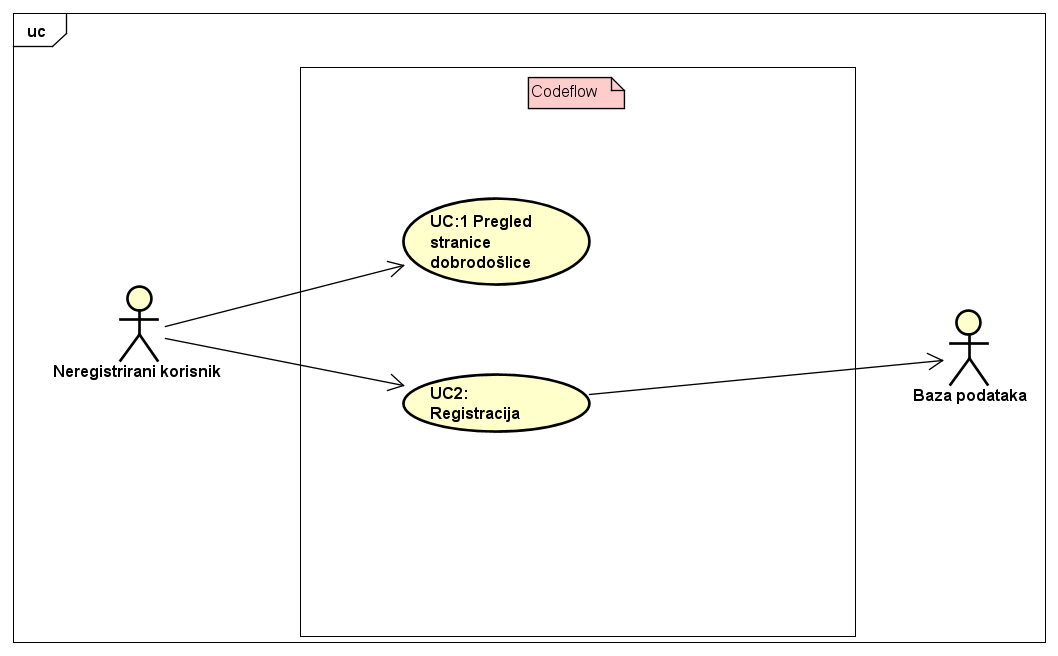
\includegraphics[width=\linewidth]{pictures/zahtjevi/nereg_korisnik.png}
				\caption{Zahtjevi neregistriranog korisnika}
				\label{fig:zahtjevi-nereg}
			\end{figure}
	
			\subsection{Zahtjevi registriranog korisnika}
			Nakon što se korisnik registrira postaju mu dostupne dodatne funkcionalnosti. Registriranom korisniku dostupna je mogućnost prijave s podacima koje je koristio za registraciju. Pošto se prijavi korisnik ima mogućnost pregledavanja ponuđenih zadataka i rang liste. Ponuđene zadatke može filtrirati na neki od dostupnih načina i dostupan mu je detaljniji pregled jednog od filtriranih zadataka. Prema podržanim funkcionalnostima modernih društvenih mreža, korisniku je predstavljena opcija filtriranja zadataka prema sljedećim kriterijima: 
			\begin{itemize}
				\item preporučeni zadaci
				\item zadaci slijeđenih korisnika
				\item najnoviji zadaci
			\end{itemize}
			Tijekom detaljnijeg pregleda odabranog zadatka prijavljenom su korisniku ponuđene opcije ocjenjivanja i komentiranja zadatka. Uz sam detaljniji opis zadatka, korisniku je moguć odabir nekog od rješenja gledanog zadatka. Odabrano rješenje registrirani korisnik može komentirati, a mogućnost ocjenjivanja zadatka omogućena mu je samo nakon rješavanja zadatka. Budući da je rješavanje zadatka preduvjet jednom od ostalih zahtjeva, ta je funkcionalnost također omogućena korisniku. Korisničko rješenje evaluirano je pomoću vanjskog izvršitelja programskog koda te nakon evaluacije spremljeno. Uz stvaranje rješenja programskih zadataka, prijavljenom korisniku ponuđena je opcija stvaranja programskog zadatka. Zahtjevi navedeni uz pregledavanja zadataka, rješavanje zadataka i stvaranje zadataka jezgreni su zahtjevi aplikacije.\\ Prijavljenom korisniku dostupna je mogućnost potpunog upravljanja vlastitim zadacima, rješenjima, komentarima i ocjenama. Pod tim se podrazumijevaju njihovo uređivanje i brisanje. Uz navedenu mogućnost upravljanja vlastitim zadacima, rješenjima, komentarima i ocjenama, prijavljenom korisniku omogućeno je mijenjanje vlastitih podataka. Po uzoru na određene mogućnosti društvenih mreža, prijavljenom korisniku su dostupne opcije pregleda profila drugih registriranih korisnika. Isto tako, korisnik može druge korisnike pratiti ili otpratiti. Osim mogućnosti pregleda tuđih korisničkih stranica, prijavljeni korisnik može vidjeti svoju korisničku stranicu. Detaljniji grafički prikazi ovih korisničkih zahtjeva vidljivi su na slikama \ref{fig:zahtjevi-korisnik1} i \ref{fig:zahtjevi-korisnik2}.
			\begin{figure}[H]
				\centering
				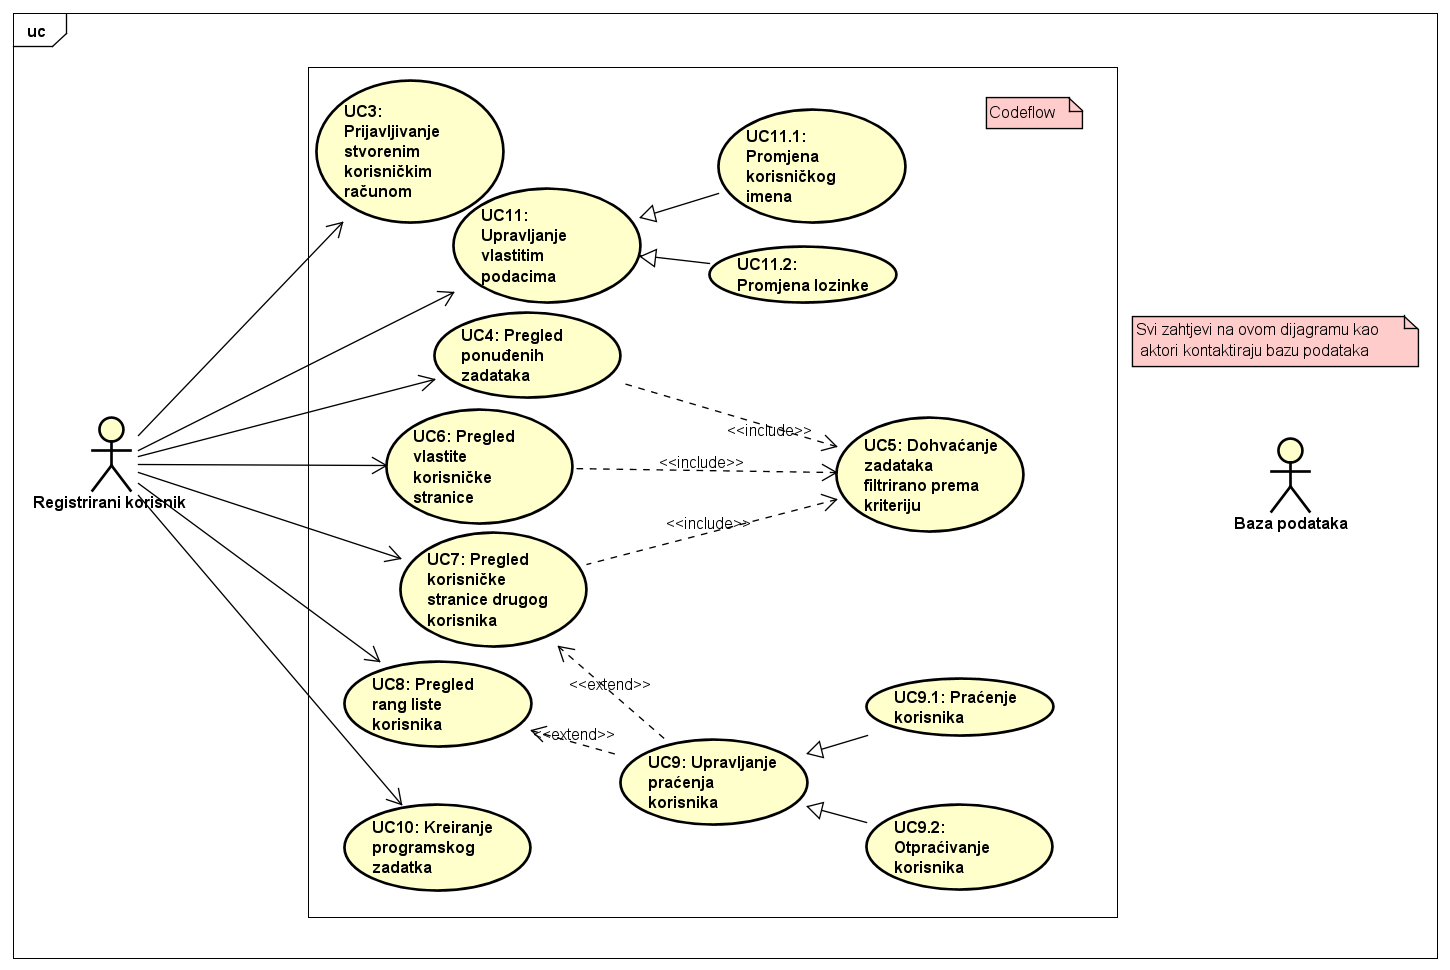
\includegraphics[width=\linewidth]{pictures/zahtjevi/korisnik1.png}
				\caption{Zahtjevi registriranog korisnika, prvi dio.}
				\label{fig:zahtjevi-korisnik1}
			\end{figure}
			\begin{figure}[H]
				\centering
				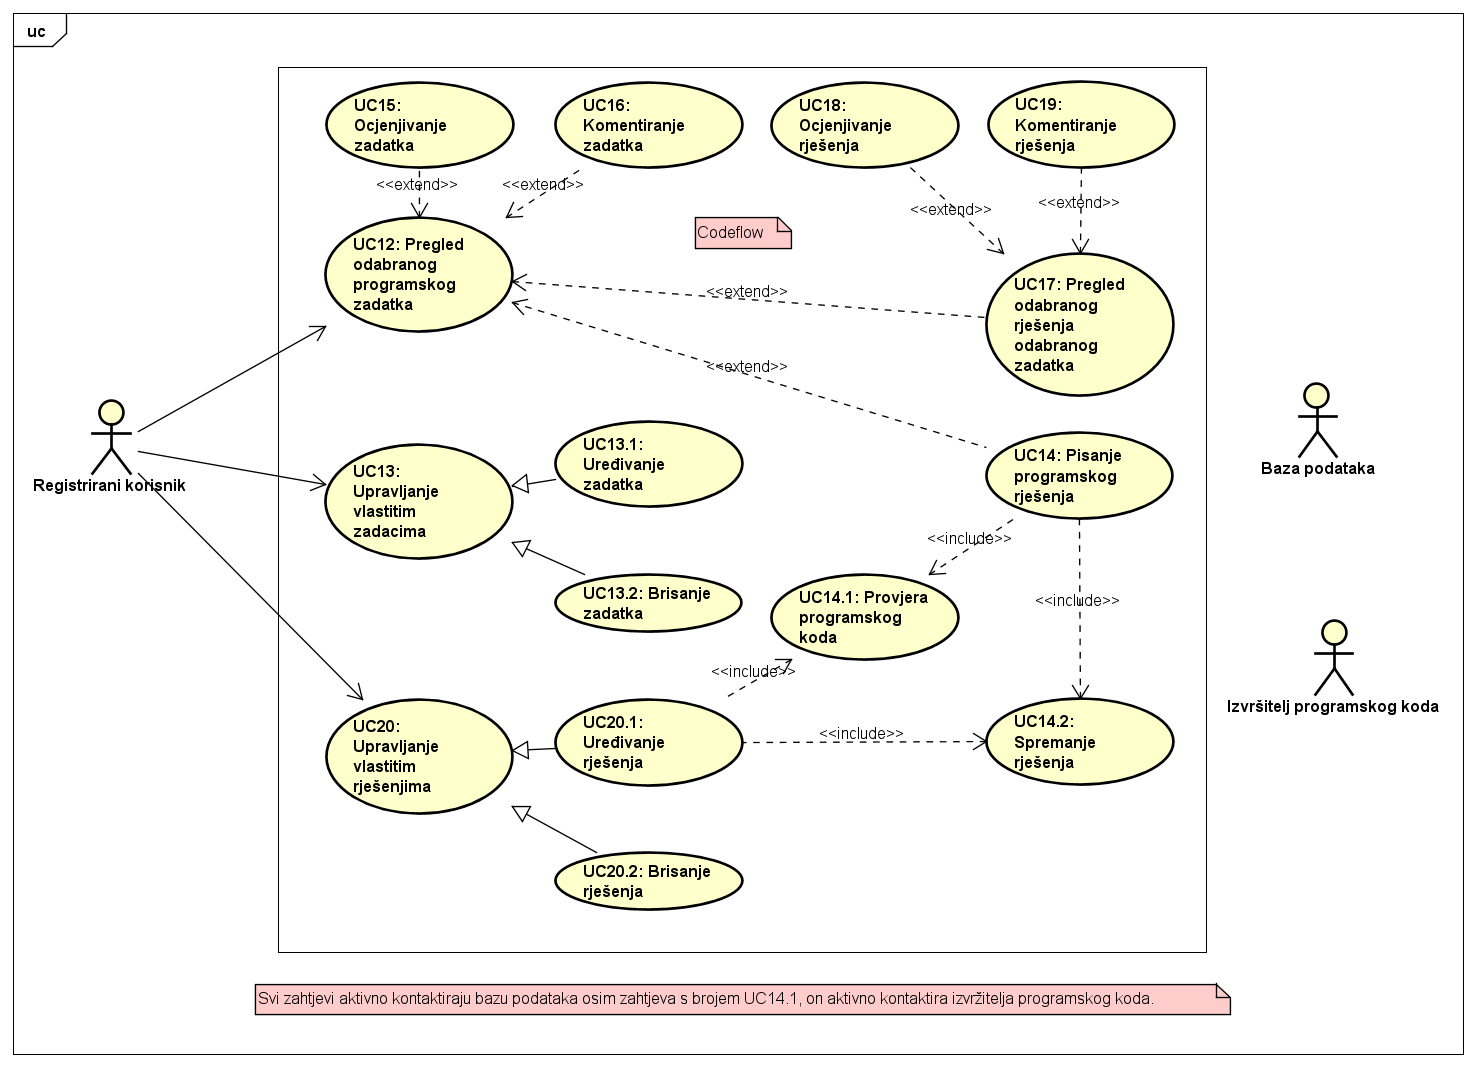
\includegraphics[width=\linewidth]{pictures/zahtjevi/korisnik2.png}
				\caption{Zahtjevi registriranog korisnika, drugi dio.}
				\label{fig:zahtjevi-korisnik2}
			\end{figure}
	
		\section{Nefunkcionalni zahtjevi}
		Nefunkcionalni zahtjevi, za razliku od funkcionalnih, ne opisuju koje mogućnosti sustav treba pružati nego koje karakteristike on treba imati. U slučaju promatrane internetske stranice, nefunkcionalni zahtjevi navedeni su unutar sljedeće liste:
		\begin{itemize}
			\item korisničke lozinke trebaju biti pravilno spremljene
			\item veza s bazom podataka i izvršiteljem programskog koda treba biti stabilna
			\item korisničko sučelje treba biti intuitivno za korištenje
			\item ostvarivanje evaluacije korisničkih rješenja treba biti unutar dvominutnog intervala 
		\end{itemize}
	
	\chapter{Postojeća programska rješenja i funkcionalnosti društvenih mreža}
	Poznata programska rješenja koja podržavaju funkcionalnost rješavanja programskih zadataka su:
	\begin{itemize}
		\item Leetcode\cite{Leetcode2021}
		\item Edgar\cite{Edgar2021}
		\item Codewars\cite{Codewars2021}
		\item HackerRank\cite{HackerRank2021}
	\end{itemize}
	
		\section{Leetcode}
		Leetcode je vjerojatno najveća i najpoznatija internetska aplikacija koja omogućava rješavanje programskih zadataka. Osnovana 2015. godine u Silicijskoj dolini, od samog početka bilježila je značajan rast i već 2017. godine imala preko milijun registriranih korisnika.\\
		Svrha i namjera Leetcode aplikacije jest priprema korisnika aplikacije na razgovore za posao pomoću specifično dizajniranih programskih zadataka. Pripremljeni zadaci slične su prirode kao i oni koje najpoznatije tehnološke firme predstavljaju svojim pristupnicima na razgovorima za posao. Preduvjet pristupu ponuđenim zadacima je registracija, a registrirani korisnici uz mogućnost rješavanja zadataka (koje mogu filtrirati po kriterijima) također mogu provoditi rasprave unutar foruma. Rasprave su često povezane s temom pitanja koje velike tehnološke tvrtke postavljaju. Bitno je napomenuti da Leetcode podržava programska rješenja pisana unutar četrnaest različitih programskih jezika. Rješenja zadataka mogu biti predložena unutar rasprave te dodatno komentirana od drugih korisnika.\\
		Ipak, postoje i neke funkcionalnosti koje nisu podržane unutar Leetcodea. Leetcode ne dopušta svojim registriranim korisnicima da sami dizajniraju svoje zadatke ili da prate korisnike koji su im se dojmili unutar diskusijskog foruma.\\
		Ukratko, Leetcode internetska aplikacija je veoma impresivna po broju funkcionalnosti koje nudi svojim registriranim korisnicima. Navedene funkcionalnosti napisane unutar ove sekcije najosnovnije su mogućnosti koje Leetcode nudi.
		\begin{figure}[H]
			\centering
			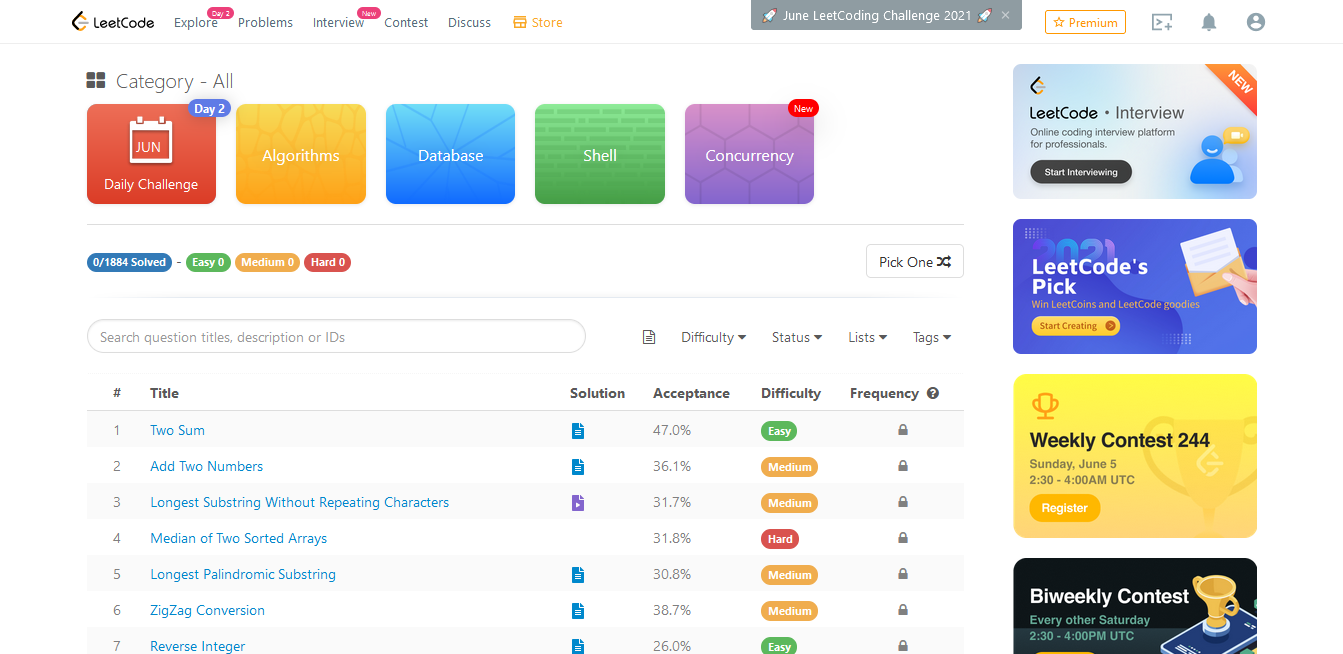
\includegraphics[width=\linewidth]{pictures/prikazi/Leetcode.png}
			\caption{Prikaz stranice Leetcode}
			\label{fig:leetcode}
		\end{figure}
	
		\section{Edgar}
		Edgar je internetska aplikacija koju Fakultet elektrotehnike i računarstva koristi u edukacijske svrhe, primarno kao sustav provođenja provjera vezanih uz temu programiranja. Na Fakultetu elektrotehnike i računarstva se intenzivno koristi zbog svojih mogućnosti definiranja i provođenja testova. \\
		Pristup internetskoj aplikacije moguć je samo ovlaštenim osobama pomoću njihovih korisničkih računa. Korisnici koji imaju ulogu predavača mogu definirati testove koje onda ostali studenti rješavaju nakon što se prijave sa svojim korisničkim računima. Edgar podržava mnoge programske jezike te tijekom rješavanja testnih zadataka vraća povratne informacije korisniku. Također, Edgar podržava stvaranja edukacijskih materijala poput edukacijskih vježbi. Isto tako, korisniku je na raspolaganju i pisanje proizvoljnog koda unutar "Code sandbox" funkcionalnosti stranice. Korisnici Edgara ne mogu ući u interakciju jedni s drugima.\\
		Internetska stranica Edgar primarno pruža funkcionalnosti provjere programskog koda. Ne fokusira se na interakciju korisnika te sadržava poveći broj funkcionalnosti od kojih su ovdje navedene samo osnovne.
		\begin{figure}[H]
			\centering
			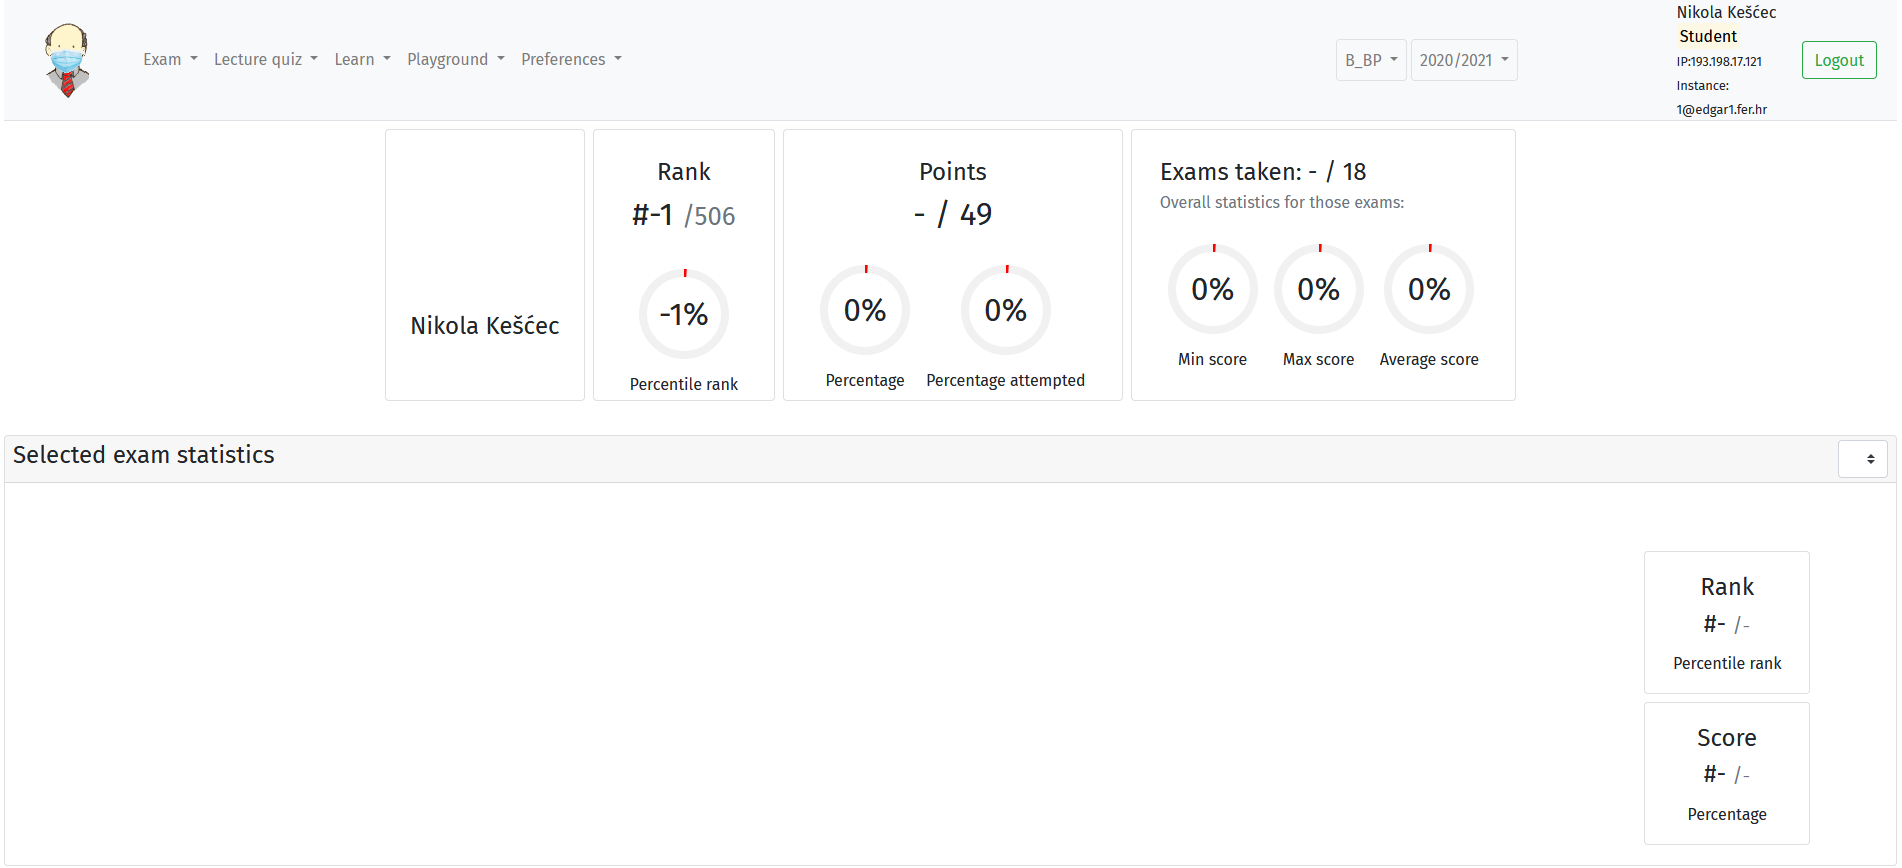
\includegraphics[width=\linewidth]{pictures/prikazi/Edgar.png}
			\caption{Prikaz stranice Edgar}
			\label{fig:edgar}
		\end{figure}
	
		\section{Codewars}
		\label{sec:codewars}
		Codewars internetska stranica po funkcionalnosti slična je Leetcodeu, ali uvodi dodatne mogućnosti rangiranja korisnika prema težini zadataka  (unutar stranice zvani \textit{kata}) koje rješavaju. Osnovana je 2012. godine, a  njezina namjera usavršavanje je znanja programskih jezika i proširenje znanja drugih jezika.\\
		\textit{Kate} su zadaci koji nose određenu količinu bodova, a definiraju ih korisnici Codewarsa. Svaka kata nosi određen broj bodova, zvani \textit{kyu}. Teži zadaci nose više bodova, a rješenja zadataka moguće je komentirati s ostalim korisnicima. Također, isto kao i sve već spomenute internetske stranice, Codewars pruža mogućnost rješavanja zadataka u različitim jezicima. Bitno je napomenuti da Codewars implementira sve popularniji proces "igrifikacije" \engl{gamification}. Taj proces uvodi razine i određene nagrade koje korisnike motiviraju za daljnje rješavanje sve težih zadataka.\\
		Tijekom registracije, korisnici trebaju proći inicijalizacijski test koji testira njihova osnovna znanja jednog od ponuđenih jezika i to je minimalno predznanje glavan je preduvjet budućeg korištenja stranice.
		\begin{figure}[H]
			\centering
			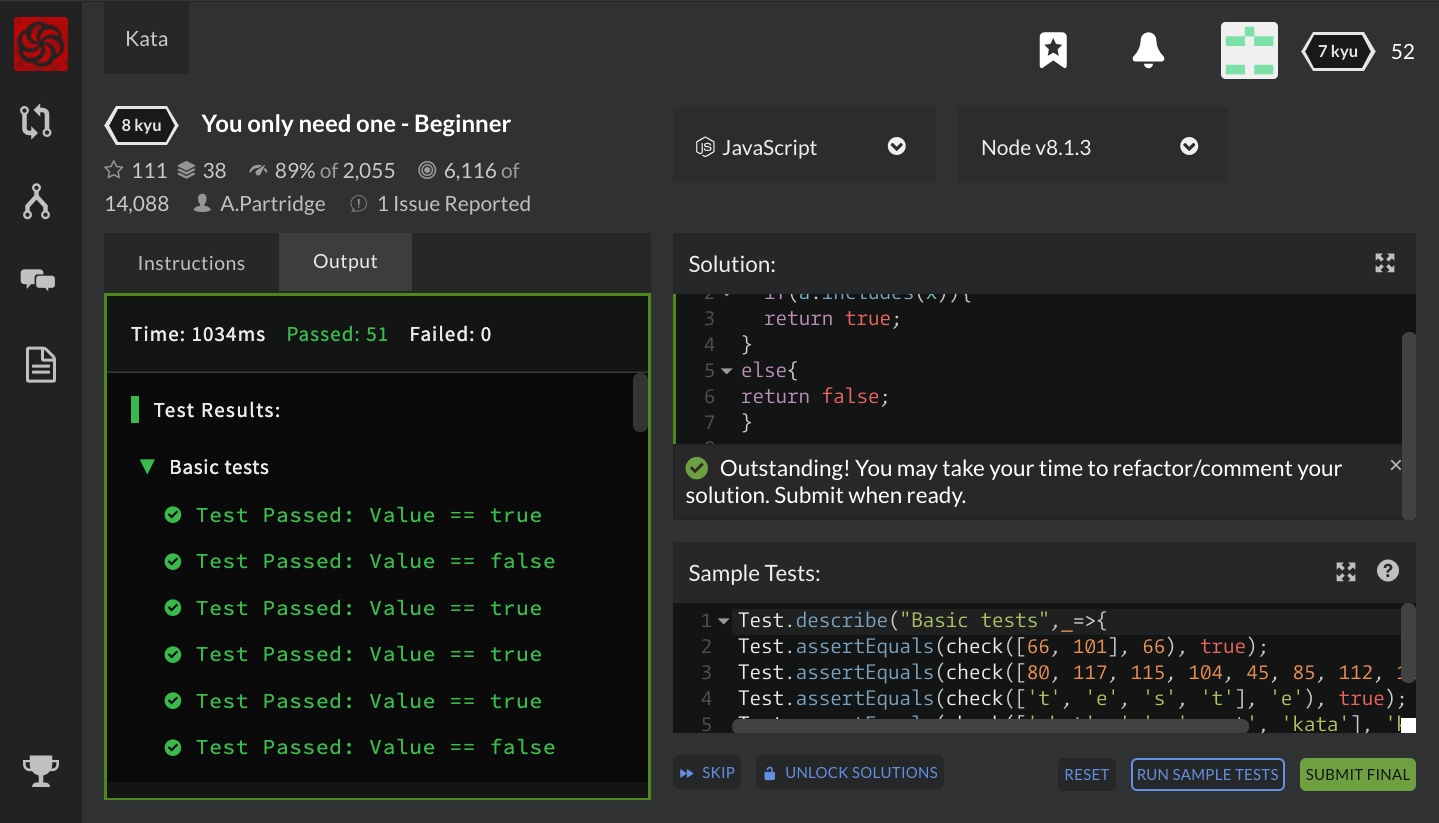
\includegraphics[width=\linewidth]{pictures/prikazi/Codewars.png}
			\caption{Prikaz rješavanja jedne \textit{kate}}
			\label{fig:codewars}
		\end{figure}
	
		\section{HackerRank}
		Internetska stranica HackerRank pruža drugačije usluge od već navedenih stranica. Namjera stranice je povezivanje programera s tvrtkama koje bi bile zainteresirane za njih, ali i učenje novih jezika, programskih algoritama te paradigmi.\\
		Stranica pruža mogućnost stvaranja računa korisnicima, ali i tvrtkama koje interesira HackerRank. Mogućnost rješavanja programskih zadataka omogućena je za korisnike i tvrtke, a nerijetko stranica organizira i natjecanja zvana "CodeSprints". Na tim natjecanjima korisnici rješavaju iste programske zadatke. HackerRank stranica predana rješenja rangira prema njihovoj točnosti i kvaliteti. Autore tih rješenja također rangira na HackerRank ljestvici korisnika, te, kao i Codewars, provodi proces "igrifikacije".\\
		Mogućnosti HackerRank stranice raspodijeljene su između različitog tipa korisnika: regularnog korisnika i tvrtke. Korisnicima pruža mogućnosti rješavanja zadataka u svrhu promocije te onim korisnicima koji traže posao potencijalno može pomoći u tomu.
		\begin{figure}[H]
			\centering
			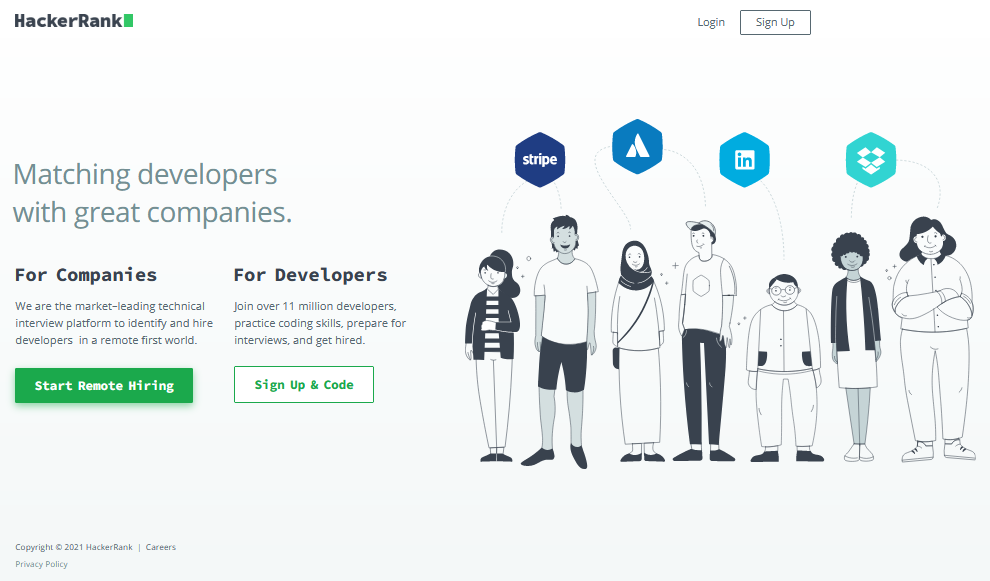
\includegraphics[width=\linewidth]{pictures/prikazi/HackerRank.png}
			\caption{Prikaz stranice dobrodošlice HackerRank internetske stranice}
			\label{fig:hackerrank}
		\end{figure}
	
		\section{Zajedničke funkcionalnosti i dodatak funkcionalnosti društvenih mreža}
		Vidljivo je iz bližeg razmatranja navedenih stranica da svaka od stranica ima različitu namjeru te u različite svrhe koristi funkcionalnost zadavanja i rješavanja zadataka. Stranice Codewars, Leetcode i HackerRank donekle su slične po funkcionalnostima koje pružaju, ali ipak razlikuju se podosta u namjeri. Edgar je različit od navedenih stranica jer njegova je svrha prvenstveno akademske i edukacijske prirode. Ipak, navedene stranice imaju nekoliko dijeljenih funkcionalnosti:
		\begin{itemize}
			\item stvaranje zadataka (Edgar i Codewars)
			\item rješavanje zadataka
			\item provjera rješenja zadataka
			\item komentiranje rješenja (Codewars, Leetcode, HackerRank)
		\end{itemize}
		Bitno je također uvidjeti da dio stranica pruža određene mogućnosti društvenih mreža, kao što su već spomenuto komentiranje rješenja te mogućnost određene interakcije s korisnicima. Ipak, mogućnosti praćenja korisnika kod velikog dijela stranica nisu moguće, a isto tako direktno ocjenjivanje rješenja nije podržano na svim stranicama. Nerijetko su i određene funkcionalnosti stranica moguće samo korisnicima koji plaćaju određenu pretplatu (poput pregleda službenog rješenja nekog programskog zadatka).
		Ono što Codeflow stranica sadržava unutar sebe jest spoj navedenih najčešćih funkcionalnosti promotrenih stranica i jezgrenih funkcionalnosti modernih društvenih mreža. Te jezgrene funkcionalnosti su:
		\begin{itemize}
			\item praćenje korisnika
			\item komentiranje na objavljene sadržaje drugih korisnika (uključujući vlastite)
			\item ocjenjivanje sadržaja drugih korisnika
			\item pregledavanje profila drugih korisnika
		\end{itemize}
	
	
	\chapter{Korištene tehnologije}
	\label{cha:tehnologije}
	Arhitektura modernih internetskih aplikacija najčešće se sastoji od tri sloja:
	\begin{itemize}
		\item korisničkog ili prezentacijskog sloja
		\item poslovnog sloja
		\item podatkovnog sloja
	\end{itemize}
	Tijekom razvoja internetske aplikacije Codeflow korištene su tehnologije koje se uglavnom mogu smjestiti unutar jednog od ta tri sloja te su one po slojevima dodatno pojedinačno razmotrene.
	
		\section{Tehnologije prezentacijskog sloja}
		Korištene tehnologije prezentacijskog sloja pisane su JavaScript\cite{JavaScript2021} programskim jezikom jer on je jedini programski jezik kojeg internetski preglednici podržavaju. Ipak, razvoj JavaScript aplikacija ne događa se isključivo unutar internetskih preglednika, a podršku za razvoj i izvođenje izvan spomenutih preglednika omogućava Node.js\cite{Nodejs2021} platforma. Node.js platforma je cjelokupno pokretačko okruženje koje pomoću komponente \textit{V8 JavaScript engine}\cite{V82021}  izvodi JavaScript programski kod izvan internetskog preglednika. Node.js također unutar sebe sadržava upravitelja paketima, NPM\cite{NPM2021} (Node Package Manager), koji pruža mogućnost korištenja velikog broja različitih dodataka i biblioteka  \engl{libraries} pisanih jezikom JavaScript.
		
		\subsubsection{Single Page Application tip stranica}
		SPA\cite{SPA2021} \engl{Single page Application} tip internetskih aplikacija pri promjeni stranice ne dohvaćaju HTML datoteku sa sadržajem nove stranice već dinamički prepisuju sadržaj trenutačne stranice uz pomoć JavaScript programskog jezika te podataka dobivenih s internetskog poslužitelja. Cilj \textit{Single Page Application} tipa internetske aplikacije jest doživljaj korištenja aplikacije učiniti sličnim onomu kojeg imaju aplikacije pokrenute na računalu.\\ 
		Budući da se stranice mijenjaju isključivo manipulacijom elemenata DOM-a \engl{Document Object Model}, tijekom korištenja aplikacije učitavanje stranice potrebno je obaviti samo jednom tijekom prvog pristupa stranici. Glavni nedostaci SPA internetskih aplikacija jesu sporo prvo učitavanje internetske aplikacije i loša optimizacija zastupljenosti tijekom pretrage internetskim pretraživačima. Sporo učitavanje aplikacije uzrokovano je potrebom za učitavanjem cjelokupne internetske aplikacije tijekom prvog pristupa stranici, a loša optimizacija zastupljenosti tijekom pretrage inicijalnim nedostatkom HTML-a prilikom inicijalnog učitavanja. Ipak, brzina odaziva na korisničke zahtjeve uveliko unaprjeđuje korisničko iskustvo, pa je upravo korisničko sučelje Codeflow aplikacije SPA tip internetske aplikacije. Kratak pregled interakcije i arhitekture SPA tipa internetske aplikacije i internetskog poslužitelja prikazan je na slici \ref{fig:spa}.
		\begin{figure}[H]
			\centering
			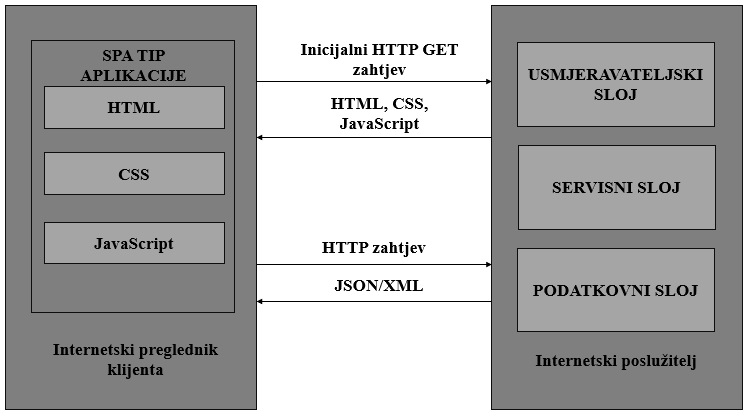
\includegraphics[width=\linewidth]{pictures/prikazi/SPA.png}
			\caption{Prikaz općenite interakcija i arhitekture SPA tipa internetskih aplikacija}
			\label{fig:spa}
		\end{figure}
				
			\subsection{React i React Router}
			React\cite{react2021} je biblioteka kojoj je svrha izrada korisničkih sučelja \engl{user interface}. Otvorenog je koda te ga razvijaju i održavaju različite tvrtke (od kojih je najbitnija Facebook jer ona ga je zapravo i začela) i različiti individualni programeri. Prva verzija Reacta na tržište je izašla 2013. godine, a od tada njegova popularnost kontinuirano raste. Reactov fokus jest razvoj dinamičnih i lagano nadogradivih korisničkih sučelja. React laganu nadogradivost ostvaruje putem komponentno usmjerenog razvoja, što znači da svaka razvijana funkcionalnost enkapsulira unutar sebe svu logiku i izgled koji su potrebni za njezin rad. Sve komponente mogu unutar sebe sadržavati druge komponente, tako ostvarujući kompoziciju \engl{composition} komponenata, a njenim korištenjem razvijanje složenih korisničkih sučelja postaje jasno i strukturirano. React biblioteka spomenute komponente koristi za izgradnju konkretnog dokumenta objektnog modela koji kasnije biva prikazivan korisniku. Kako korisnička interakcija ne bi bila spora, React interno održava posebnu strukturu podataka, virtualni dokument objekt model, koja pamti stanje komponenata. Ako se ikoja komponenta promijeni, React samo promijenjenu komponentu ažurira unutar stvarnog modela objekta dokumenta. Tim pristupom održava responzivnost korisničkog sučelja.\\
			\begin{figure}[H]
				\centering
				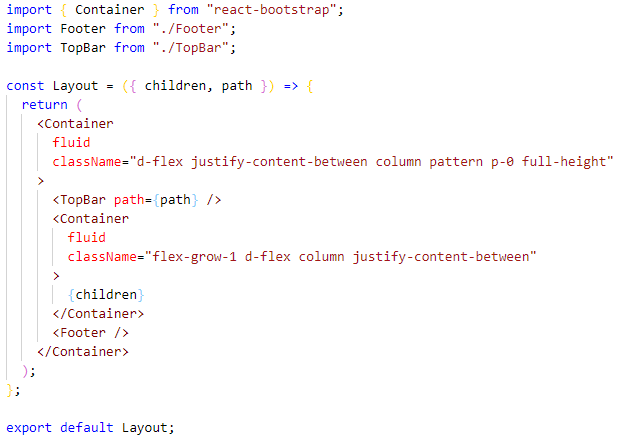
\includegraphics[scale=0.75]{pictures/prikazi/React.png}
				\caption{Primjer jednostavnije kompozicije komponenata unutar Reacta}
				\label{fig:react}
			\end{figure}
			React Router\cite{react-router2021} dodatak je React biblioteci koja služi za usmjeravanje između različitih dostupnih  stranica razvijenih pomoću React komponenata. Pomoću njegovih funkcionalnosti ostvaruju se značajke SPA tipa aplikacije jer React Router preusmjeravanje stranica obavlja isključivo unutar internetskog preglednika klijenta. Deklariranjem specifičnih URL-a \engl{Uniform Resource Locator} te korištenjem specijalnih \textit{Link} React komponenata klijentu je omogućeno mijenjanje stranica.
			\begin{figure}[H]
				\centering
				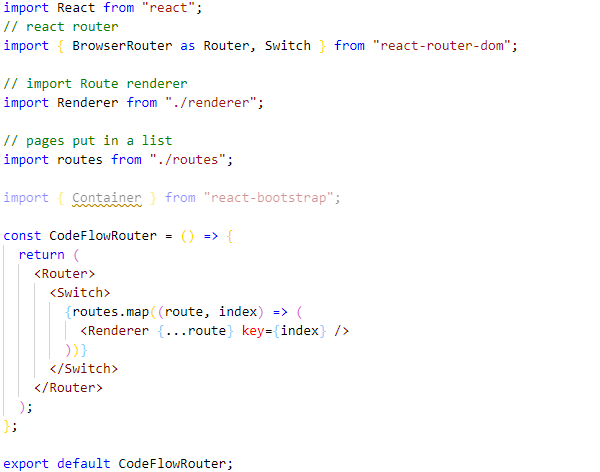
\includegraphics[scale=0.75]{pictures/prikazi/ReactRouter.png}
				\caption{Primjer korištenja React Routera.}
				\label{fig:react-router}
			\end{figure}
			
			\subsection{Bootstrap}
			Bootstrap\cite{bootstrap2021} je radni okvir \engl{framework} otvorenog koda namijenjen dizajnu i prilagođavanju responzivnih internetskih stranica s mnoštvom definiranih komponenata, izgleda i predložaka. Temeljen je na CSS stilskom jeziku te, uz pomoć JavaScript programskog jezika osigurava jednakost izgleda neovisno o platformi. Održava ga tvrtka Twitter te mnogi individualni programeri. Bootstrap, osim što omogućava dizajn stranice, podržava i lagano raspoređivanje elemenata stranice korištenjem ugrađenih svojstava CSS-a. Boostrap se koristi pomoću ugrađenih klasa, a postoje i određeni prilagodni radni okviri koji Bootstrap omogućavaju u drugim radnim okvirima ili bibliotekama (dobar primjer je React Bootstrap za React).
			\begin{figure}[H]
				\centering
				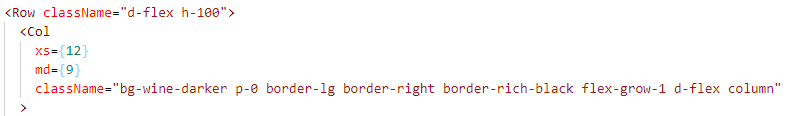
\includegraphics[width=\linewidth]{pictures/prikazi/Bootstrap.png}
				\caption{Primjer korištenja React-Bootstrapa i Bootstrap klasa unutar Reacta.}
				\label{fig:bootstrap}
			\end{figure}
			
			\subsection{Material-UI}
			Material-UI\cite{materialUI2021} je radni okvir otvorenog koda koji omogućava korištenje gotovih dijelova korisničkog sučelja koja prate načela \textit{material designa}. Specijaliziran je za React biblioteku te se bilo koja Material-UI komponenta može koristiti kao obična React komponenta. Podržava i potpunu prilagodbu raspoloživih komponenata.
			\begin{figure}[H]
				\centering
				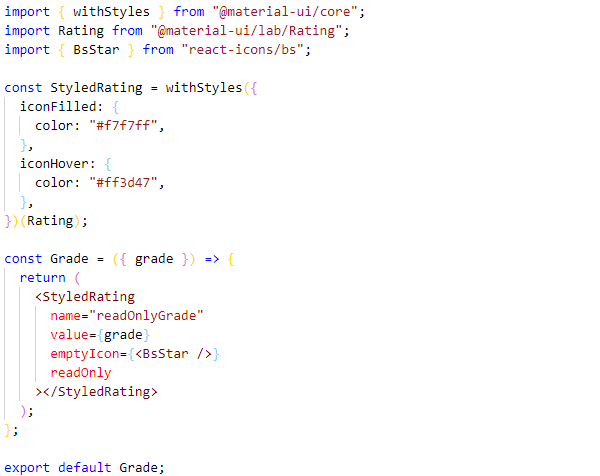
\includegraphics[scale=0.75]{pictures/prikazi/MaterialUI.png}
				\caption{Primjer korištenja Material-UI komponenata unutar Reacta.}
				\label{fig:materialUI}
			\end{figure}
			
			\subsection{Ace}
			Ace\cite{ace2021} je uređivač programskog koda namijenjen za lagano integriranje unutar internetske stranice ili JavaScript aplikacije. Otvorena je koda te podržava sve funkcionalnosti koje uobičajen uređivač teksta podržava. Budući da je prvotno namijenjen pisanju programskog koda, podržava mnoštvo različitih jezika. Ima mogućnosti naglašavanje sintakse odabranog podržanog programskog jezika, a također implementira rudimentarno nadopunjavanje programskog koda. Uz sve napomenute mogućnosti, sadržava različite teme te se one mogu mijenjati tijekom korištenja uređivača.
			\begin{figure}[H]
				\centering
				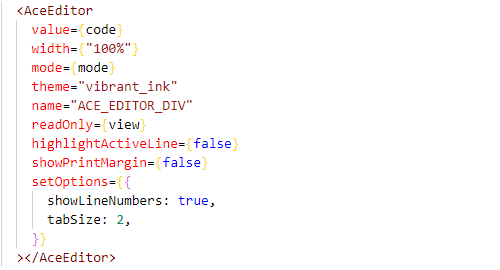
\includegraphics[scale=0.75]{pictures/prikazi/AceEditor.png}
				\caption{Primjer korištenja Ace-Editor React komponente.}
				\label{fig:ace}
			\end{figure}
	
		\section{Tehnologije poslovnog sloja}
		Korištene tehnologije poslovnog sloja temeljene su na programskom jeziku Javi\cite{java2021}. Uz Javu korišten je i Maven\cite{maven2021}, alat za upravljanje projektom koji nudi mogućnosti upravljanja Java ovisnostima \engl{dependencies}. Java ovisnosti su već napisani Java paketi koji proširuju osnovnu Javinu funkcionalnost.
			\subsection{Spring, Spring Boot i povezane tehnologije}
			Spring\cite{spring2021} je radni okvir za različite programske jezike, od kojih je jedan Java. Otvorena je koda te podliježe svim zahtjevima modernih radnih okvira, a namjera mu je da olakša razvoj modernih poslovnih aplikacija. Razvoj olakšava pružanjem implementacija često korištenih funkcionalnosti i pružanjem mogućnosti uključivanja novih. Temeljna tehnika kojom Spring omogućuje uključivanje novih funkcionalnosti jest inverzija upravljanja \engl{inversion of control} koja omogućava radnom okviru da transparentno poziva klijentski kod korištenjem različitih dobro poznatih oblikovnih obrazaca \engl{design patterns}. Inverziju upravljanja Spring radni okvir postiže korištenjem injekcije ovisnosti \engl{dependency injection}, a ona je zapravo mogućnost radnog okvira da zadovolji tražene objektne ovisnosti. Drugim riječima, radni okvir Spring sam stvara potrebne objekte te ih "injektira" tamo gdje su traženi (za razliku od tradicionalnog pristupa gdje korisnik sam stvara tražene objekte). Sama implementacija funkcionalnosti injekcije ovisnosti unutar Springa veoma je složena, ali uporaba funkcionalnosti izrazito je jednostavna. Tražene objekte potrebno je anotirati s posebnom anotacijom \textit{@Autowired}. Objekte koje treba stvoriti potrebno je anotirati s \textit{@Bean} anotacijom. Pomoću tih anotacija, Spring može sam stvoriti i injektirati objekt. Inverzija ovisnosti i injekcija ovisnosti omogućava Springu prilagodljiv i skalabilan razvoj, što ga čini veoma pogodnim za razvoj internetskih aplikacija. Dodatno, da bi održao kvalitetnu strukturu razvijane aplikacije, Spring preporuča internu raspodjelu Spring aplikacije u tri sloja: "\textbf{Controller}" sloj (definira interakciju s klijentskim zahtjevima), "\textbf{Service}" sloj (ostvaruje temeljne funkcionalnosti) i "\textbf{Repository}" sloj (ostvaruje interakcije s podatkovnim slojem sveukupne aplikacije).\\
			Spring radni okvir podržava velik broj dodataka koji zadovoljavaju različite korisničke potrebe, a od njih su korištene Spring Security\cite{springsecurity2021} i Spring Data JPA\cite{springdatajpa2021}.
			\begin{figure}[H]
				\centering
				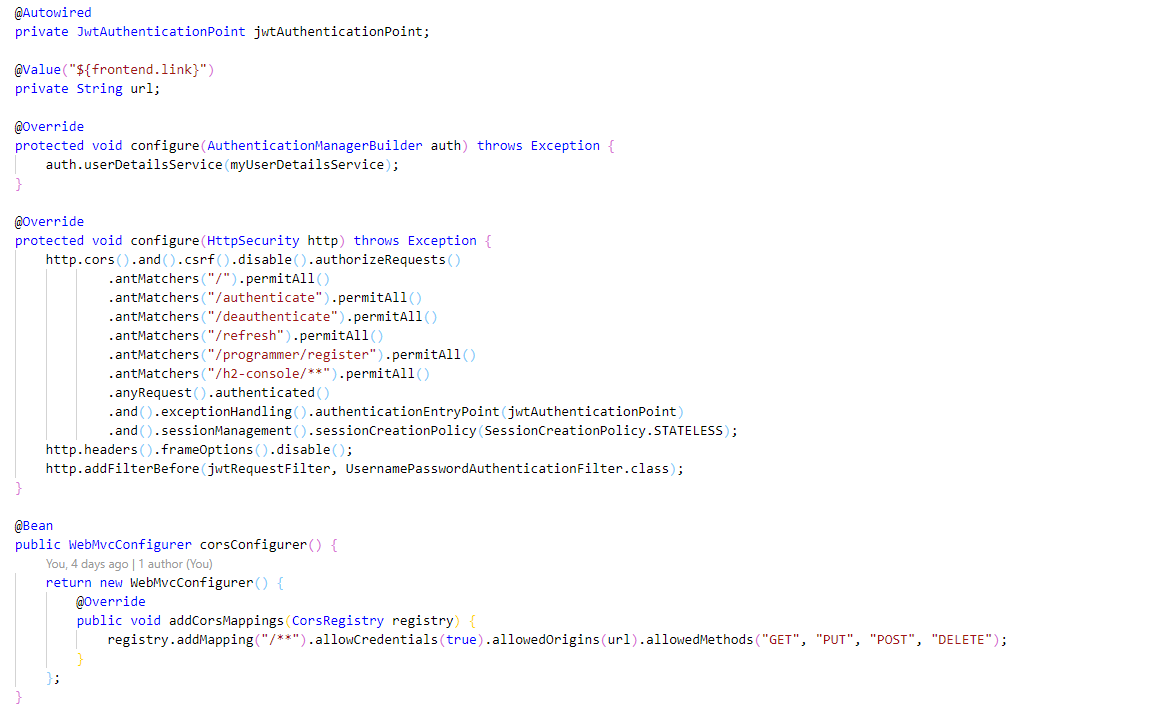
\includegraphics[width=\linewidth]{pictures/prikazi/Spring.png}
				\caption{Primjer injekcije ovisnosti te @Autowired i @Bean anotacija unutar Springa.}
				\label{fig:spring}
			\end{figure}
			
			\subsubsection{Spring Security}
			Spring Security je dodatak Spring radnom okviru koji transparentno omogućava autentifikaciju \engl{authentication} (proces je prikazan na slici \ref{fig:springsec}) i autorizaciju \engl{authorization} dijelovima razvijene aplikacije . Autentifikacija je proces provjere identiteta korisnika, a autorizacija je provjera prava korištenja resursa kojeg korisnik traži. Spring Security te funkcionalnosti ostvaruje korištenjem lanaca filtera \engl{filter chains} od kojih svaki provjerava određene dijelove korisničkog zahtjeva.
			\begin{figure}[H]
				\centering
				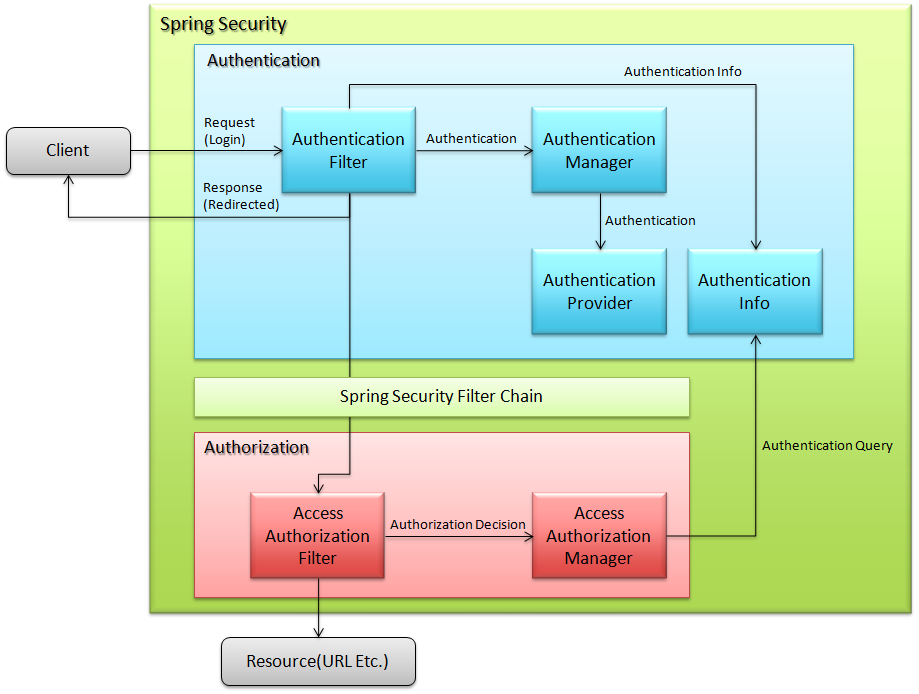
\includegraphics[width=\linewidth]{pictures/prikazi/SpringSecurity.png}
				\caption{Prikaz procesa autentifikacije unutar Spring Securityja.}
				\label{fig:springsec}
			\end{figure}
			
			\subsubsection{Spring Data JPA}
			\label{subsubsec:spingdatajpa}
			Spring Data JPA proširuje Spring radni okvir i njegov je cilj smanjenje količine programskog koda potrebnog za interakciju s podatkovnim slojem. Kao što mu i u imenu piše, Spring Data JPA podliježe JPA (skraćenica za Jakarta Persistence) specifikaciji. JPA nije ništa drugo doli specifikacija za upravljanje relacijskim podacima te upitnim jezikom \engl{query language} JPQL-om. Spring Data JPA za implementaciju specifikacije koristi Hibernate ORM (\ref{subsec:hibernate}).
			\subsubsection{Spring Boot}
			Naposlijetku, Spring Boot modul je Spring radnog okvira koji smanjuje broj konfiguracija Springa potrebnih za rad. Također uključuje početne ovisnosti, poput integriranog poslužitelja.
			\subsection{Hibernate}
			\label{subsec:hibernate}
			Hibernate\cite{hibernate2021} je radni okvir koji pruža automatsko preslikavanje razreda definiranih u programskog kodu u odgovarajuće relacije relacijske baze podataka. Takav tip radnih okvira znan je još kao ORM \engl{object-relational mapping} radni okviri. Implementiranje JPA specifikacije čini ga kompatibilnim sa Spring Data JPA proširenjem (\ref{subsubsec:spingdatajpa}), a njegova se funkcija može shvatiti kao most između baze podataka \engl{database} i podatkovnog sloja aplikacije. Funkcionalnost preslikavanja između različitih oblika podataka (programskih razreda i relacija) ostvaruje generiranjem i izvršavanjem SQL upita.
	
	
		\section{Tehnologije podatkovnog sloja}
		Unutar podatkovnog sloja koristi se relacijska baza podataka. Interakcija s njom odvija se korištenjem SQL-a \engl{Structured Query Language}.
			\subsection{PostgreSQL}
			PostgreSQL\cite{postgresql2021} je sustav za upravljanje bazom podataka otvorena koda. Dizajniran je za obradu i pohranu velike količine podataka. Popularan je i zbog toga ga podržavaju mnogi ORM radni okviri poput Hibernatea.
			\section{Pomoćne tehnologije}
			Tehnologije koje se same po sebi ne mogu svrstati ni u jedan od navedenih glavnih slojeva spomenute su u ovom potpoglavlju.
			\subsection{Axios}
			Axios\cite{axios2021} je lagan HTTP \engl{Hypertext Transfer Protocol} klijent pisan u JavaScriptu. Podržava asinkrono slanje zahtjeva, funkcionalnost presretanja i modificiranje zahtjeva i odgovora. 
			\begin{figure}[H]
				\centering
				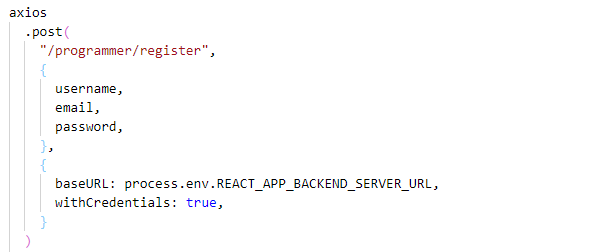
\includegraphics[scale=0.65]{pictures/prikazi/Axios.png}
				\caption{Primjer slanja POST zahtjeva pomoću Axiosa.}
				\label{fig:axios}
			\end{figure}
			\subsection{Judge0}
			Judge0\cite{judge02021} je izvršitelj programskoga koda otvorena koda kojeg Codeflow aplikacija koristi za provjeravanje rješenja pisanih za korisničke programske zadatke. Skalabilne je arhitekture te podržava preko 60 programskih jezika. Uz podršku prevođenja i izvođenja jednodatotečnih rješenja, Judge0 podržava prevođenje te izvođenje programskih rješenja koja se sastoje od više datoteka. Omogućava konfiguriranje postavki korištenih prevoditelja, postavljanje argumenata komandne linije te još mnogo drugih funkcionalnosti.
			\subsection{Git}
			Git\cite{git2021} je sustav za upravljanje izvornim kodom distribuiranog tipa otvorena koda \engl{distributed version control}. Upravljanje izvornim kodom vrši se pohranjivanjem koda unutar Git repozitorija koji mogu biti udaljeni ili lokalni. Udaljeni repozitoriji \engl{remote} najčešće su smješteni unutar nekog oblaka \engl{cloud} na nekoj Git platformi (primjer takve platforme je GitHub). Budući da je sustav distribuiran, lokalni repozitoriji sadržavaju svu povijest programskog koda koju i udaljeni. Inicijalne promjene izvornog koda događaju se unutar lokalnog repozitorija te tek nakon što se spreme unutar lokalnog repozitorija mogu se poslati na udaljeni repozitorij. Korištenje Gita osigurava strukturirano i kvalitetno praćenje te spremanje projekta.
	
	\chapter{Arhitektura rješenja}
		\section{Domena rješenja}
		\label{sec:domenarjesenja}
		Domena rješenja ostvarena je definicijom relacijske baze podataka pomoću PostgreSQL sustava za upravljanje bazama. Iako korišteni ORM Hibernate podržava \textit{code-first} pristup definiranja baze podataka (tablice se definiraju  programskim razredima, a ne programski razredi tablicama) ipak je odabran pristup gdje se prvo definira shema korištene baze podataka \engl{database-first}. Iz tog je razloga shema baze podataka koja opisuje domenu problema Codeflow aplikacije sa svim tablicama i njihovim međusobnim vezama prikazana na slici \ref{fig:db}.
		\begin{figure}[H]
			\centering
			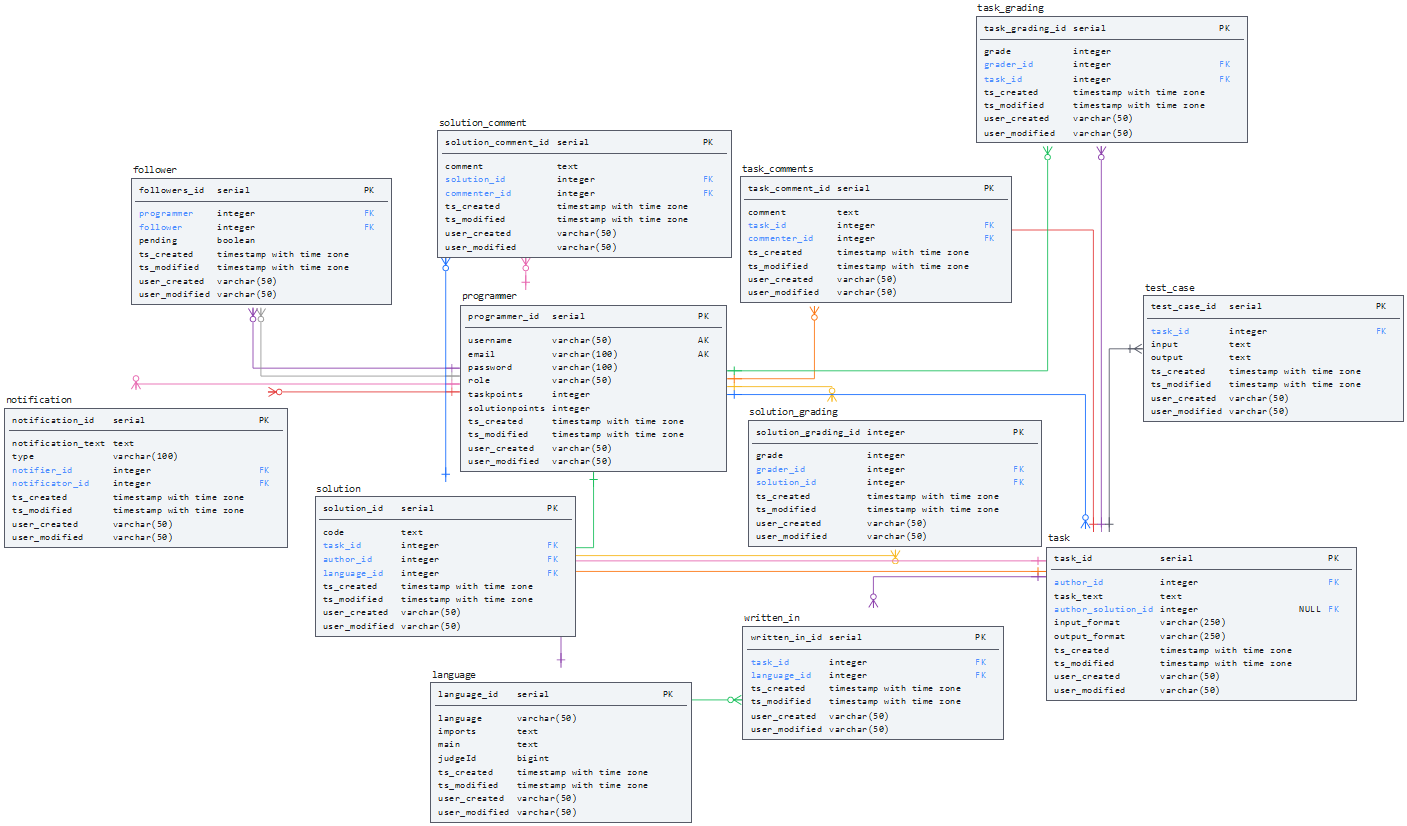
\includegraphics[width=\linewidth]{pictures/prikazi/Database.png}
			\caption{Kompletan prikaz sheme Codeflow baze podataka.}
			\label{fig:db}
		\end{figure}
		Valja napomenuti da sve tablice dijele atribute ts\_created, ts\_modified, user\_created, user\_modified radi lakšeg praćenja stvaranja i promjena točnih zapisa unutar tablica, a jer su dijeljeni neće biti dodatno spomenuti tijekom detaljnijeg opisa svake tablice. Same tablice oblikovane su prema korisničkim zahtjevima (definirani u poglavlju \ref{cha:zahtjevi}).
		\begin{table}[H]
			\caption{Dijeljeni atributi}
			\label{tbl:dij-attr}
			\centering
			\begin{tabu} to \textwidth {XXX}
				\tabucline[1.75pt]{-}
				\textbf{Ime atributa} & \textbf{Tip} & \textbf{Opis}\\				
				\tabucline[1.75pt]{-}
				ts\_created & timestamp with timezone & vrijeme nastanka\\ \hline
				ts\_modified & timestamp with timezone & vrijeme modifikacije\\ \hline
				user\_created & varchar(50) & korisnik koji je napravio zapis\\ \hline
				user\_created & varchar(50) & korisnik koji je zadnji modificirao zapis\\
				\tabucline[1.75pt]{-}
			\end{tabu}
		\end{table}
		
		Tablica \textbf{programer} opisuje korisnika aplikacije Codeflow te predstavlja centralnu tablicu. Stvara se tijekom registracije korisnika te pohranjuje sve korisničke informacije. Vlastiti atributi tablice programer su programmer\_id, username, email, password, role, taskpoints i solutionpoints. Role atribut je dodan, ali unutar ove verzije različite korisničke uloge nisu implementirane.
		\begin{table}[H]
			\caption{Tablica programmer}
			\label{tbl:programmer}
			\centering
			\begin{tabu} to \textwidth {XXX}
				\tabucline[1.75pt]{-}
				\textbf{Ime atributa} & \textbf{Tip} & \textbf{Opis}\\ 				
				\tabucline[1.75pt]{-}
				\textbf{programmer\_id} & integer & surogatni primarni ključ\\ \hline
				username & varchar(50) & korisnikovo korisničko ime, mora biti jedinstveno\\ \hline
				email & varchar(100) & korisnikov e-mail, mora biti jedinstven\\ \hline
				password & varchar(100) & \textit{hash} korisnikove lozinke\\ \hline
				role & varchar(50) & korisnikova uloga\\ \hline
				taskpoints & integer & bodovi koje je korisnik dobio zbog kvalitete svojih zadataka\\ \hline
				solutionpoints & integer &  bodovi koje je korisnik dobio zbog kvalitete svojih rješenja\\
				\tabucline[1.75pt]{-}
			\end{tabu}
		\end{table}
		
		Tablica \textbf{task} opisuje zadatak kojeg je korisnik napravio. Tijekom stvaranja zadatka spremaju se novi podaci unutar tablice task, ali i unutar tablice test\_case jer ti podaci su neophodni za dinamičku provjeru ispravnosti zadatka. Vlastiti atributi tablice task su task\_id, author\_id, task\_text, author\_solution\_id, input\_format i output\_format.
		\begin{table}[H]
			\caption{Tablica task}
			\label{tbl:task}
			\centering
			\begin{tabu} to \textwidth {XXX}
				\tabucline[1.75pt]{-}
				\textbf{Ime atributa} & \textbf{Tip} & \textbf{Opis}\\ 				
				\tabucline[1.75pt]{-}
				\textbf{task\_id} & integer & surogatni primarni ključ\\ \hline
				author\_id & integer & strani ključ autora zadatka\\ \hline
				task\_text & text & tekst zadatka\\ \hline
				author\_solution\_id & integer & autorovo rješenje (nije nužno)\\ \hline
				input\_format & varchar(250) & primjer ulaza\\ \hline
				output\_format & varchar(250) & primjer izlaza\\ \hline
				\tabucline[1.75pt]{-}
			\end{tabu}
		\end{table}
	

		Tablica \textbf{solution} opisuje rješenje kojeg je korisnik napravio. Vlastiti atributi tablice solution su solution\_id, code, task\_id, author\_id, task\_text i language\_id.
		\begin{table}[H]
			\caption{Tablica solution}
			\label{tbl:solution}
			\centering
			\begin{tabu} to \textwidth {XXX}
				\tabucline[1.75pt]{-}
				\textbf{Ime atributa} & \textbf{Tip} & \textbf{Opis}\\ 				
				\tabucline[1.75pt]{-}
				\textbf{solution\_id} & integer & surogatni primarni ključ\\ \hline
				code & text & kod rješenja\\ \hline
				task\_id & integer & strani ključ zadatka rješenja\\ \hline
				author\_id & integer & strani ključ autora zadatka\\ \hline
				language\_id & integer & strani ključ jezika u kojem je rješenje pisano\\ \hline
				\tabucline[1.75pt]{-}
			\end{tabu}
		\end{table}
	
		Tablica \textbf{notification} opisuje obavijest koja biva poslana korisniku tijekom nekog događaja unutar aplikacije. Vlastiti atributi tablice notification su notification\_id, notification\_text, type, notifier\_id, notificator\_id. Prate se tipovi obavijesti jer ovisno o njima vizualno se razlikuju prikazane notifikacije.
		\begin{table}[H]
			\caption{Tablica notification}
			\label{tbl:notification}
			\centering
			\begin{tabu} to \textwidth {XXX}
				\tabucline[1.75pt]{-}
				\textbf{Ime atributa} & \textbf{Tip} & \textbf{Opis}\\ 				
				\tabucline[1.75pt]{-}
				\textbf{notification\_id} & integer & surogatni primarni ključ\\ \hline
				notification\_text & text & sadržaj obavijesti\\ \hline
				type & varchar(100) & tip obavijesti\\ \hline
				notifier\_id & integer & strani ključ korisnika koji je uzrokovao obavijest\\ \hline
				notificator\_id & integer & strani ključ korisnika koji treba vidjeti obavijest\\ \hline
				\tabucline[1.75pt]{-}
			\end{tabu}
		\end{table}
	
		Tablica \textbf{language} opisuje podržani jezik koji je korisniku dostupan tijekom stvaranja zadataka. Korisniku koji rješava, ako je ponuđen unutar opisa zadatka, mogući jezik rješenja. Vlastiti atributi tablice language su language\_id, language, imports, main, judgeId. Atribut judgeId koristi se tijekom interakcije aplikacije s Judge0 izvršiteljem računskog koda. 
		\begin{table}[H]
			\caption{Tablica language}
			\label{tbl:language}
			\centering
			\begin{tabu} to \textwidth {XXX}
				\tabucline[1.75pt]{-}
				\textbf{Ime atributa} & \textbf{Tip} & \textbf{Opis}\\ 				
				\tabucline[1.75pt]{-}
				\textbf{language\_id} & integer & surogatni primarni ključ\\ \hline
				language & varchar(50) & ime programskog jezika\\ \hline
				imports & text & uvezeni dijelovi koda\\ \hline
				main & text & početni programski kod\\ \hline
				judgeId & bigint & jedinstveni identifikator programskog jezika unutar sustava Judge0\\ \hline
				\tabucline[1.75pt]{-}
			\end{tabu}
		\end{table}
	
		Tablica \textbf{test\_case} opisuje testni slučaj koji korisnik zadaje tijekom izrade zadatka, a koji se koristi kod dinamičke provjere zadatka. Vlastiti atributi tablice test\_case su test\_case\_id, task\_id, input i output. 
		\begin{table}[H]
			\caption{Tablica test\_case}
			\label{tbl:testcase}
			\centering
			\begin{tabu} to \textwidth {XXX}
				\tabucline[1.75pt]{-}
				\textbf{Ime atributa} & \textbf{Tip} & \textbf{Opis}\\ 				
				\tabucline[1.75pt]{-}
				\textbf{test\_case\_id} & integer & surogatni primarni ključ\\ \hline
				task\_id & integer & strani ključ zadatka kojem testni slučaj pripada\\ \hline
				input & text & ulaz testnog slučaja\\ \hline
				output & text & izlaz testnog slučaja\\ \hline
				\tabucline[1.75pt]{-}
			\end{tabu}
		\end{table}
		
		Tablica \textbf{written\_in} je spojna relacija kojom se ostvaruje NN odnos između tablica language i task. Vlastiti atributi tablice written\_in su written\_in\_id, task\_id i language\_id. 
		\begin{table}[H]
			\caption{Tablica written\_in}
			\label{tbl:writtenin}
			\centering
			\begin{tabu} to \textwidth {XXX}
				\tabucline[1.75pt]{-}
				\textbf{Ime atributa} & \textbf{Tip} & \textbf{Opis}\\ 				
				\tabucline[1.75pt]{-}
				\textbf{written\_in\_id} & integer & surogatni primarni ključ\\ \hline
				task\_id & integer & strani ključ zadatka\\ \hline
				language\_id & integer & strani ključ jezika\\ \hline
				\tabucline[1.75pt]{-}
			\end{tabu}
		\end{table}
		
		Tablica \textbf{solution\_grading} predstavlja ocjene povezane uz jedno programsko rješenje. Vlastiti atributi tablice solution\_grading su solution\_grading\_id, grade, grader\_id i solution\_id. 
		\begin{table}[H]
			\caption{Tablica solution\_grading}
			\label{tbl:solutiongrading}
			\centering
			\begin{tabu} to \textwidth {XXX}
				\tabucline[1.75pt]{-}
				\textbf{Ime atributa} & \textbf{Tip} & \textbf{Opis}\\ 				
				\tabucline[1.75pt]{-}
				\textbf{solution\_grading\_id} & integer & surogatni primarni ključ\\ \hline
				grade & integer & ocjena\\ \hline
				grader\_id & integer & strani ključ korisnika ocjenjivača\\ \hline
				solution\_id & integer & strani ključ ocjenjenog rješenja\\ \hline
				\tabucline[1.75pt]{-}
			\end{tabu}
		\end{table}
	
		Tablica \textbf{task\_grading} predstavlja ocjene povezane uz jedan programski zadatak. Vlastiti atributi tablice task\_grading su task\_grading\_id, grade, grader\_id i task\_id. 
		\begin{table}[H]
			\caption{Tablica task \_rading}
			\label{tbl:taskgrading}
			\centering
			\begin{tabu} to \textwidth {XXX}
				\tabucline[1.75pt]{-}
				\textbf{Ime atributa} & \textbf{Tip} & \textbf{Opis}\\ 				
				\tabucline[1.75pt]{-}
				\textbf{task\_grading\_id} & integer & surogatni primarni ključ\\ \hline
				grade & integer & ocjena\\ \hline
				grader\_id & integer & strani ključ korisnika ocjenjivača\\ \hline
				task\_id & integer & strani ključ ocjenjenog zadatka\\ \hline
				\tabucline[1.75pt]{-}
			\end{tabu}
		\end{table}
	
		Tablica \textbf{solution\_comment} predstavlja komentare povezane uz jedno programsko rješenje. Vlastiti atributi tablice solution\_comment su solution\_comment\_id, comment, commenter\_id i task\_id. 
		\begin{table}[H]
			\caption{Tablica solution\_comment}
			\label{tbl:solutioncomment}
			\centering
			\begin{tabu} to \textwidth {XXX}
				\tabucline[1.75pt]{-}
				\textbf{Ime atributa} & \textbf{Tip} & \textbf{Opis}\\ 				
				\tabucline[1.75pt]{-}
				\textbf{solution\_comment\_id} & integer & surogatni primarni ključ\\ \hline
				comment & text & komentar\\ \hline
				solution\_id & integer & strani ključ komentiranog rješenja\\ \hline
				commenter\_id & integer & strani ključ korisnika komentatora\\ \hline
				\tabucline[1.75pt]{-}
			\end{tabu}
		\end{table}
	
		Tablica \textbf{task\_comment} predstavlja komentare povezane uz jedan programski zadatak. Vlastiti atributi tablice task\_comment su task\_comment\_id, comment, grader\_id i commenter\_id. 
		\begin{table}[H]
			\caption{Tablica task\_comment}
			\label{tbl:taskcomment}
			\centering
			\begin{tabu} to \textwidth {XXX}
				\tabucline[1.75pt]{-}
				\textbf{Ime atributa} & \textbf{Tip} & \textbf{Opis}\\ 				
				\tabucline[1.75pt]{-}
				\textbf{task\_comment\_id} & integer & surogatni primarni ključ\\ \hline
				comment & text & komentar\\ \hline
				task\_id & integer & strani ključ komentiranog zadatka\\ \hline
				commenter\_id & integer & strani ključ korisnika komentatora\\ \hline
				\tabucline[1.75pt]{-}
			\end{tabu}
		\end{table}
	
		Tablica \textbf{follower} opisuje pratiteljstva između korisnika. Vlastiti atributi tablice follower su followers\_id, follower i pending. Pending atribut označava je li prihvaćeno pratiteljstvo. Tek ako je pending atribut postavljen na \textit{false} pratiteljstvo se smatra punopravnim.
		\begin{table}[H]
			\caption{Tablica follower}
			\label{tbl:follower}
			\centering
			\begin{tabu} to \textwidth {XXX}
				\tabucline[1.75pt]{-}
				\textbf{Ime atributa} & \textbf{Tip} & \textbf{Opis}\\ 				
				\tabucline[1.75pt]{-}
				\textbf{followers\_id} & integer & surogatni primarni ključ\\ \hline
				programmer & text & strani ključ praćenog korisnika\\ \hline
				follower & integer & strani ključ pratitelja\\ \hline
				pending & boolean & provjera punopravnosti pratiteljstva\\ \hline
				\tabucline[1.75pt]{-}
			\end{tabu}
		\end{table}
		
		\section{Implementacija rješenja}
		Implementacija Codeflow aplikacije strukturirana je prema modernoj troslojnoj arhitekturi (spomenuta tijekom početka poglavlja \ref{cha:tehnologije}). Prezentacijski sloj \engl{frontend}, poslovni sloj i podatkovni sloj  \engl{backend} istaknuti su na slici \ref{fig:arh} arhitekture aplikacije.
		\begin{figure}[H]
			\centering
			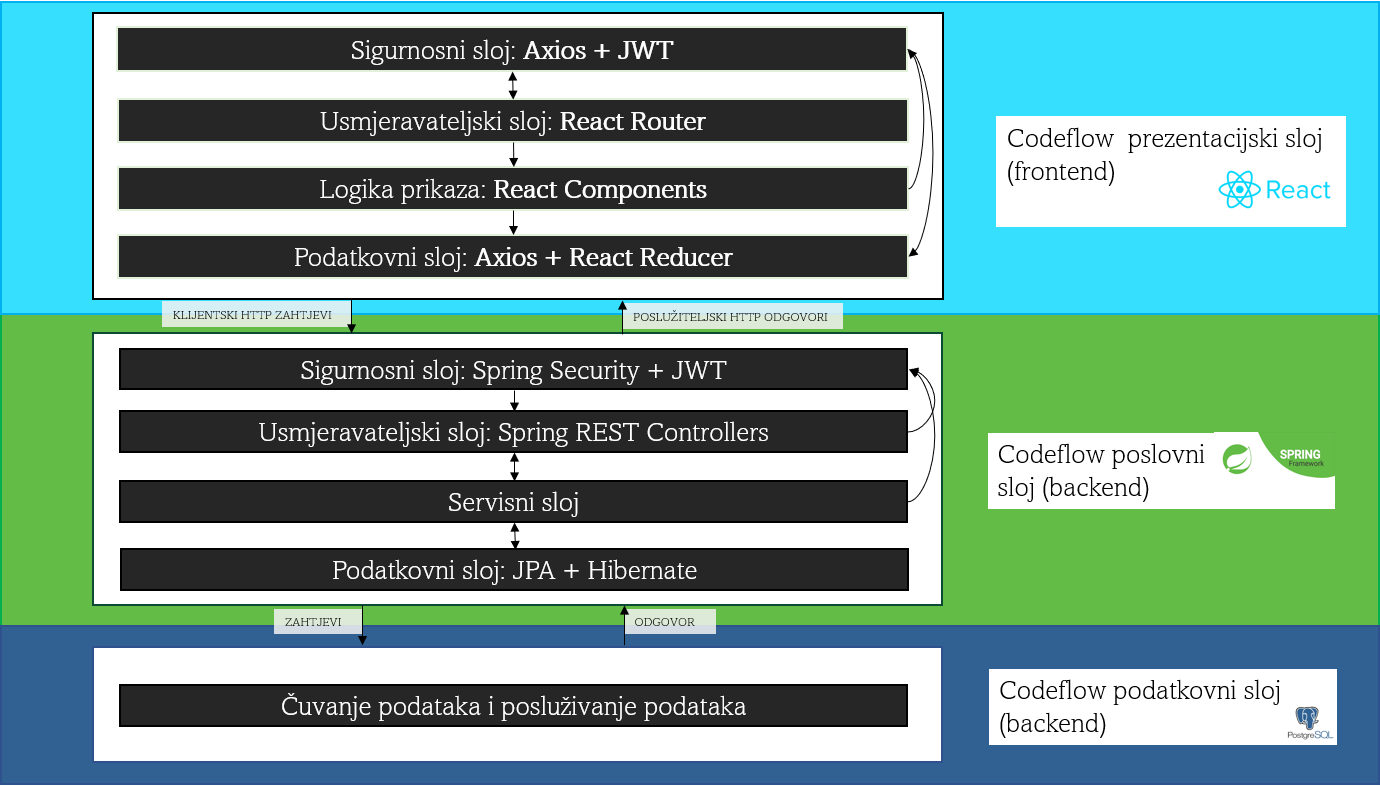
\includegraphics[width=\linewidth]{pictures/prikazi/Arhitektura.png}
			\caption{Arhitektura Codeflow aplikacije s naglašenim bitnijim tehnologijama i interakcijama svakog sloja.}
			\label{fig:arh}
		\end{figure}
	
			\subsubsection{Implementacija prezentacijskog sloja}
			Prezentacijski sloj definira korisničko sučelje aplikacije te je za njegovu izradu korišten React. React aplikacija prezentacijskog sloja sastoji se od jedanaest stranica od kojih svaka predstavlja određeni pogled definiran korisničkim zahtjevima, a same stranice koriste i dijele manje komponente. Radi bolje strukturiranog razvoja, React aplikacija dodatno je podijeljena je u četiri interna sloja: \textbf{sigurnosni sloj}, \textbf{usmjeravateljski sloj}, \textbf{sloj logike aplikacije} i \textbf{podatkovni sloj}.\\
			Korisnički zahtjevi razlikuju prijavljene i neprijavljene korisnike pa tako korisničko sučelje razlikuje i definira akcije dopuštene prijavljenim i neprijavljenim korisnicima. Tijekom uporabe, neprijavljeni korisnici isprva pristupaju \textbf{sigurnosnom sloju}. Sigurnosni sloj nakon uspješne prijave od poslovnog sloja dobiva dva \textit{http-only} kolačića \engl{cookie}. Oba sadržavaju \textit{JSON Web Tokens}\cite{jwt2021} (skraćeno JWT) i unutar sebe opisuju osnovne korisnikove podatke. Njihovim primitkom React aplikacija sigurna je da je korisnik uspješno ovjerio svoj identitet i da smije spremiti i koristiti njegove podatke.
		 	\textit{JSON Web Tokens} podijeljeni su u tri dijela: \textit{header} dio koji opisuje tip tokena i korišteni kriptografski algoritam, \textit{payload} dio koji sadržava korisničke informacije 
			i dio s potpisom koji je kriptirani sažetak prva dva dijela. Prvi kolačić šalje se uz svaki prijavljeni korisnički zahtjev, a drugi kolačić koristi se za obnovu prvog kolačića jer vremensko trajanje prvog kolačića vrlo je kratko (dvije minute). Odbijenost korisničkog zahtjeva zbog vremenskog isteka prvog kolačića ispravlja se pomoću \textit{Axios Response Interceptor} funkcionalnosti koja šalje novi zahtjev za obnovu kolačića. Novi zahtjev sadržava drugi kolačić. U slučaju odbijanja produljenja JWT kolačića korisnik se odjavljuje dok se u slučaju produljenja originalno odbijen zahtjev ponovno  šalje. Provjera ispravnosti poslanih kolačića obrađuje se unutar poslovnog sloja. Kombinacija JWT kolačića i provjere spremljenih podataka unutar lokalnog spremnika internetskog preglednika tijekom promjene stranica osiguravaju ispravno raspoznavanje prijavljenih korisnika i neprijavljenih korisnika.
			\begin{figure}[H]
				\centering
				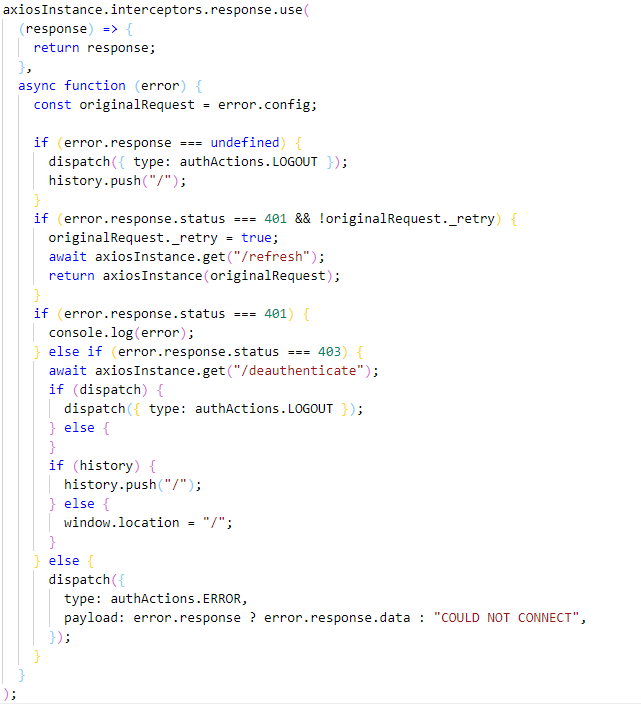
\includegraphics[scale=0.65]{pictures/prikazi/AxiosInterceptor.png}
				\caption{Primjer korištenja Axios Interceptor funkcionalnosti.}
				\label{fig:axiosinterceptor}
			\end{figure}
		
			\textbf{Usmjeravateljski sloj} koristi React Router tehnologiju koja (uz povratnu informaciju sigurnosnom sloju) preusmjerava korisnike na tražene stranice. \\
			Poslovna logika aplikacije definirana korisničkim zahtjevima obrađena je unutar \textbf{sloja logike aplikacije}. Sloj logike aplikacije uvelike koristi enkapsuliranu prirodu React komponenata. Svaka komponenta interno pohranjuje svoj izgled i funkcionalnost, a one variraju od posebnih gumbiju pa sve do tablica s rješenjima. Unutar ovog sloja zahtjevi usmjereni prema Judge0 izvršitelju slani su tijekom provjere korisničkog rješenja zadatka. \\
			U konačnici, \textbf{podatkovni sloj} koristi Axios biblioteku za slanje zahtjeva te React Reducer funkcionalnost Reacta za strukturirano spremanje i upravljanje podacima unutar React aplikacije.
			
	 		\subsubsection{Implementacija poslovnog sloja}
	 		Poslovni sloj Codeflow aplikacije sastoji se od internetskog poslužitelja pisanog Java programskim jezikom uz pomoć Spring radnog okvira. Arhitekturalni stil internetskog poslužitelja prilagođen je REST \engl{representational state transfer} arhitekturalnom stilu. Unutar REST arhitekturalnog stila, podaci i funkcionalnosti se smatraju resursima i pristupa im se pomoću URI-ja \engl{Uniform Resource Identifiers}. Sadržaj resursa može se oblikovati u različite medijske tipove, često zvane MIME \engl{Multipurpose Internet Mail Extensions}. Najčešći medijski tipovi sadržaja resursa su JSON \engl{Javascript Object Notation}, XML \engl{Extensible Markup Language} i HTML. REST također propisuje točno određene metode za pristup i modifikaciju resursa\cite{rest2021}.\\ Internetski poslužitelj, analogno prezentacijskom sloju, podijeljen je na interne slojeve radi kvalitetnije strukture. Slojevi po redu su: \textbf{sigurnosni sloj}, \textbf{usmjeravateljski sloj}, \textbf{servisni sloj} i \textbf{podatkovni sloj}. Semantički gledano, navedeni slojevi (izuzev sigurnosnog sloja) podliježu raspodjeli koju predlaže Spring radni okvir.\\
	 		Unutar \textbf{sigurnosnog sloja} dodan je poseban \textit{JwtFilter} koji služi za provjeru JWT kolačića spomenutih unutar implementacije prezentacijskog sloja. U slučaju neispravnog JWT kolačića unutar zahtjeva koji pristupa zaštićenom resursu, zahtjev biva odbijen i ne prosljeđuje se na usmjeravateljski sloj. JWT kolačić neispravan je ako je vremenski istekao ili ako se nanovo izračunati kriptografski sažetak, koji se računa  iz prva dva dijela tokena, ne podudara sa starim kriptografskim sažetkom zapisanim unutar dobivenog tokena. \textit{JwtFilter} ignorira zahtjeve za prijavu, registraciju i obnovu tokena, a uspješna prijava i obnova tokena generira nov par JWT kolačića pomoću \textbf{jjwt}\cite{jjwt2021} maven ovisnosti. Ista maven ovisnost koristi se i za provjeru tokena.
	 		\begin{figure}[H]
	 			\centering
	 			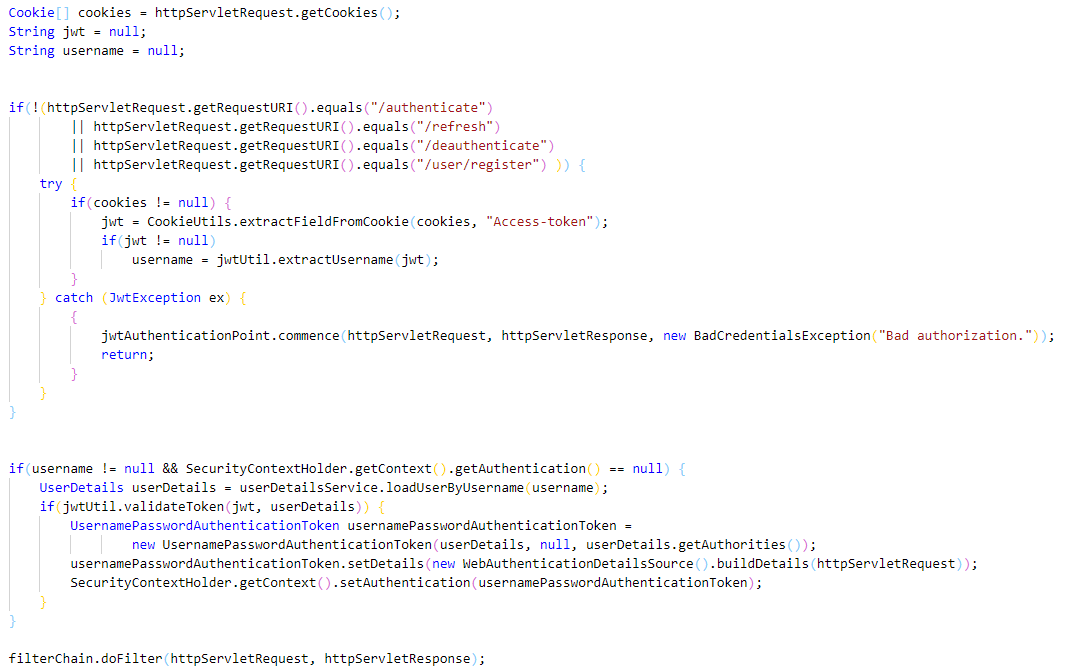
\includegraphics[width=\linewidth]{pictures/prikazi/JwtFilter.png}
	 			\caption{Programski kod JwtFiltera.}
	 			\label{fig:jwtfilter}
	 		\end{figure}
 		
	 		Ako zahtjev uspješno prođe sigurnosni sloj, stiže na \textbf{usmjeravateljski sloj} koji se sastoji od specijalnih REST Spring kontrolera koji Spring radnom okviru nalažu da vrijednost prilagodi JSON formatu i pospremi unutar tijela HTTP odgovora. Usmjeravateljski sloj sadržava kontroler za svaki od glavnih entiteta spomenutih unutar domene rješenja (\ref{sec:domenarjesenja}) te dodatni kontroler posvećen sigurnosti aplikacije. Kontroleri ne provode poslovnu logiku te pozivaju servisni sloj za daljnju obradu podataka. 
	 		\begin{figure}[H]
	 			\centering
	 			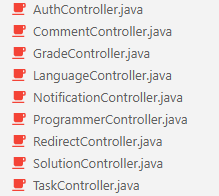
\includegraphics[scale=0.75]{pictures/prikazi/Controllers.png}
	 			\caption{Prikaz svih REST kontrolera usmjeravateljskog sloja.}
	 			\label{fig:controllers}
	 		\end{figure}
 		
	 		\textbf{Servisni sloj} sadržava servise unutar kojih se provodi poslovna logika diktirana korisničkim zahtjevima.
	 		\begin{figure}[H]
	 			\centering
	 			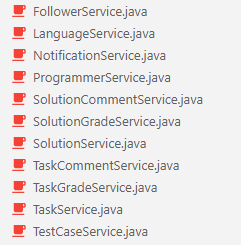
\includegraphics[scale=0.75]{pictures/prikazi/Services.png}
	 			\caption{Prikaz svih servisa servisnog sloja.}
	 			\label{fig:services}
	 		\end{figure}
 		
	 		\textbf{Podatkovni sloj} sastoji se od programskih klasa (znane još kao i model) koje opisuju entitete baze podataka te JPA repozitorijska \engl{repositories} sučelja. Repozitorijska sučelja interno unutar svojih implementacija provode prevođenje programskih naredbi u SQL naredbe te redaka dobivenih SQL upitima u objekte definiranih prigodnim modelom. Interna implementacija uvelike ovisi o Hibernate ORM radnom okviru. Podatkovni sloj poslovnog sloja jedini je sloj koji šalje zahtjeve bazi podataka.
			
			\subsubsection{Implementacija podatkovnog sloja}
			Podatkovni sloj sastoji se od PostgreSQL sustava za upravljanje bazama podataka. Omogućuje pohranjivanje i izmjenu podataka.
			
	\chapter{Evaluacija i rangiranje rješenja programskog zadatka}
	Provjeru točnosti rješenja programskog zadatka definiraju autori zadataka putem proizvoljnog broja ulazno-izlaznih parova. Za svaki par se provjerava vraća li program odgovarajući izlaz za zadani ulaz. Testni slučajevi unutar Codeflow aplikacije definirani su kao par ulaznih i izlaznih vrijednosti koji nikad ne mogu biti prazni. Sama provjera dobivene izlazne vrijednosti i očekivane vrijednosti delegirana je Judge0 izvršitelju programskog koda.\\
	\begin{figure}[H]
		\centering
		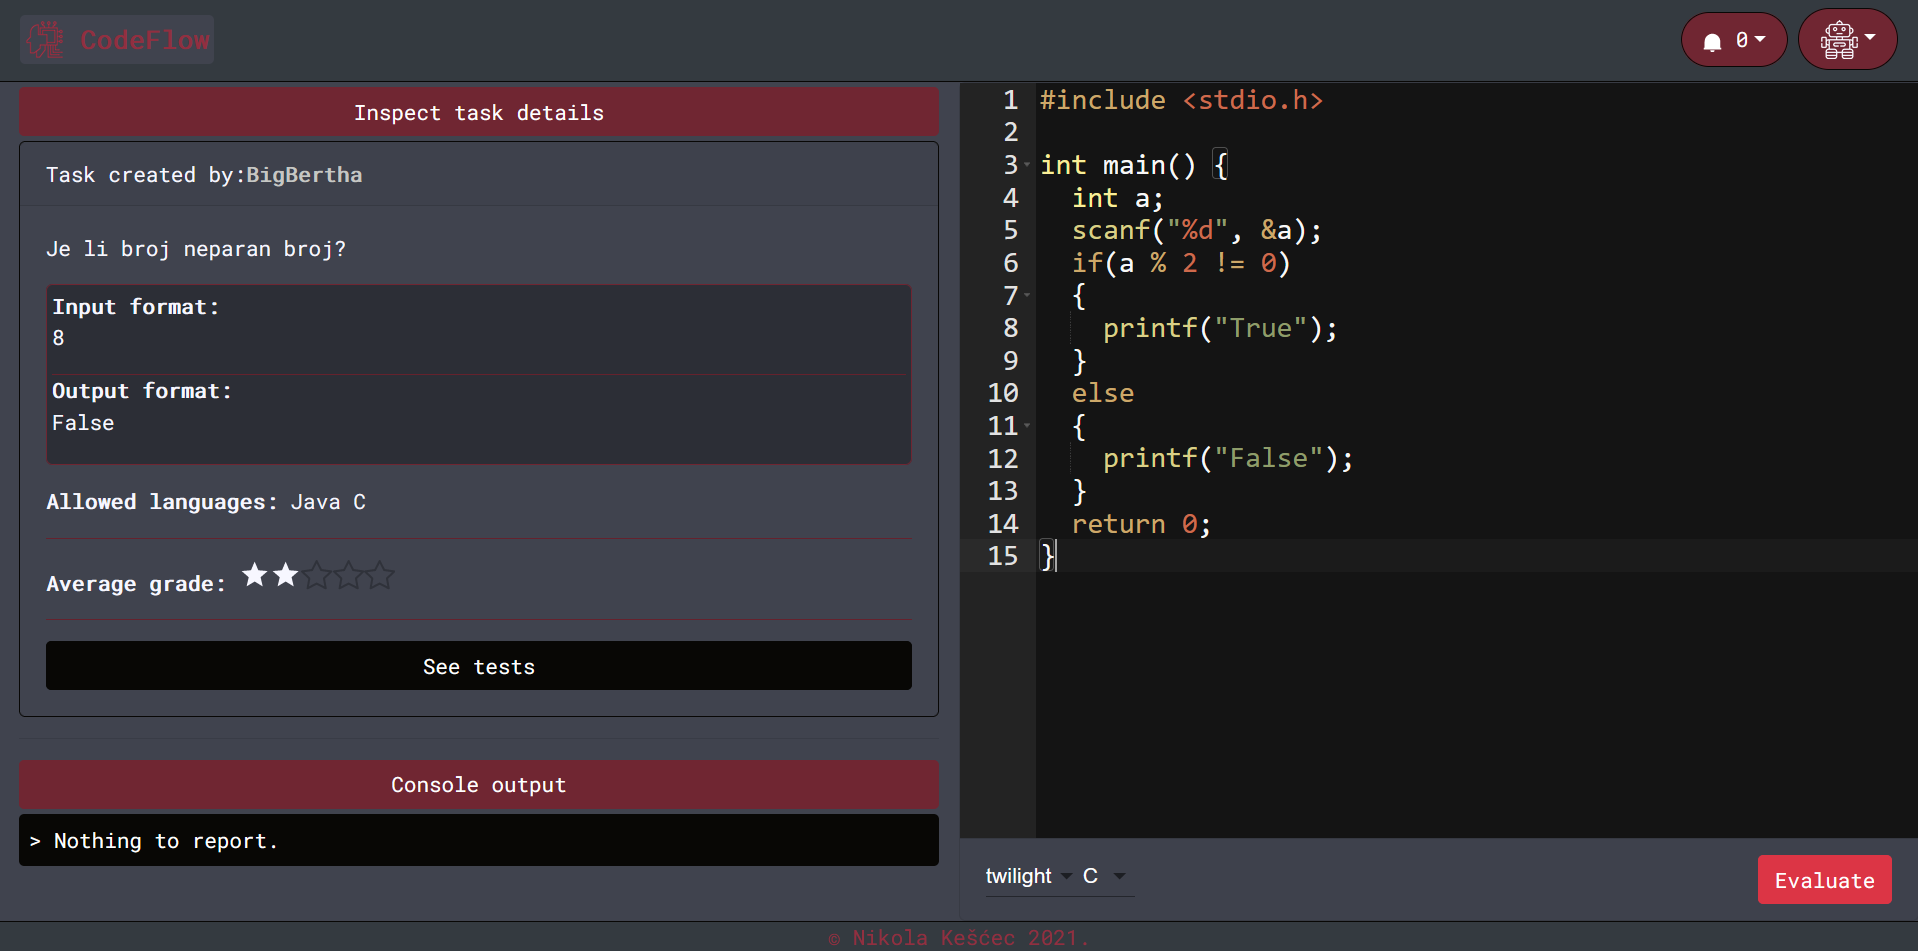
\includegraphics[width=\linewidth]{pictures/evaluacija/pocetak.png}
		\caption{Prikaz rješenja zadatka spremnog za evaluaciju. S lijeve strane unutar opisa zadatka vidljiv je primjer ulaznih i izlaznih testnih vrijednosti. Ispod detaljnog prikaza smješteno je područje koje ispisuje rezultate evaluacije.}
		\label{fig:start}
	\end{figure}
	Prvi korak evaluacije zadatka sastoji se od pripreme zahtjeva koji sadrži programski kod rješenja, identifikacijski broj programskog jezika rješenja, dio testnog slučaja koji definira ulaz te dio testnog slučaja koji definira očekivani izlaz rješenja. Pošto je zahtjev pripremljen, šalje se Judge0 izvršitelju programskog koda. Ako Judge0 uspješno prevede i izvede rješenje uspoređuje izlaz dobiven kao rezultat izvođenja programskog koda s očekivanim izlazom unutar tijela zahtjeva, inače vraća grešku. Nakon što aplikacija Codeflow zaprimi odgovor, pregledava tijelo odgovora. Ako tijelo odgovora sadržava obavijesti o bilo kakvim greškama nastalim tijekom prevođenja ili izvođenja, aplikacija grešku prikazuje korisniku te prestaje s daljnjom evaluacijom zadatka (prikazano na slici \ref{fig:error}).
	\begin{figure}[H]
		\centering
		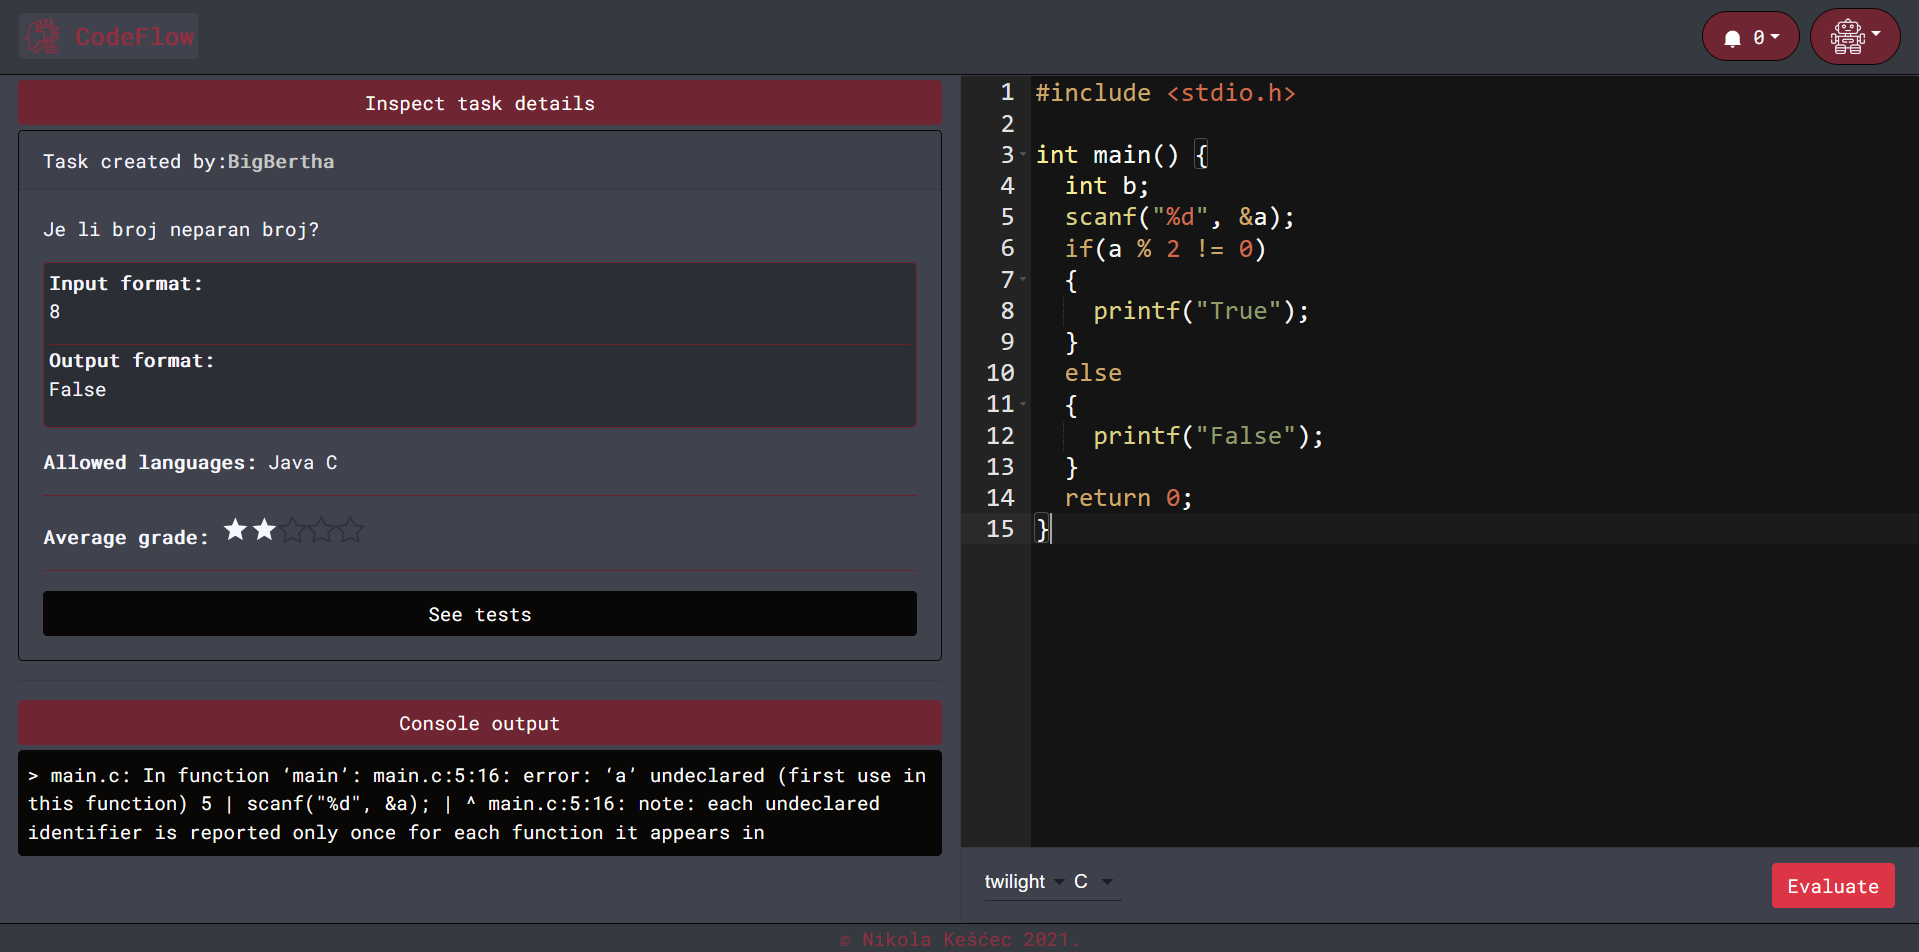
\includegraphics[width=\linewidth]{pictures/evaluacija/error.png}
		\caption{Prikaz rezultata evaluacije rješenja koje sadržava sintaksnu pogrešku.}
		\label{fig:error}
	\end{figure}
	Nadalje, ako se izlaz prevedenog i izvedenog rješenja ne podudara s očekivanim izlazom evaluacija se ne prekida, već se izvodi za sve dane ispitne slučajeve (nepodudarnosti se interno prate). Tek nakon izvođenja svakog od testnog slučaja bez grešaka korisnik biva obavješten o rezultatima podudarnosti dobivenih izlaza i očekivanih izlaza (prikaz je vidljiv na slici \ref{fig:badeval}).
	\begin{figure}[H]
		\centering
		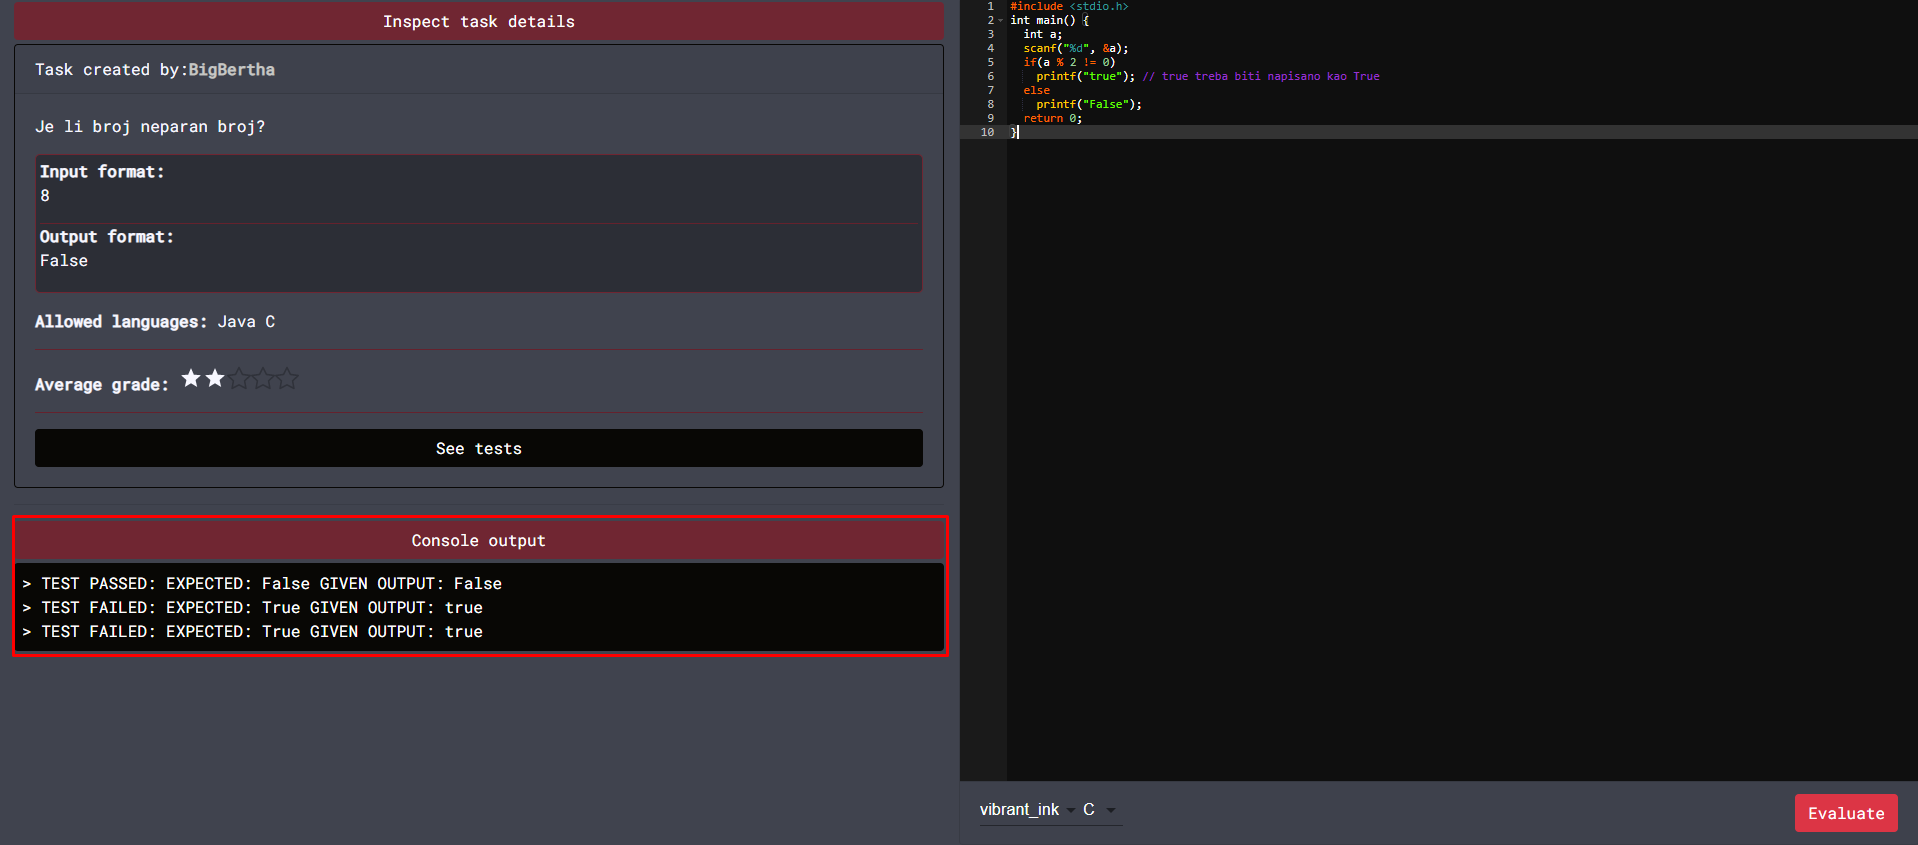
\includegraphics[width=\linewidth]{pictures/evaluacija/badeval.png}
		\caption{Prikaz evaluacije s nepodudaranjima. Naglašen je prostor rezultata usporedbe.}
		\label{fig:badeval}
	\end{figure} 
	Bitna napomena ovog sustava evaluacije jest da mogućnost spremanja rješenja programskog zadatka postaje dostupna samo u slučaju \textbf{potpune} podudarnosti svih dobivenih izlaza i očekivanih izlaza navedenih unutar testnih slučajeva. Prikaz uspješne evaluacije vidljiv je na slici \ref{fig:goodeval}. 
	\begin{figure}[H]
		\centering
		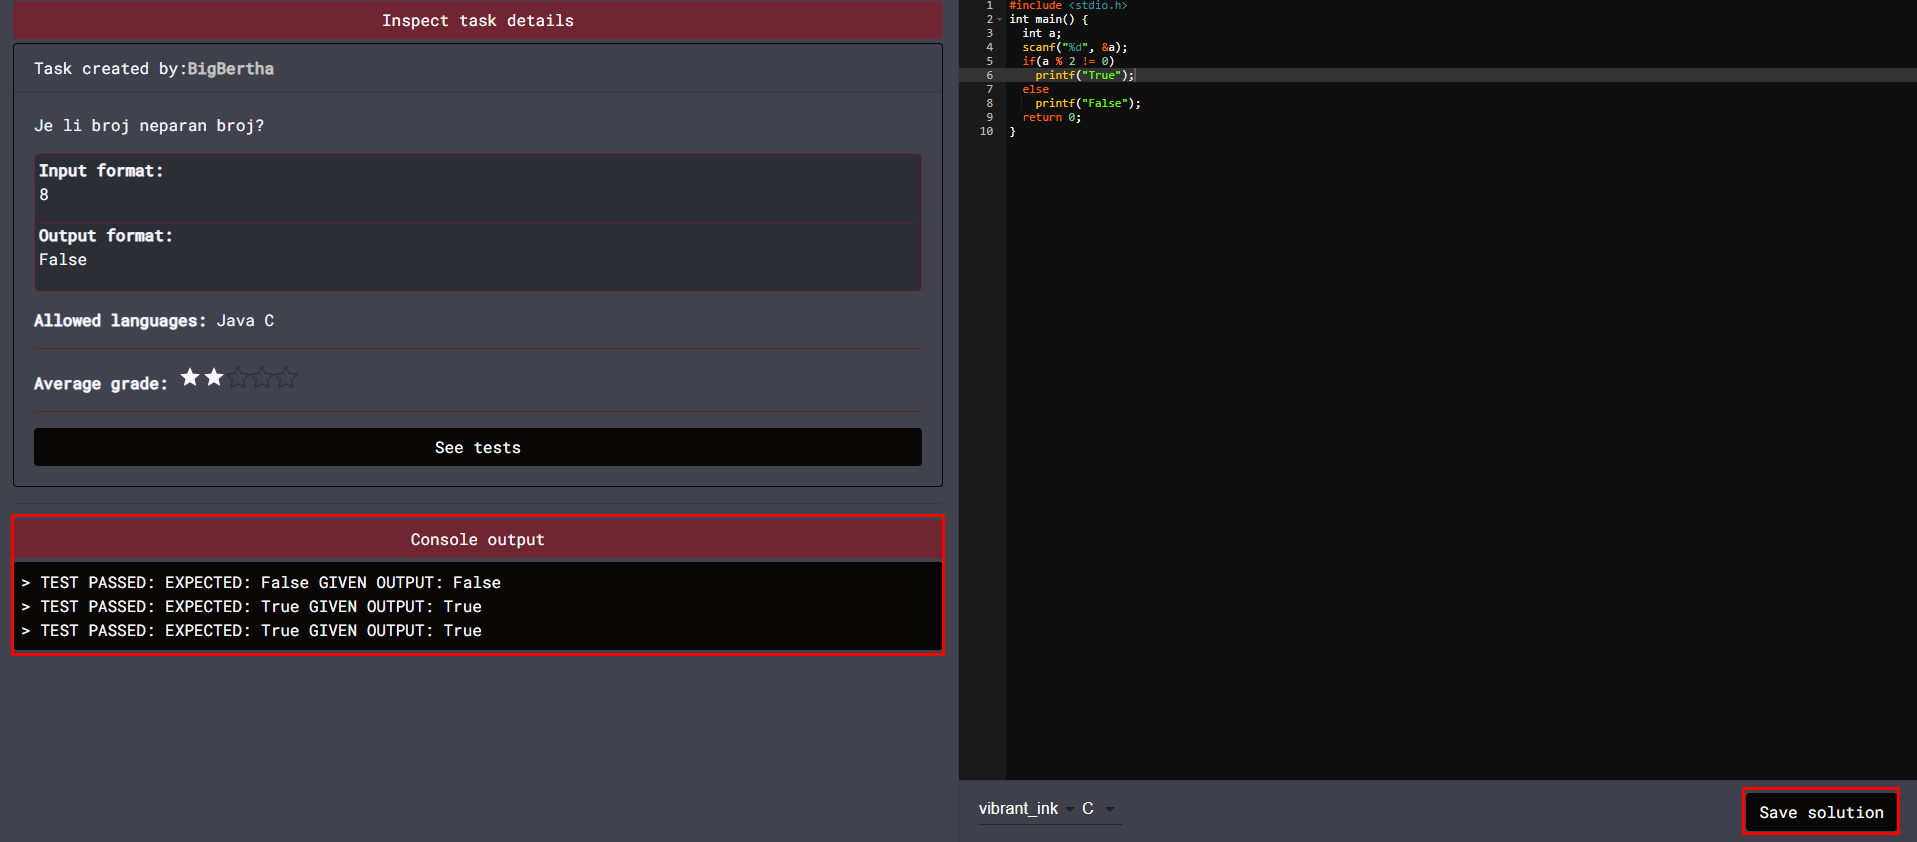
\includegraphics[width=\linewidth]{pictures/evaluacija/goodeval.png}
		\caption{Prikaz evaluacije s potpunim podudaranjem. Naglašen je prostor rezultata usporedbe i omogućeno spremanje rješenja zadatka.}
		\label{fig:goodeval}
	\end{figure}
	Grafički prikaz izvođenja evaluacije rješenja programskog zadatka unutar Codeflow aplikacije prikazan je na slici \ref{fig:algorithm}.
	\begin{figure}[H]
		\centering
		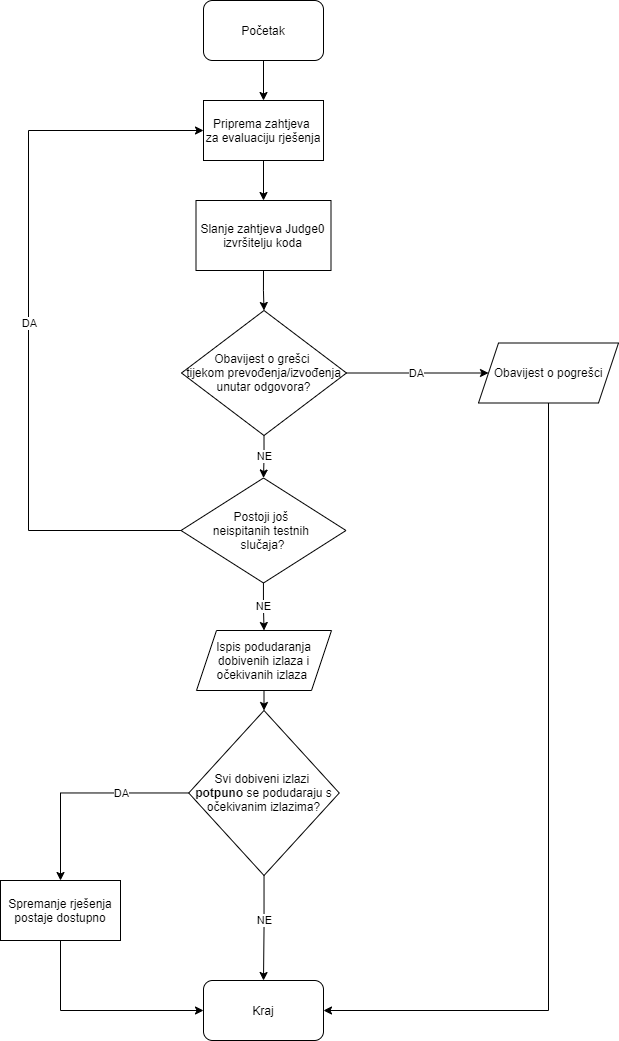
\includegraphics[width=\linewidth]{pictures/prikazi/Algorithm.png}
		\caption{Prikaz algoritma evaluacije rješenja zadatka unutar Codeflow aplikacije.}
		\label{fig:algorithm}
	\end{figure}
	Rangiranje rješenja provedeno je rangiranjem prosječne ocjene rješenja. Korisnici aplikacije ocjenjuju rješenja te se na temelju njihovih ocjena izračunava prosječna ocjena. Korisnici rješenje mogu ocijeniti samo jednom, a ako promijene svoje mišljenje u vezi dane ocjene, mogu ju izbrisati ili promijeniti. Pristup rangiranja prosječnom ocjenom odabran je zbog klijentske interakcije. Alternativan pristup rangiranja korisničkih rješenja bio bi na temelju trajanja izvršavanja rješenja, ali on nije odabran zbog nemogućnosti osiguravanja potpuno identičnih uvjeta tijekom izvođenja svakog korisničkog rješenja.
	
	\chapter{Primjer karakteristične korisničke uporabe}
	Ovo poglavlje posvećeno je razmatranju uporabe i ostvarenih funkcionalnosti Codeflow internetske aplikacije iz perspektive novog korisnika. Očekivani radni tok novog korisnika sastoji se od:
	\begin{enumerate}
		\item pregleda stranice dobrodošlice
		\item registracije
		\item prijave
		\item pregleda sažetaka zadataka
		\item praćenja korisnika
		\item prihvaćanja ili odbijanja zahtjeva za pratiteljstvo
		\item detaljnog pregleda zadatka (uz opcionalno komentiranje i uvjetovano ocjenjivanje)
		\item pregleda rješenja zadatka (uz opcionalno komentiranje i ocjenjivanje)
		\item rješavanja odabranog zadatka
		\item stvaranja zadatka
	\end{enumerate}

		\section{Pregled stranice dobrodošlice}
		Korisnici prvim pristupom Codeflow aplikaciji pregledavaju stranicu dobrodošlice. Ako nemaju korisnički račun, pritiskom na gumb \textit{Register} preusmjerava ih se na stranicu za registraciju.
		\begin{figure}[H]
			\centering
			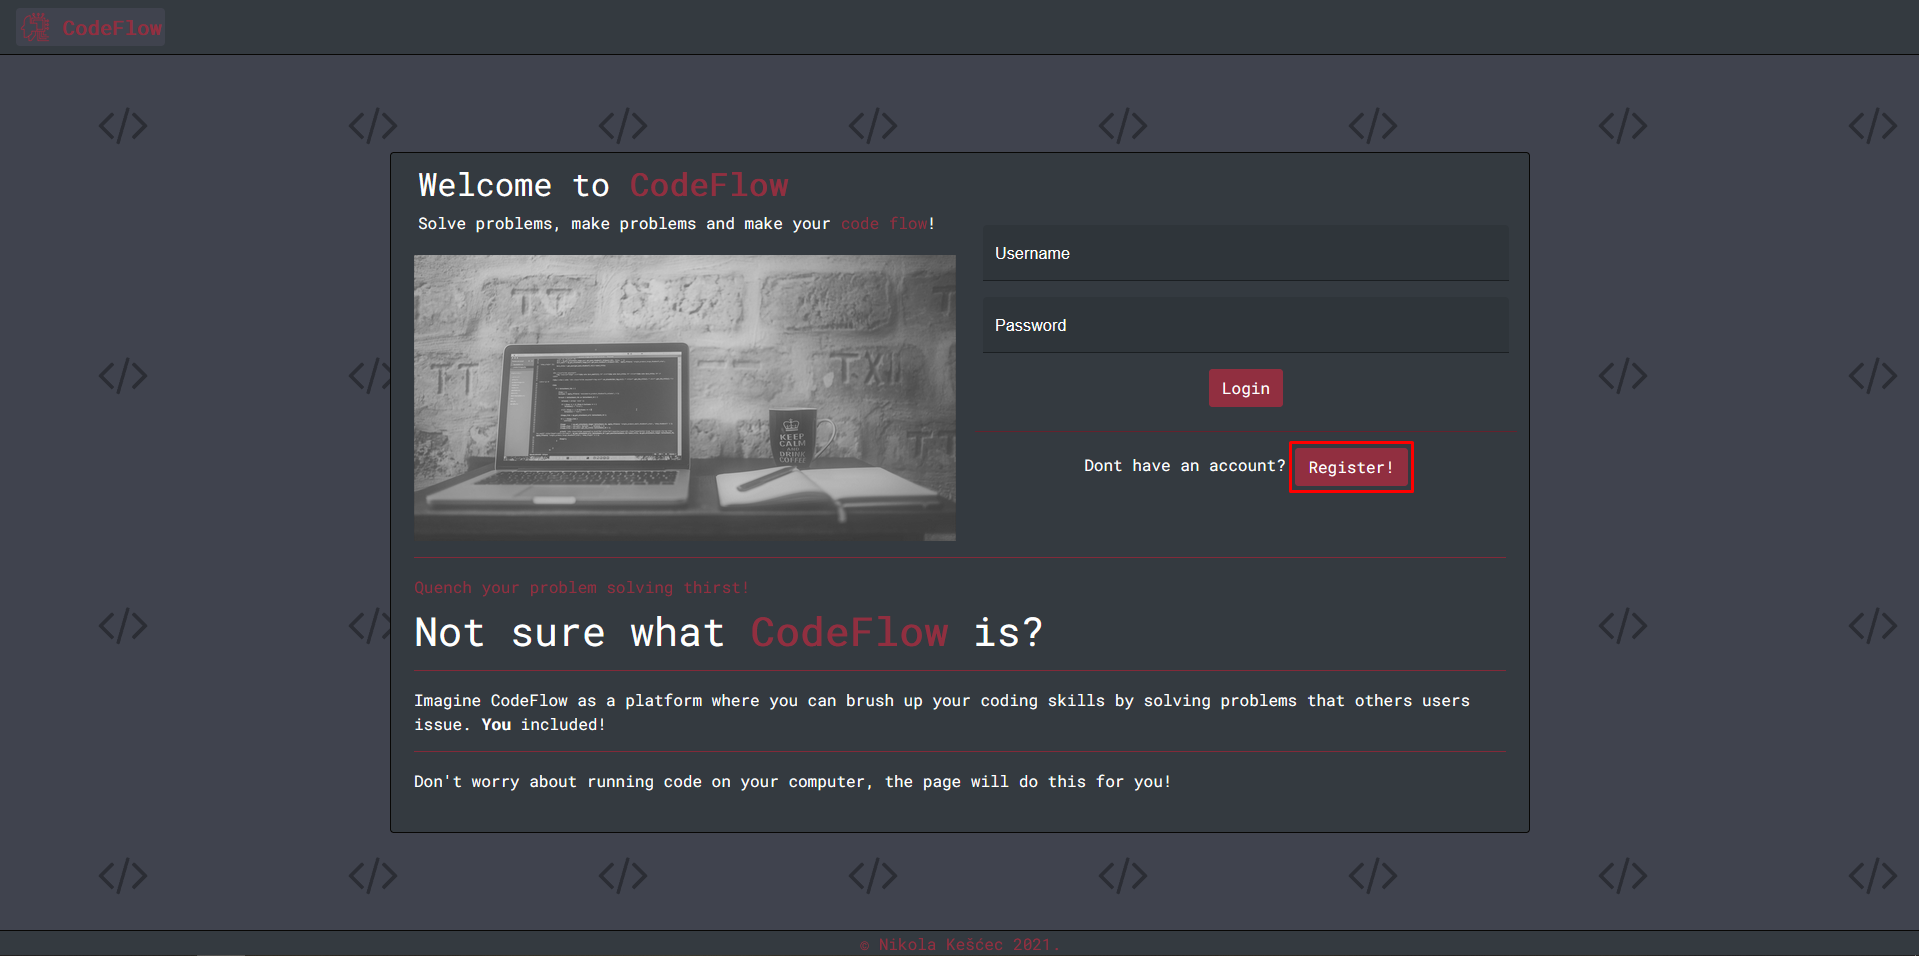
\includegraphics[width=\linewidth]{pictures/koristenje/StranicaDobrodoslice.png}
			\caption{Prikaz stranice dobrodošlice s naglašenim gumbom koji vodi na stranicu za registraciju.}
			\label{fig:welcome}
		\end{figure}
	
		\section{Registracija}
		Dolaskom na stranicu posvećenu registraciji korisnika neregistrirani korisnici moraju upisati podatke koji će se koristiti za stvaranje njihovog korisničkog računa. Polja za ispunu označena na slici \ref{fig:register} obavezna su te svako od njih sadržava dodatne uvjete. \textit{Username} i \textit{Email} polja moraju biti jedinstvena, \textit{Password} polje mora sadržavati lozinku dulju od 8 znakova te sadržaj \textit{Repeat your password} polja mora biti jednak \textit{Password} polju. Tek kada su navedeni uvjeti polja ispunjeni, korisnici pritiskom gumba \textit{Register} stvaraju novi korisnički račun s kojim se mogu prijaviti.
		\begin{figure}[H]
			\centering
			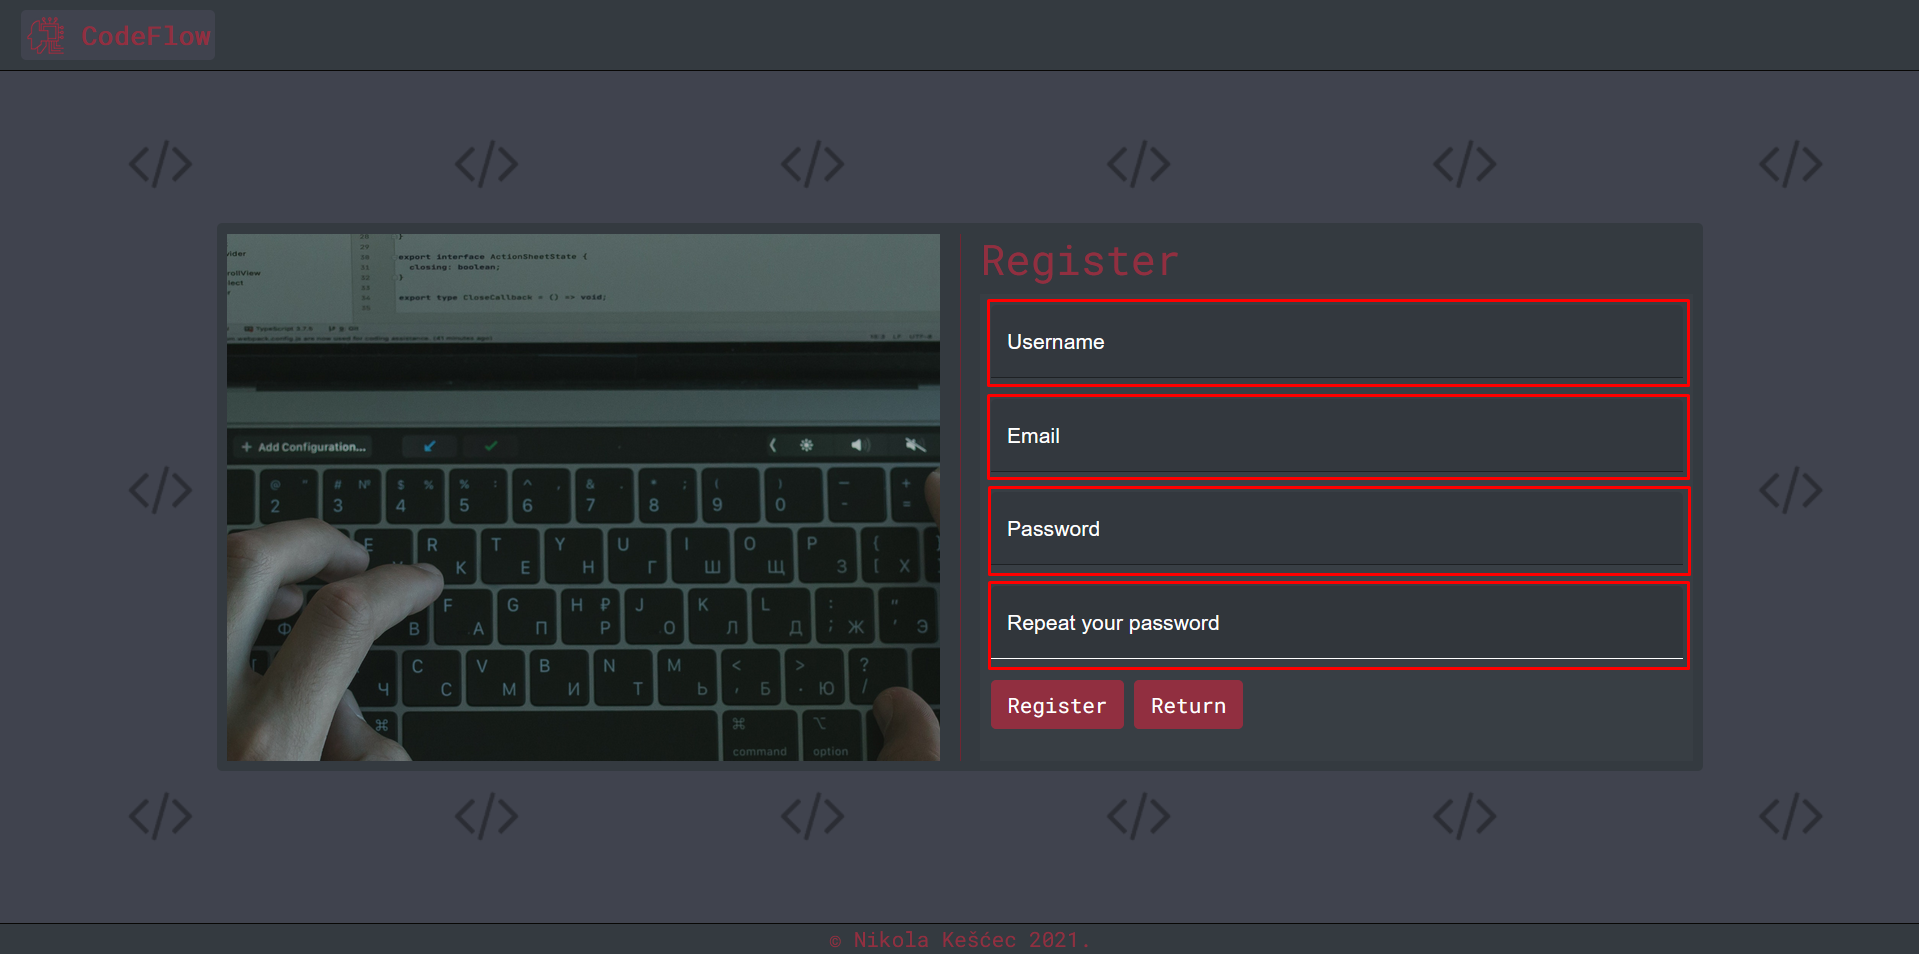
\includegraphics[width=\linewidth]{pictures/koristenje/Registracija.png}
			\caption{Prikaz stranice registracije s označenim elementima forme za prijavu.}
			\label{fig:register}
		\end{figure}
	
		\section{Prijava}
		Registrirani korisnici mogu se prijaviti pomoću podataka koje su tijekom registracije definirali. Podaci koji su relevantni za prijavu su \textit{Username} i \textit{Password} (vidljivi na slici \ref{fig:welcome}). Ako tijekom prijave bilo koji od tih podataka nije ispravan, Codeflow aplikacija će obavijestiti korisnika o pogrešci, ali neće naglasiti koji od podataka nije točan (iz sigurnosnih razloga).
	
		\section{Pregled sažetaka zadataka}
		\label{sec:sazetak}
		Nakon prijave, korisnici mogu pregledavati ponuđene sažetke zadataka. Sažetak zadatka sadržava opis zadatka, korisničko ime autora zadatka i prosječnu ocjenu zadatka. Ponuđene sažetke korisnici mogu filtrirati prema \textit{Recommended}, \textit{Following} i  \textit{Fresh} opcijama. \textit{Recommended} je prva opcija i ona predlaže korisnicima samo sažetke zadataka čiji su autori korisnici koje prijavljeni korisnici prate te sažetke zadataka s prosječnom ocjenom većom od određenog praga. Druga, \textit{Following} opcija, isto tako prikazuje isključivo sažetke zadataka čiji su autori korisnici koje prijavljeni korisnici prate. Treća, \textit{Fresh} opcija, prikazuje sažetke zadataka prema njihovoj starosti. Stranica s filtriranim sažetcima zadataka nije jedina stranica gdje je moguće vidjeti sažetke zadataka jer korisnici mogu pregledavati sažetke zadataka pojedinačnih korisnika na njihovim korisničkim stranicama. Do pojedinačnih korisničkih stranica dolazi se pritiskom na odabrano korisničko ime (strelicom naznačeno na slici \ref{fig:pregled}).
		\begin{figure}[H]
			\centering
			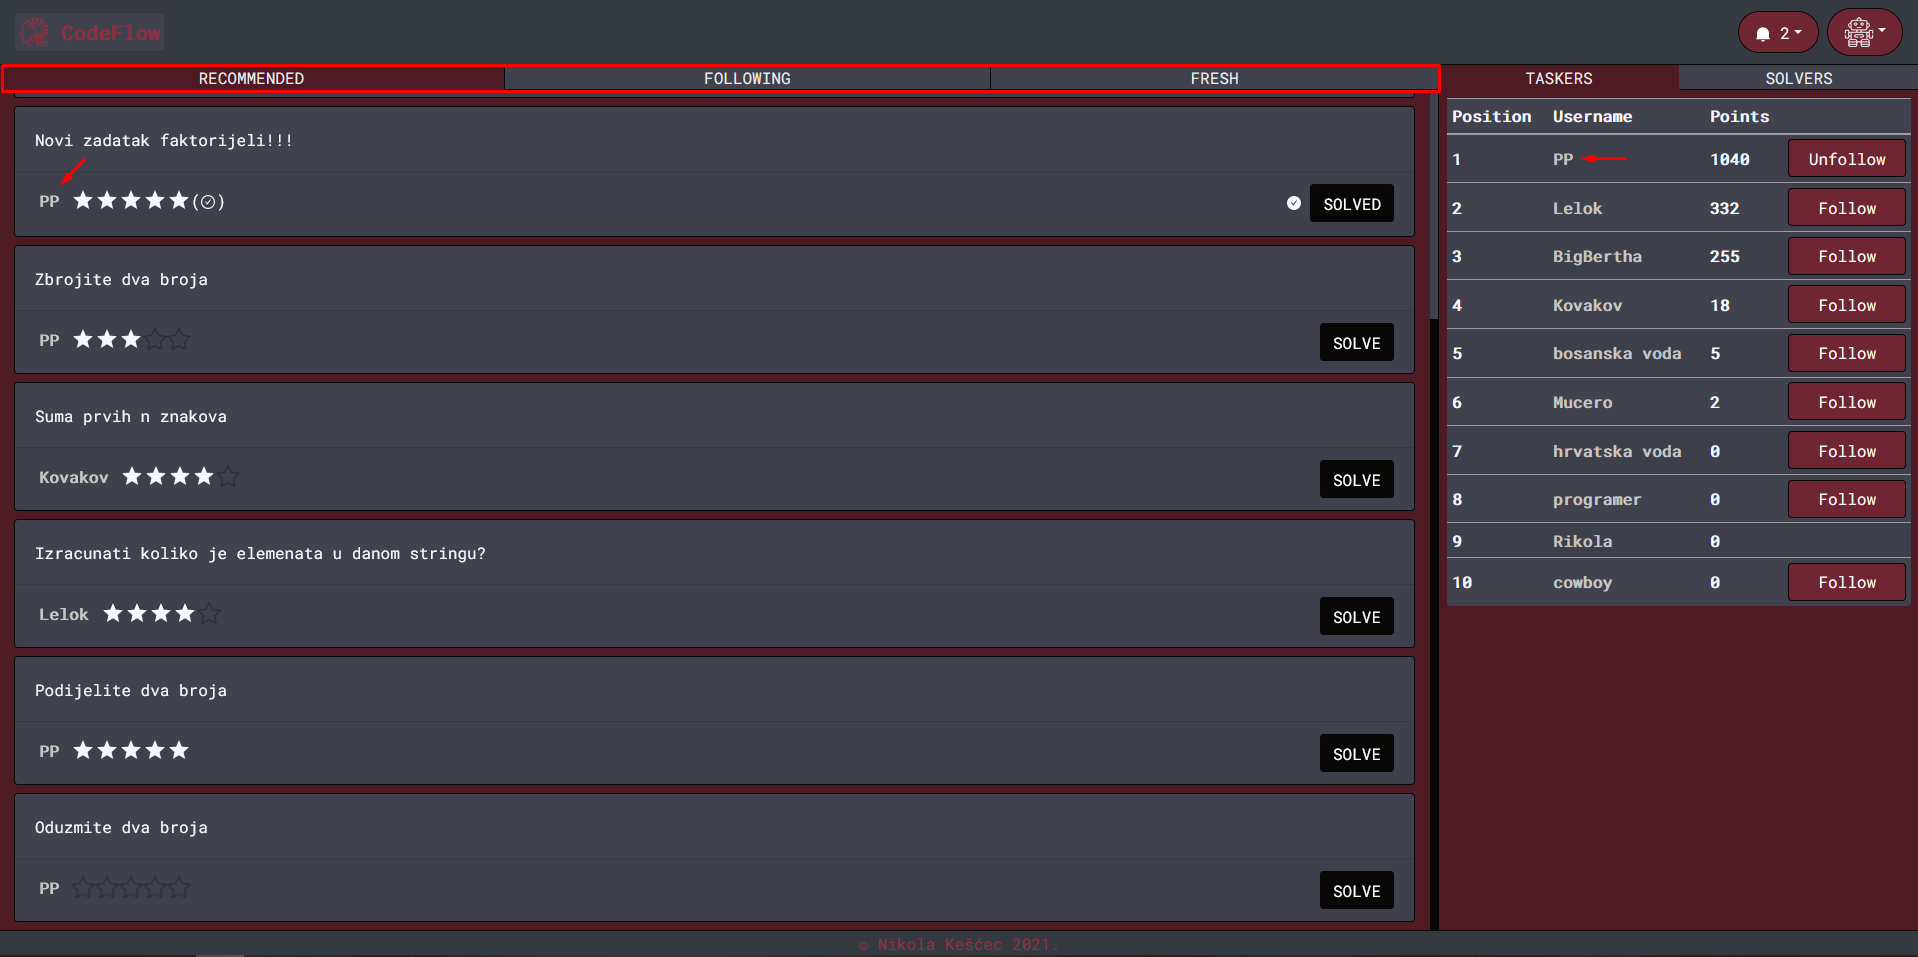
\includegraphics[width=\linewidth]{pictures/koristenje/Pregled.png}
			\caption{Prikaz stranice s mogućnošću pregleda i filtriranja ponuđenih sažetaka zadataka te naznačenim imenom korisnika koje vodi do korisničke stranice tog korisnika.}
			\label{fig:pregled}
		\end{figure}
	
		\section{Praćenje korisnika}
		Korisnici Codeflow aplikacije imaju mogućnost praćenja drugih korisnika. Zahtjev za praćenjem može se predati na dva načina: direktnim pritiskom na gumb \textit{Follow} unutar rang tablice korisnika (kao što je označeno na slici \ref{fig:pracenje1}) ili direktnim odlaskom na korisničku stranicu određenog korisnika (istim mehanizmom kao i kod pregleda sažetaka zadataka pojedinog korisnika). Na korisničkoj stranici pritiskom gumba \textit{Follow} ostvaruje se ista funkcionalnost kao i u prvom navedenom načinu. Klikom na gumb Follow samo se šalje zahtjev za pratiteljstvo koje onda korisnik kojem je usmjereno pratiteljstvo mora odobriti ili odbaciti.
		\begin{figure}[H]
			\centering
			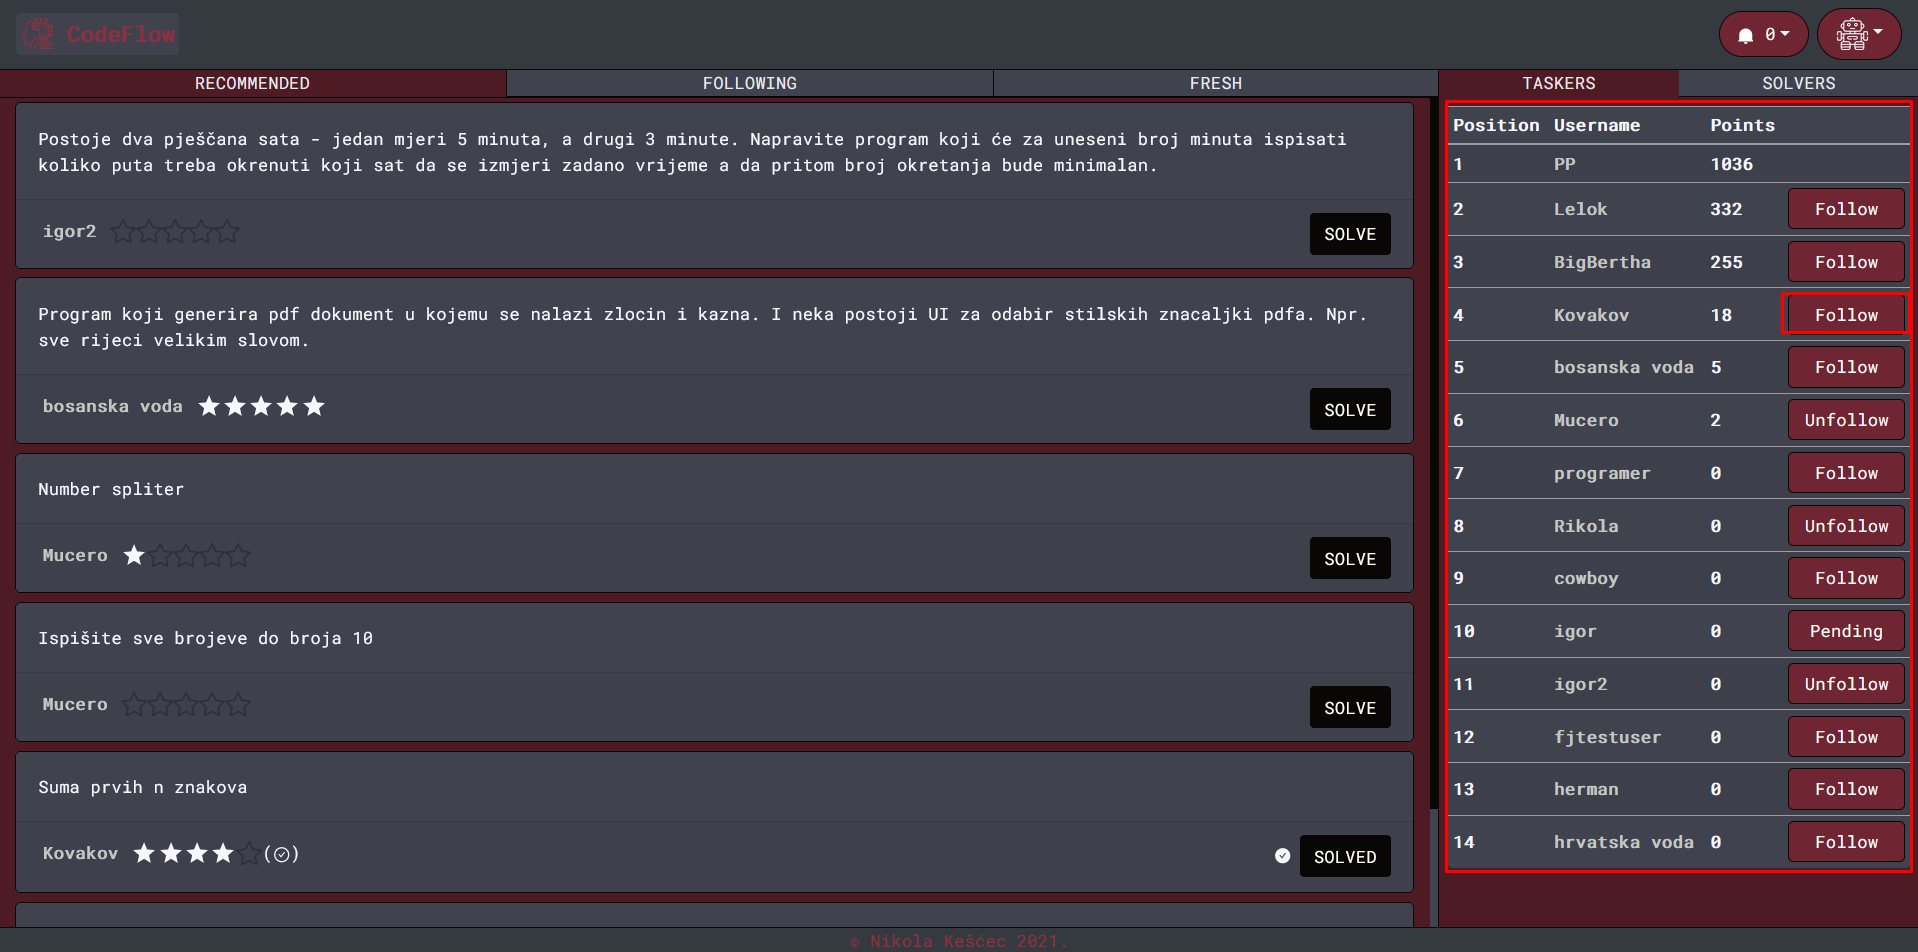
\includegraphics[width=\linewidth]{pictures/koristenje/Pracenje1.png}
			\caption{Prikaz stranice s prvim naglašenim načinom praćenja korisnika.}
			\label{fig:pracenje1}
		\end{figure}
		\begin{figure}[H]
			\centering
			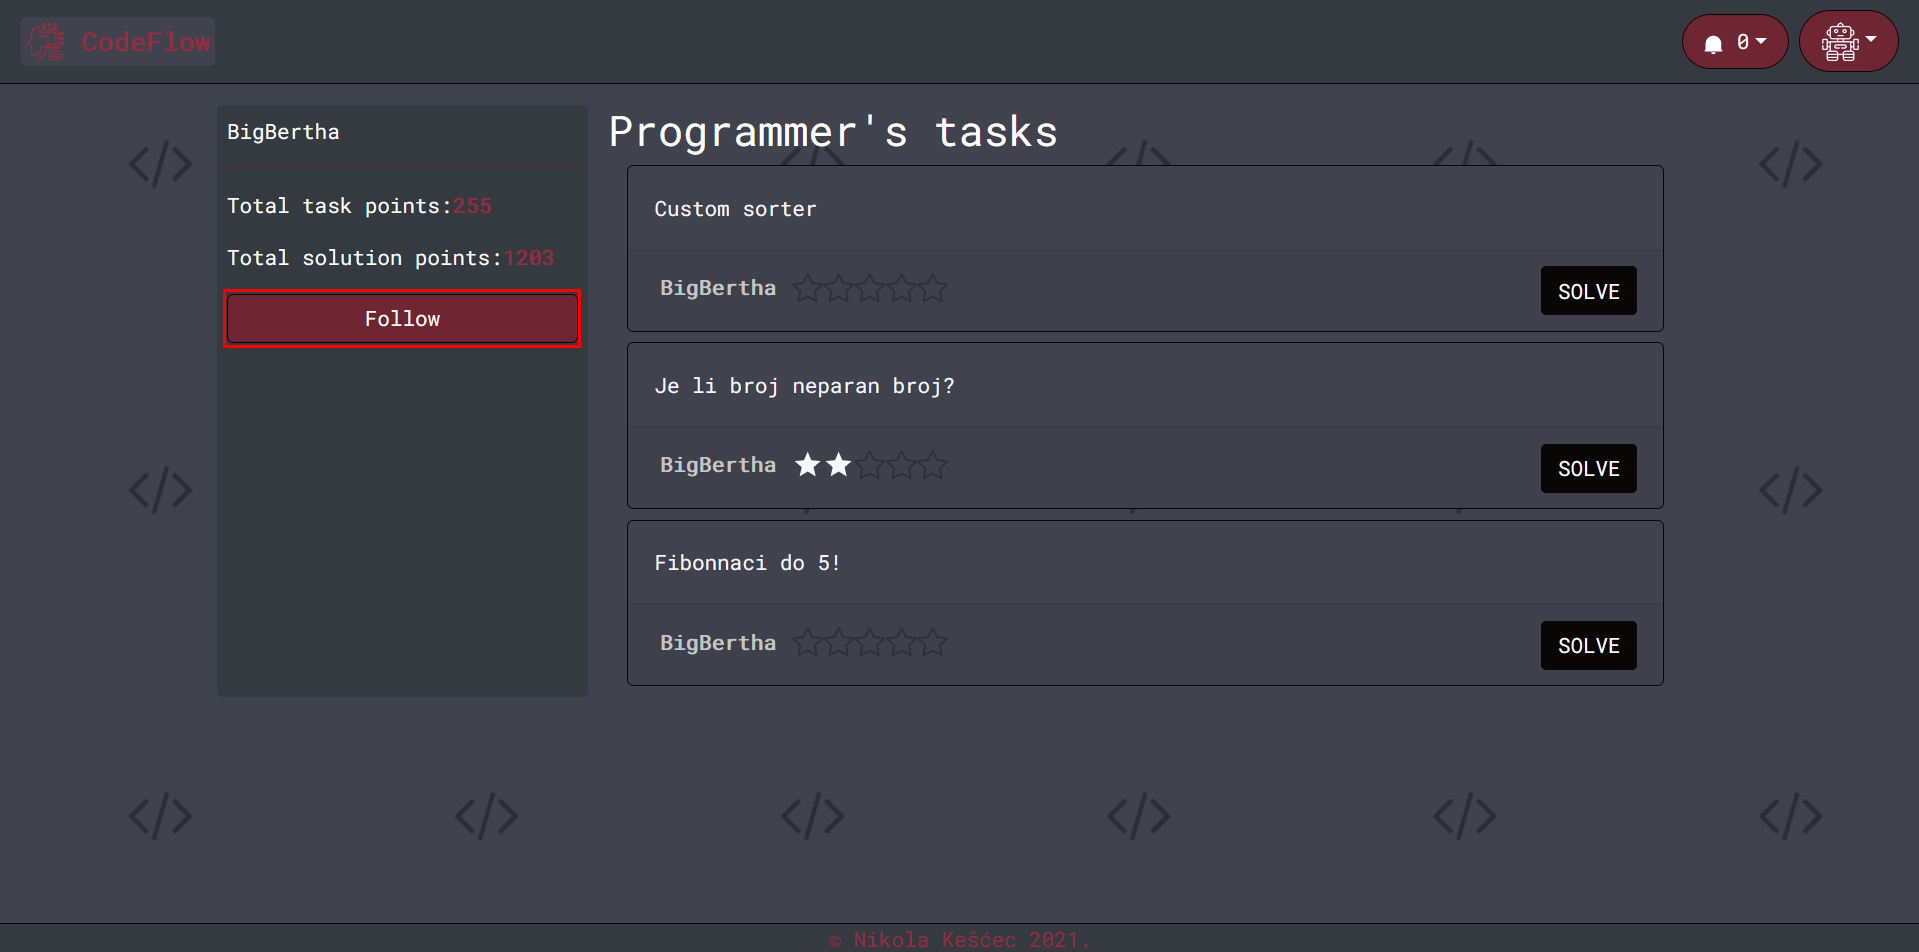
\includegraphics[width=\linewidth]{pictures/koristenje/Pracenje2.png}
			\caption{Prikaz stranice drugog korisnika s naglašenim gumbom za praćenje.}
			\label{fig:pracenje2}
		\end{figure}
	
		\section{Prihvaćanje ili odbijanje zahtjeva za pratiteljstvo}
		Zahtjev za prijateljstvo korisnici mogu prihvatiti ili odbiti. Svaki od zahtjeva formiran je u obliku obavijesti. Sve obavijesti korisnici u bilo kojem trenutku korištenja Codeflow aplikacije (ako postoje) mogu pregledati klikom na \textit{dropdown} gumb označen na slici \ref{fig:notificationbutton}. Pritiskom na taj gumb sve dostupne obavijesti korisnicima su prikazane te korisnici unutar obavijesti koje sadržavaju zahtjeve za pratiteljstvo imaju pravo navedeni zahtjev prihvatiti ili odbiti.
		\begin{figure}[H]
			\centering
			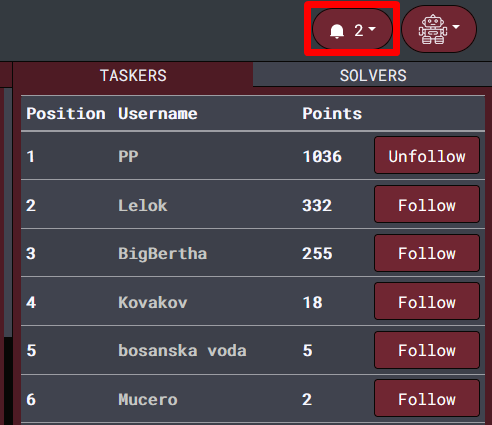
\includegraphics[scale=0.65]{pictures/koristenje/GumbZaObavijesti.png}
			\caption{Prikaz izgleda \textit{dropdown} gumba s obavijestima.}
			\label{fig:notificationbutton}
		\end{figure}
		\begin{figure}[H]
			\centering
			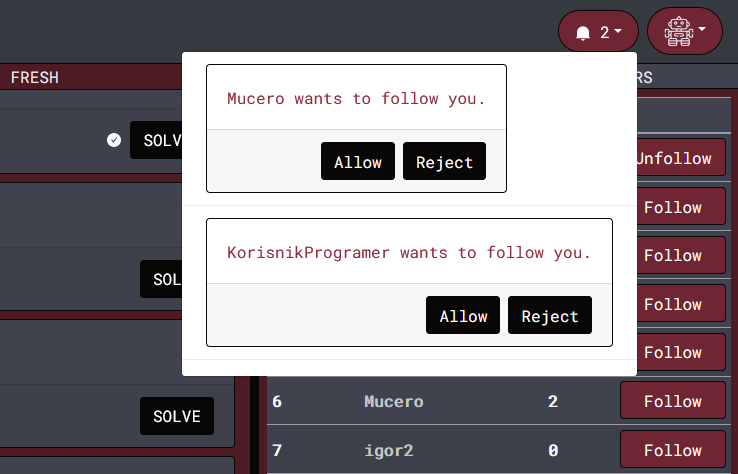
\includegraphics[scale=0.55]{pictures/koristenje/ZahtjevObavijesti.png}
			\caption{Prikaz obavijesti koje sadržavaju zahtjeve za pratiteljstvo.}
			\label{fig:pratiteljstvo}
		\end{figure}
	
		\section{Detaljan pregled zadatka (uz opcionalno komentiranje i ocjenjivanje)}
		Detaljan pregled zadatka korisnici mogu obaviti pritiskom gumbiju \textit{SOLVE} (ako nije već riješio), \textit{SOLVED} (ako je već riješio) ili \textit{INSPECT} (ako je rješenje njegovo). Gumb koji vodi na detaljan pregled zadatka nalazi se na sažetku zadatka spomenutog tijekom objašnjavanja pregleda sažetaka zadataka (\ref{sec:sazetak}). Stranica koja prikazuje detaljan pregled zadatka sadržava ime autora, opis zadatka, primjer upisa i ispisa, dopuštene programske jezike rješenja zadataka te prosječnu ocjenu. Opcionalno, korisnici mogu komentirati zadatak pisanjem komentara unutar polja za pisanje komentara (naznačeno na slici \ref{fig:detaljanpregled}). Ocjenjivanje zadatka korisnicima je moguće tek nakon rješavanja zadatka.
		\begin{figure}[H]
			\centering
			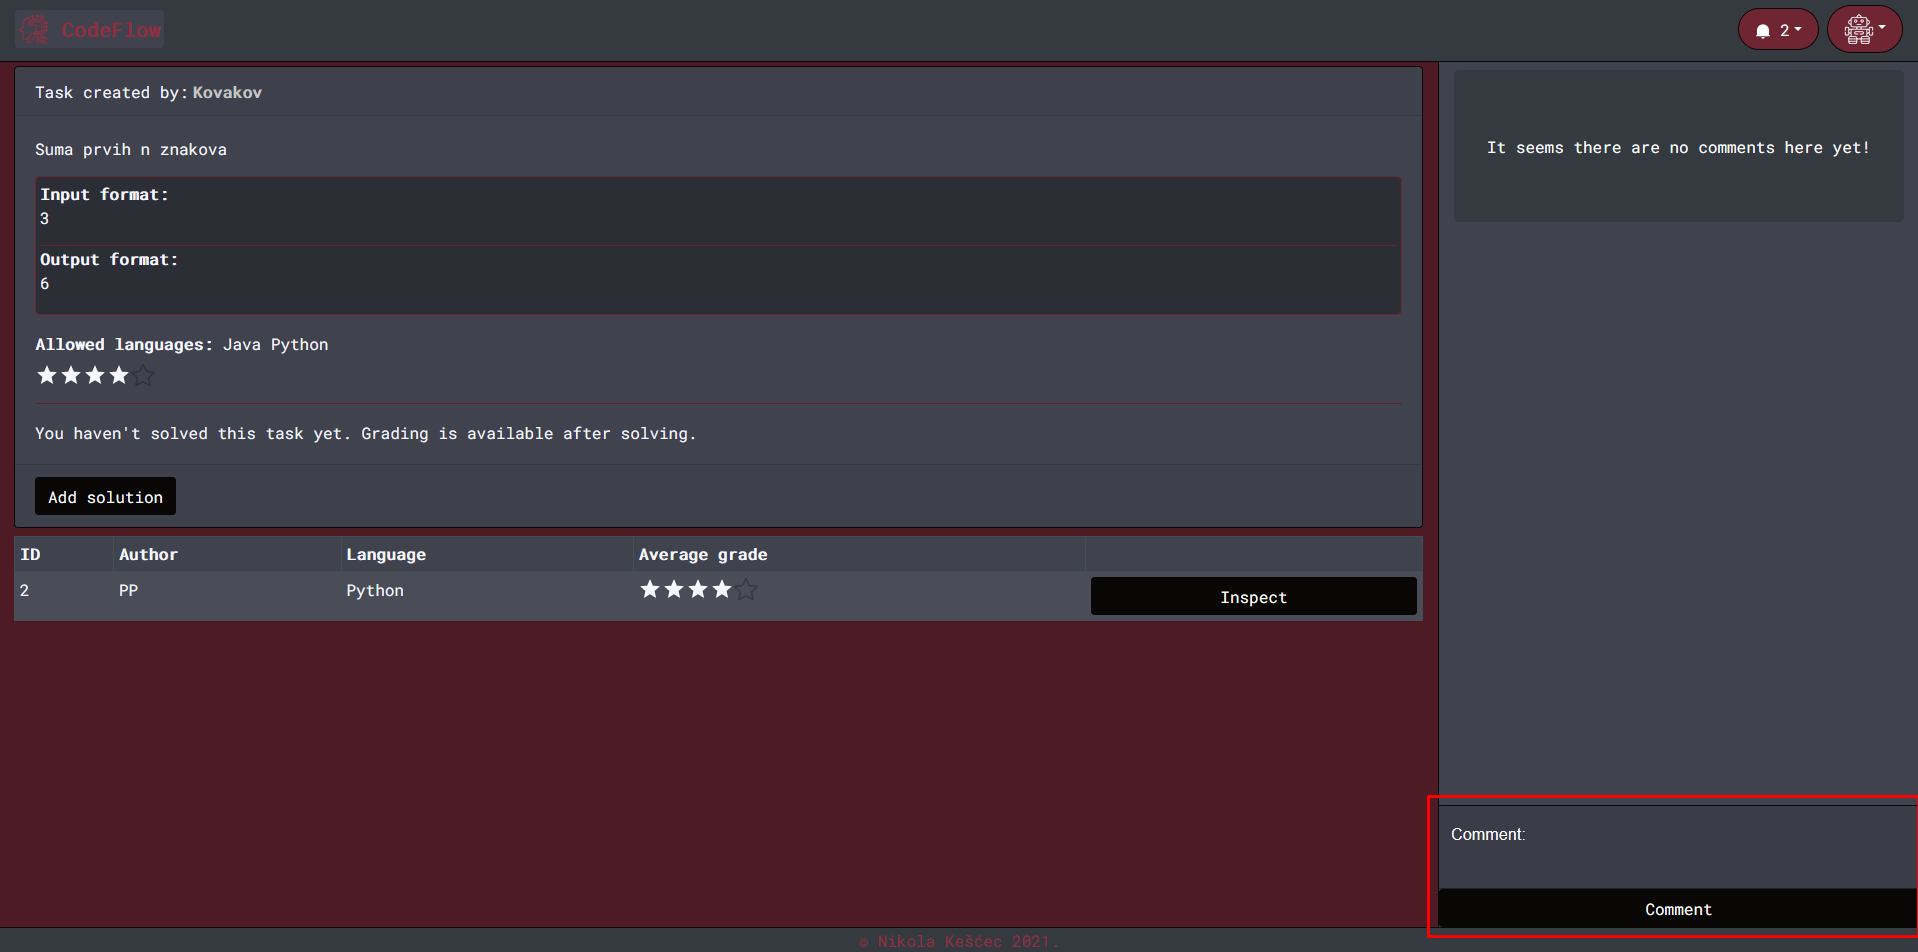
\includegraphics[width=\linewidth]{pictures/koristenje/DetaljanPregledZadatka.png}
			\caption{Prikaz detaljnog pregleda zadatka s naglašenim prostorom za unos opcionalnog komentara.}
			\label{fig:detaljanpregled}
		\end{figure}
	
		\section{Pregled rješenja zadatka (uz opcionalno komentiranje i ocjenjivanje)}
		Detaljan pregled rješenja zadatka korisnici mogu obaviti pritiskom gumba \textit{Inspect} unutar tablice rješenja koja se nalazi na detaljnom pregledu zadatka. Stranica koja prikazuje detaljan pregled zadatka sadržava ime autora, programski jezik rješenja, programski kod rješenja te prosječnu ocjenu. Opcionalno, korisnici mogu komentirati zadatak pisanjem komentara unutar polja za pisanje komentara (postupak je identičan kao i kod komentiranja zadatka). Također, korisnici uz opcionalno komentiranje rješenja mogu i ocijeniti rješenje ocjenom od 1 do 5.
		\begin{figure}[H]
			\centering
			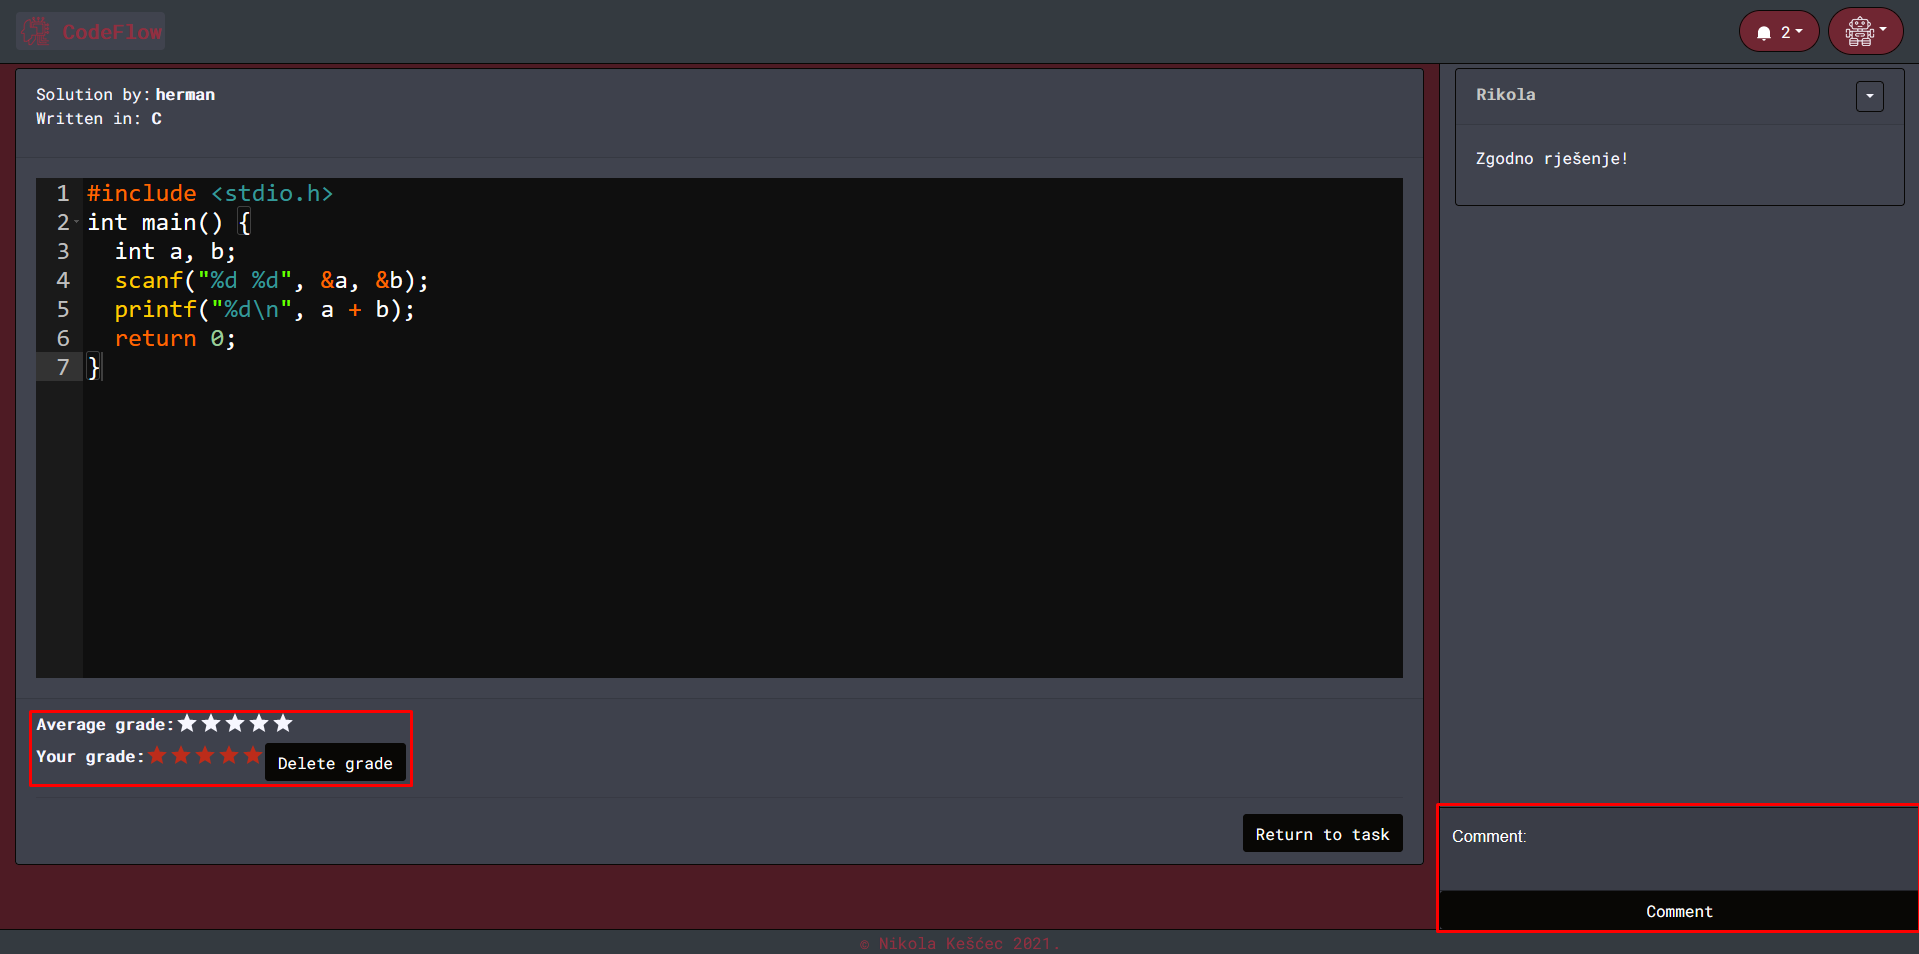
\includegraphics[width=\linewidth]{pictures/koristenje/PregledRjesenja.png}
			\caption{Prikaz pregleda rješenja zadatka uz naglašene elemente opcionalnog ocjenjivanja te komentiranja.}
			\label{fig:pregledrjesenje}
		\end{figure}
	
		\section{Rješavanje odabranog zadatka}
		Tijekom detaljnog pregleda zadatka korisnici imaju mogućnost riješiti zadatak pritiskom na gumb \textit{Add solution}. U slučaju da je korisnik već riješio zadatak gumb \textit{Inspect my solution} bit će prikazan umjesto \textit{Add solution} gumba te će taj gumb korisnika voditi na stranicu pregleda njegovog rješenja. Pošto korisnici pritisnu gumb \textit{Add solution} bit će odvedeni na stranicu koja sadržava detalje zadatka, izlaz konzole i uređivač programskog koda. Detalji zadatka navedeni su istim redom kao i na detaljnom prikazu rješenja uz nadodanu mogućnost pregledavanja testova. Tijekom rješavanja zadatka korisnici mogu mijenjati temu uređivača programskog koda te programski kod u kojem pišu rješenje (svaki zadatak definira dopuštene programske jezike). Pošto korisnici napišu rješenje, pritisak na \textit{Evaluate} gumb prvo će rješenje poslati na provjeru Judge0 izvršitelju programskog koda, a tek nakon uspješne usporedbe izlaza programskog rješenja s testovima zadatka bit će omogućeno spremanje rješenja zadatka pritiskom na gumb \textit{Save solution}. Nakon spremanja zadatka korisnici će biti preusmjereni na pregled njihovog rješenja zadatka.
		\begin{figure}[H]
			\centering
			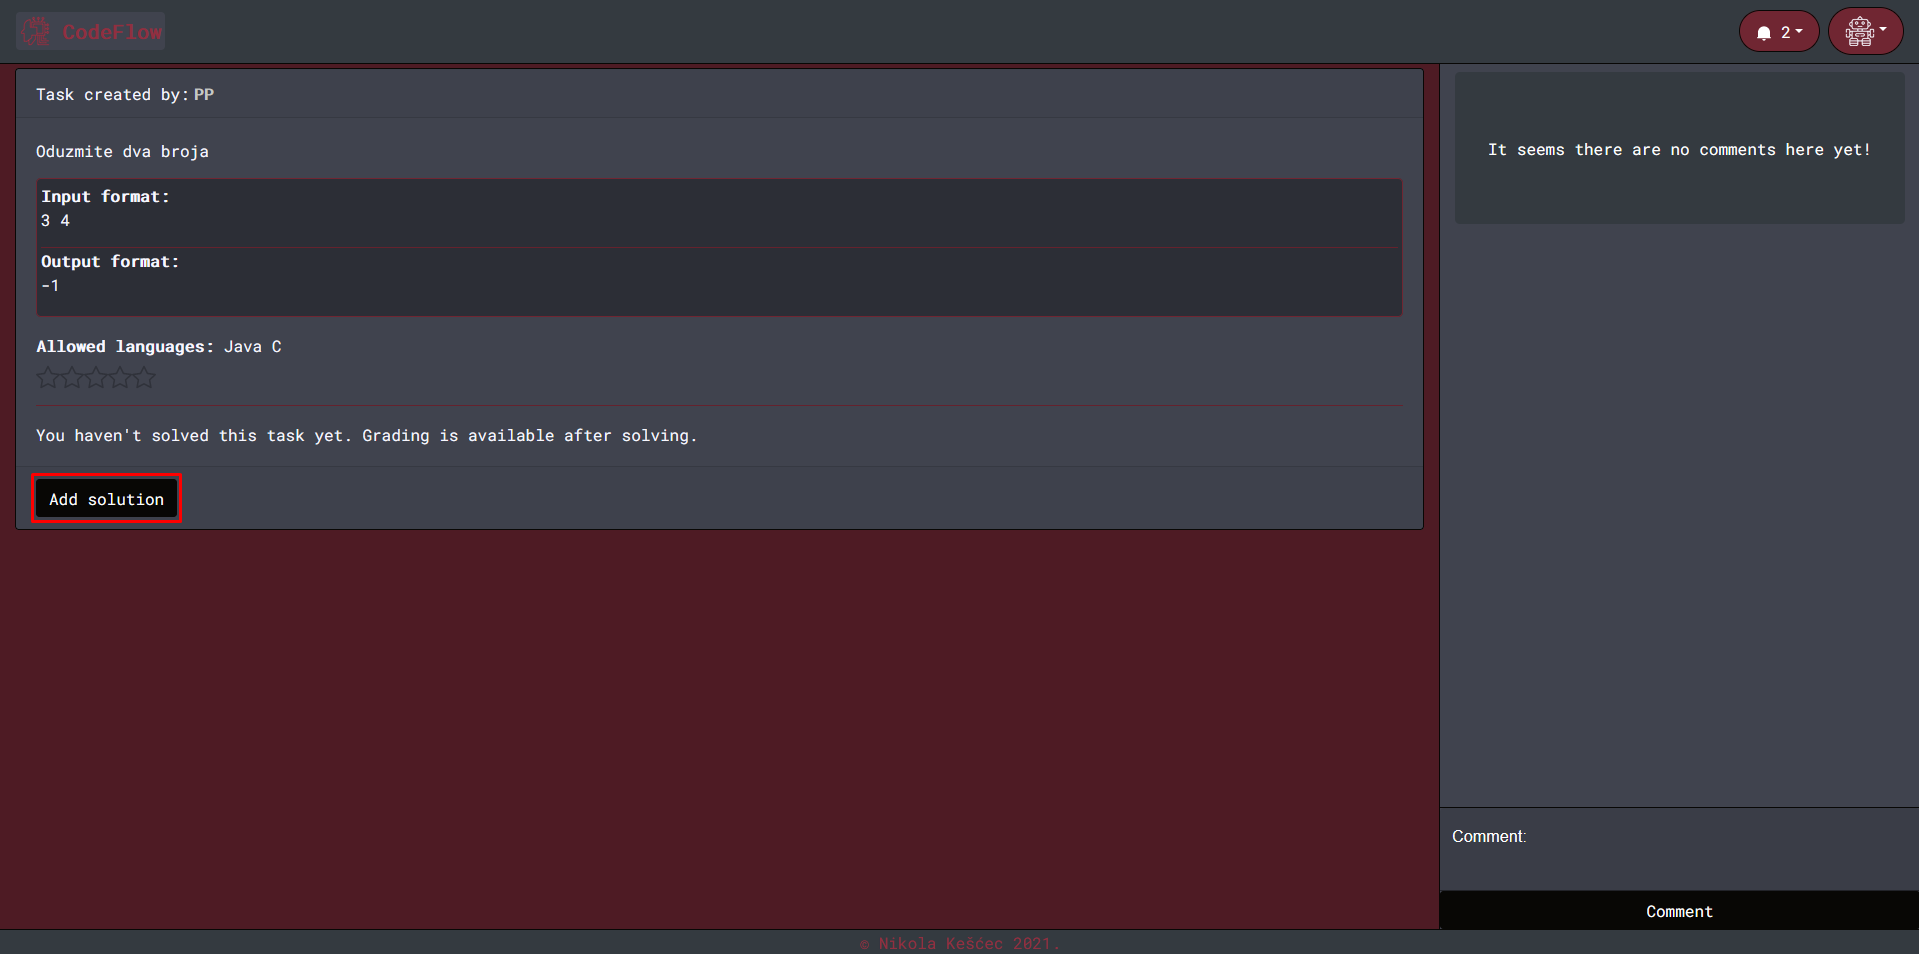
\includegraphics[width=\linewidth]{pictures/koristenje/DodajRjesenje.png}
			\caption{Prikaz detaljnog prikaza zadatka s naglašenim gumbom za dodavanje zadatka.}
			\label{fig:dodajrjesenje}
		\end{figure}
		\begin{figure}[H]
			\centering
			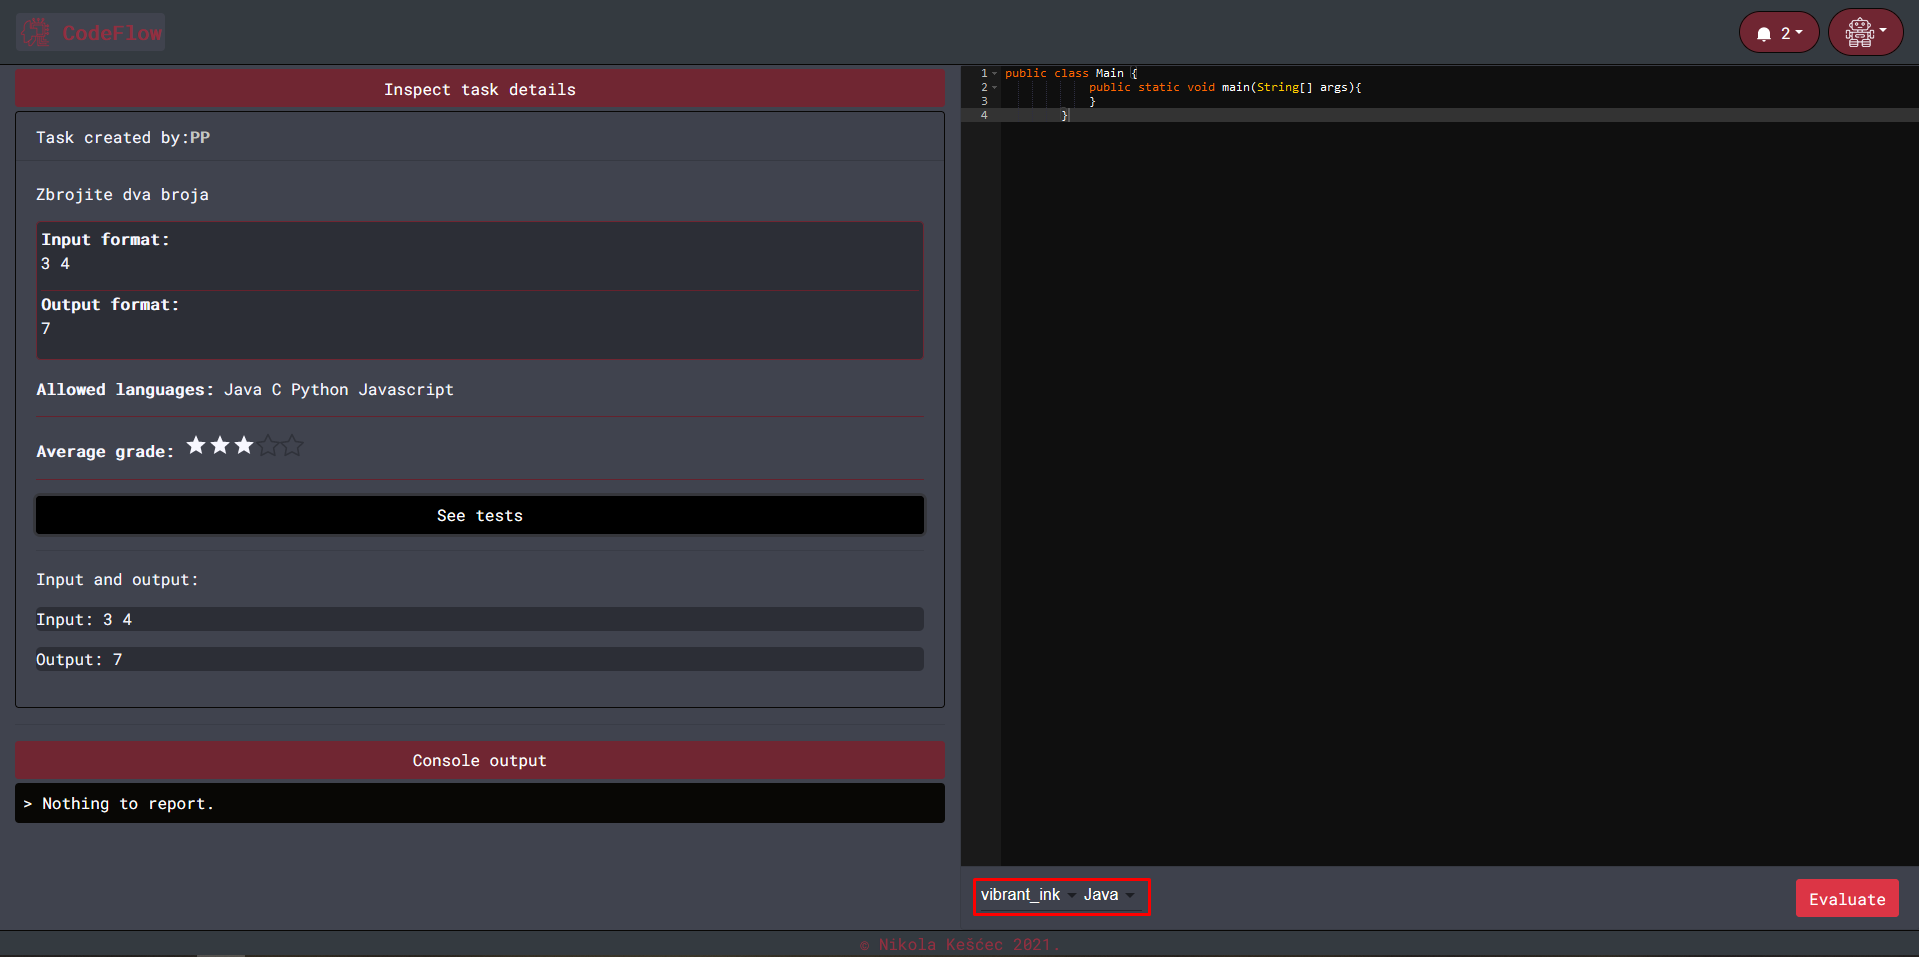
\includegraphics[width=\linewidth]{pictures/koristenje/StranicaRjesavanja.png}
			\caption{Prikaz stranice koja sadržava uređivač programskog koda s naglašenim opcijama za promjenu teme i programskog jezika.}
			\label{fig:rjesavanje}
		\end{figure}
		\begin{figure}[H]
			\centering
			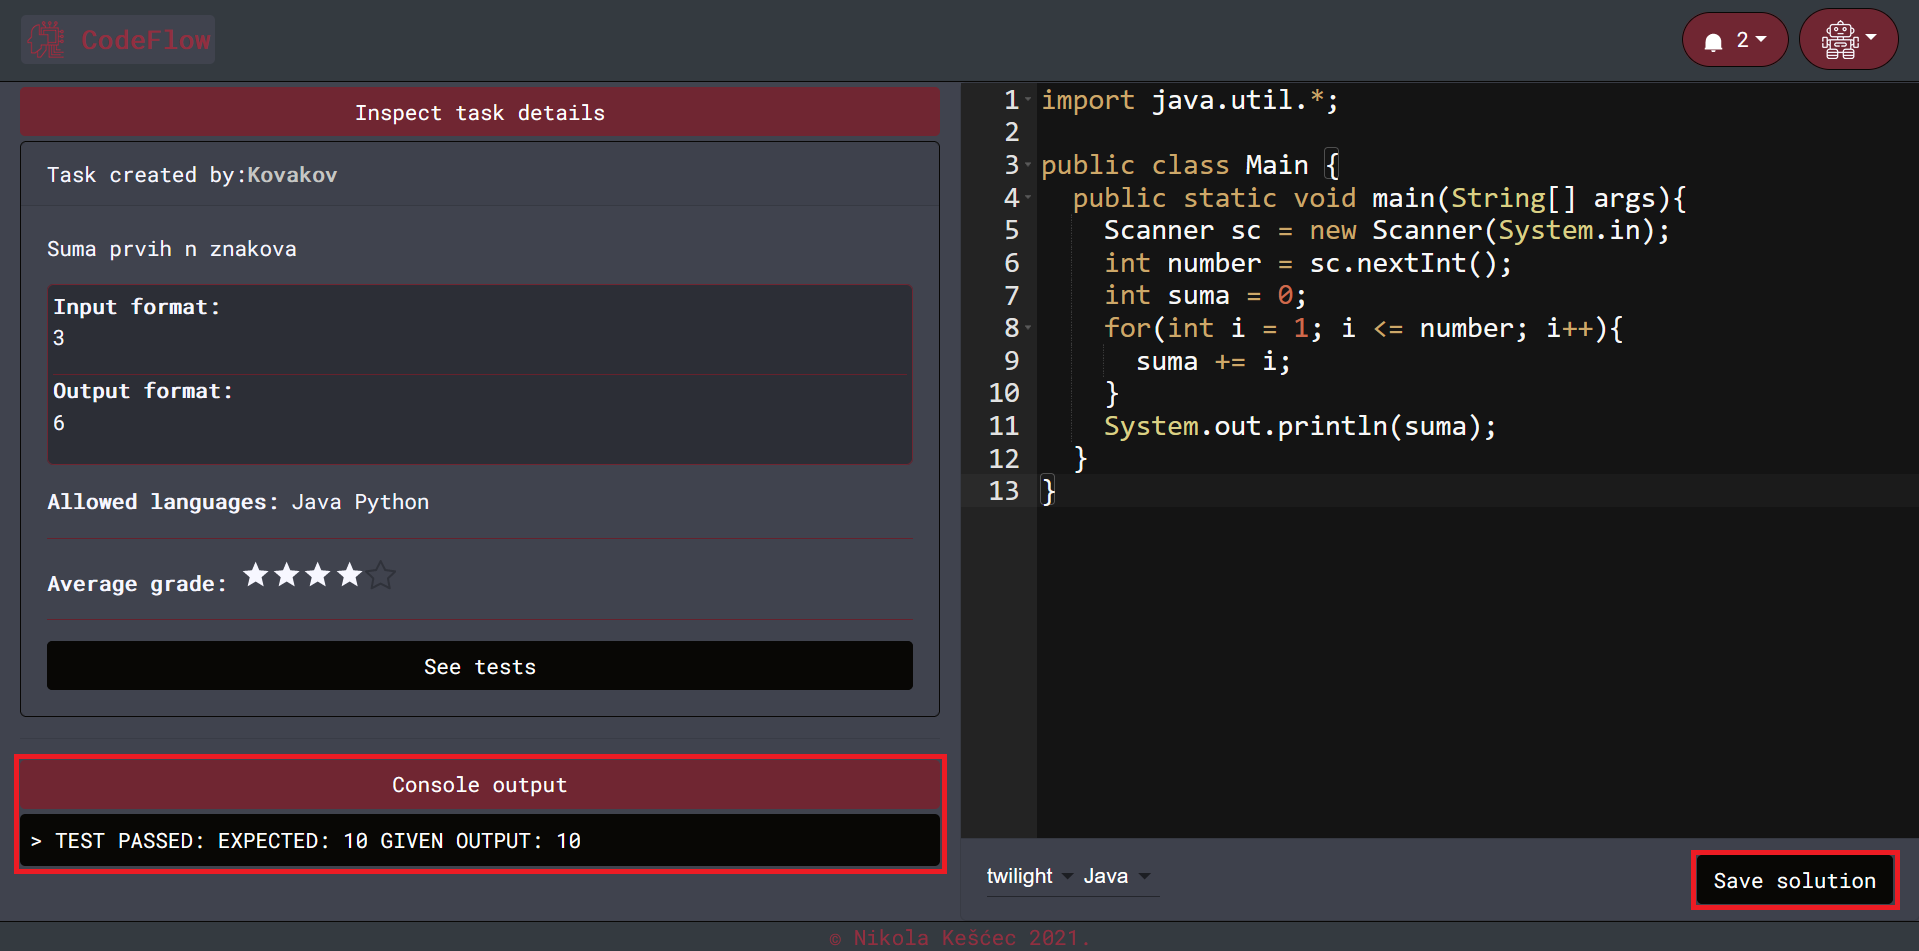
\includegraphics[width=\linewidth]{pictures/koristenje/RijeseniZadatak.png}
			\caption{Prikaz stranice koja sadržava uređivač programskog koda s evaluiranim rješenjem spremnim za pohranu. Naglašeni su rezultati evaluacije rješenja te gumb za spremanje rješenja.}
			\label{fig:rjeseno}
		\end{figure}
	
		\section{Stvaranje zadatka}
		Uz pregledavanje zadataka i rješenja te pisanja rješenja za odabrani zadatak, korisnici imaju pravo u bilo kojem trenutku napraviti zadatak. Poveznica koja vodi do stranice koja sadržava formu za stvaranje zadatka nalazi se unutar \textit{dropdown} gumba naglašenog na slici \ref{fig:dropdowntask}. Pritiskom na nju korisnici su odvedeni na stranicu na kojoj mogu definirati svoj zadatak. Stranica sadržava formu koja deklarira potrebne podatke za stvaranje programskog zadatka. Ti podaci redom su: opis zadatka, primjer ulaza i izlaza, dopušteni jezici te lista testnih slučajeva koji zadržavaju par ulaznih i izlaznih vrijednosti (redom numerirani na slici \ref{fig:stvaranjeforma}). Svaki od traženih podataka obavezan je te pojedinačno definiraju dodatne uvjete. Pojedinačni uvjeti su da opis zadatka ne smije biti kraći od 25 riječi, bar jedan programski jezik mora biti odabran te bar jedan testni zadatak mora biti definiran s popunjenim parom ulaznih i izlaznih vrijednosti. Tek nakon što korisnici zadovolje tražene uvjete mogu stvoriti novi zadatak.
		\begin{figure}[H]
			\centering
			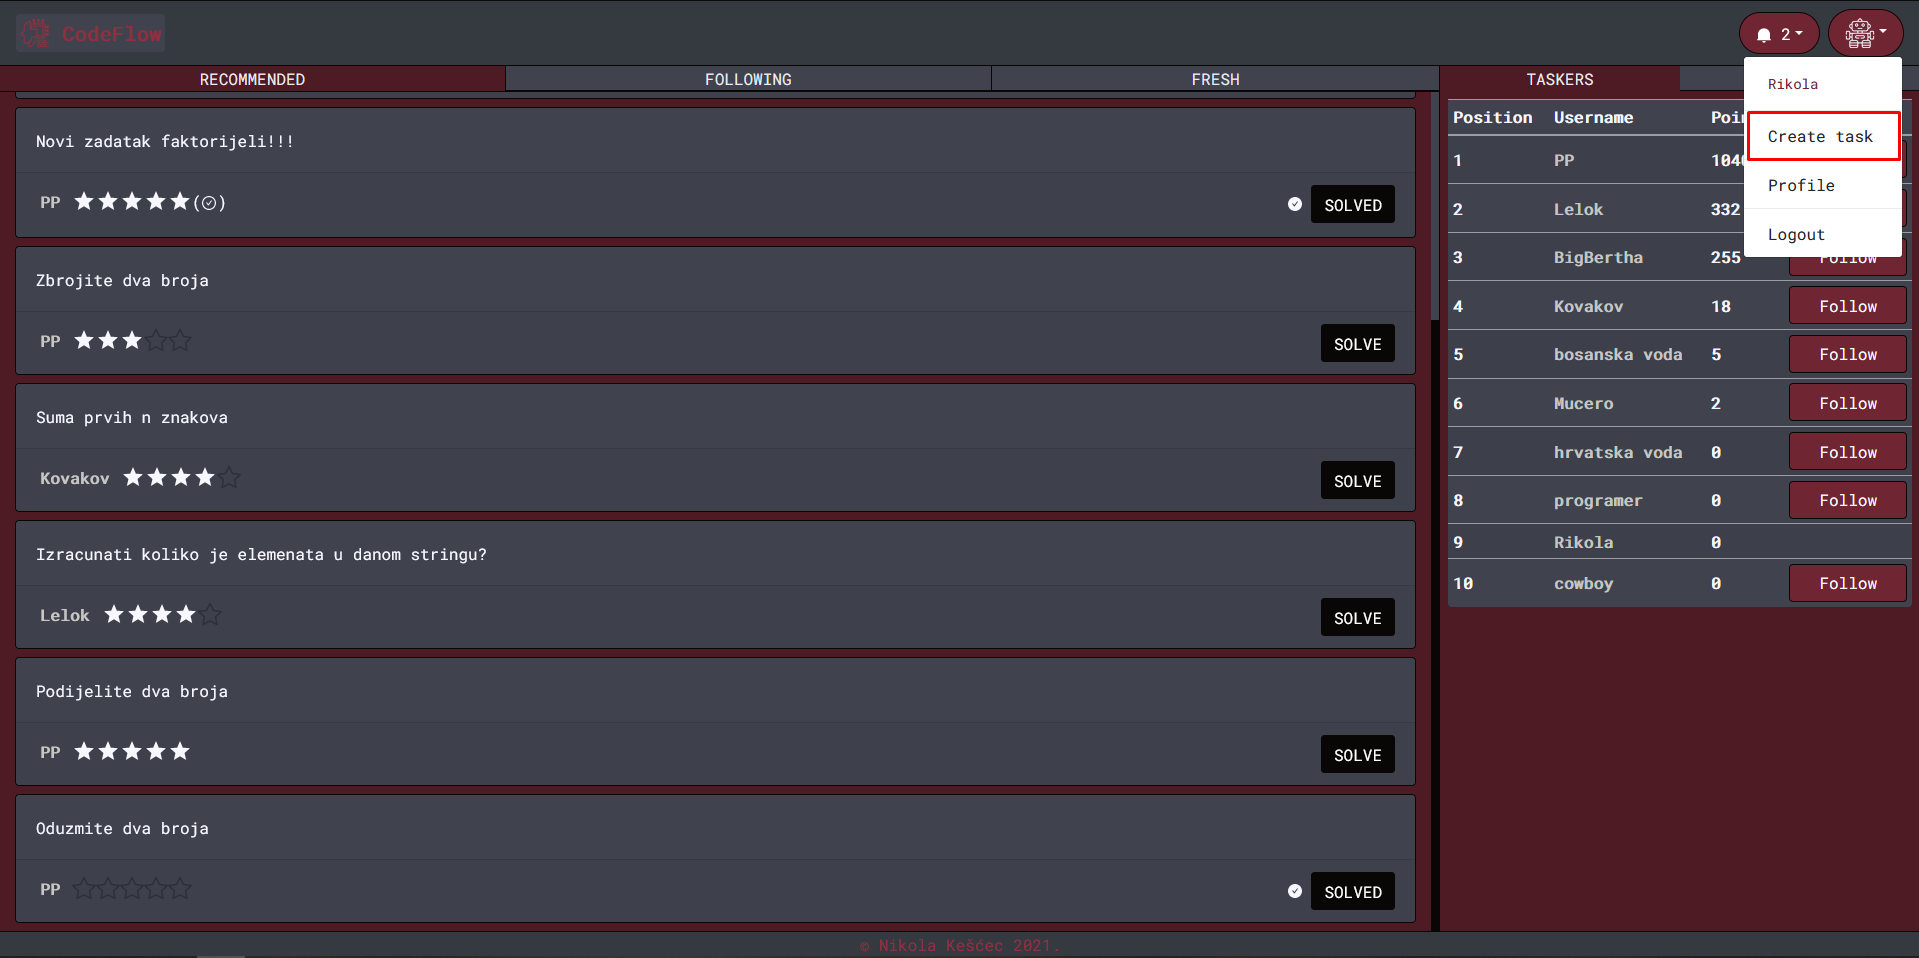
\includegraphics[scale=0.65]{pictures/koristenje/StvoriDropdown.png}
			\caption{Prikaz poveznice koja vodi na stranicu za stvaranje zadatka. Prikazivanje poveznice ostvaruje se pritiskom na označeni gumb.}
			\label{fig:dropdowntask}
		\end{figure}
		\begin{figure}[H]
			\centering
			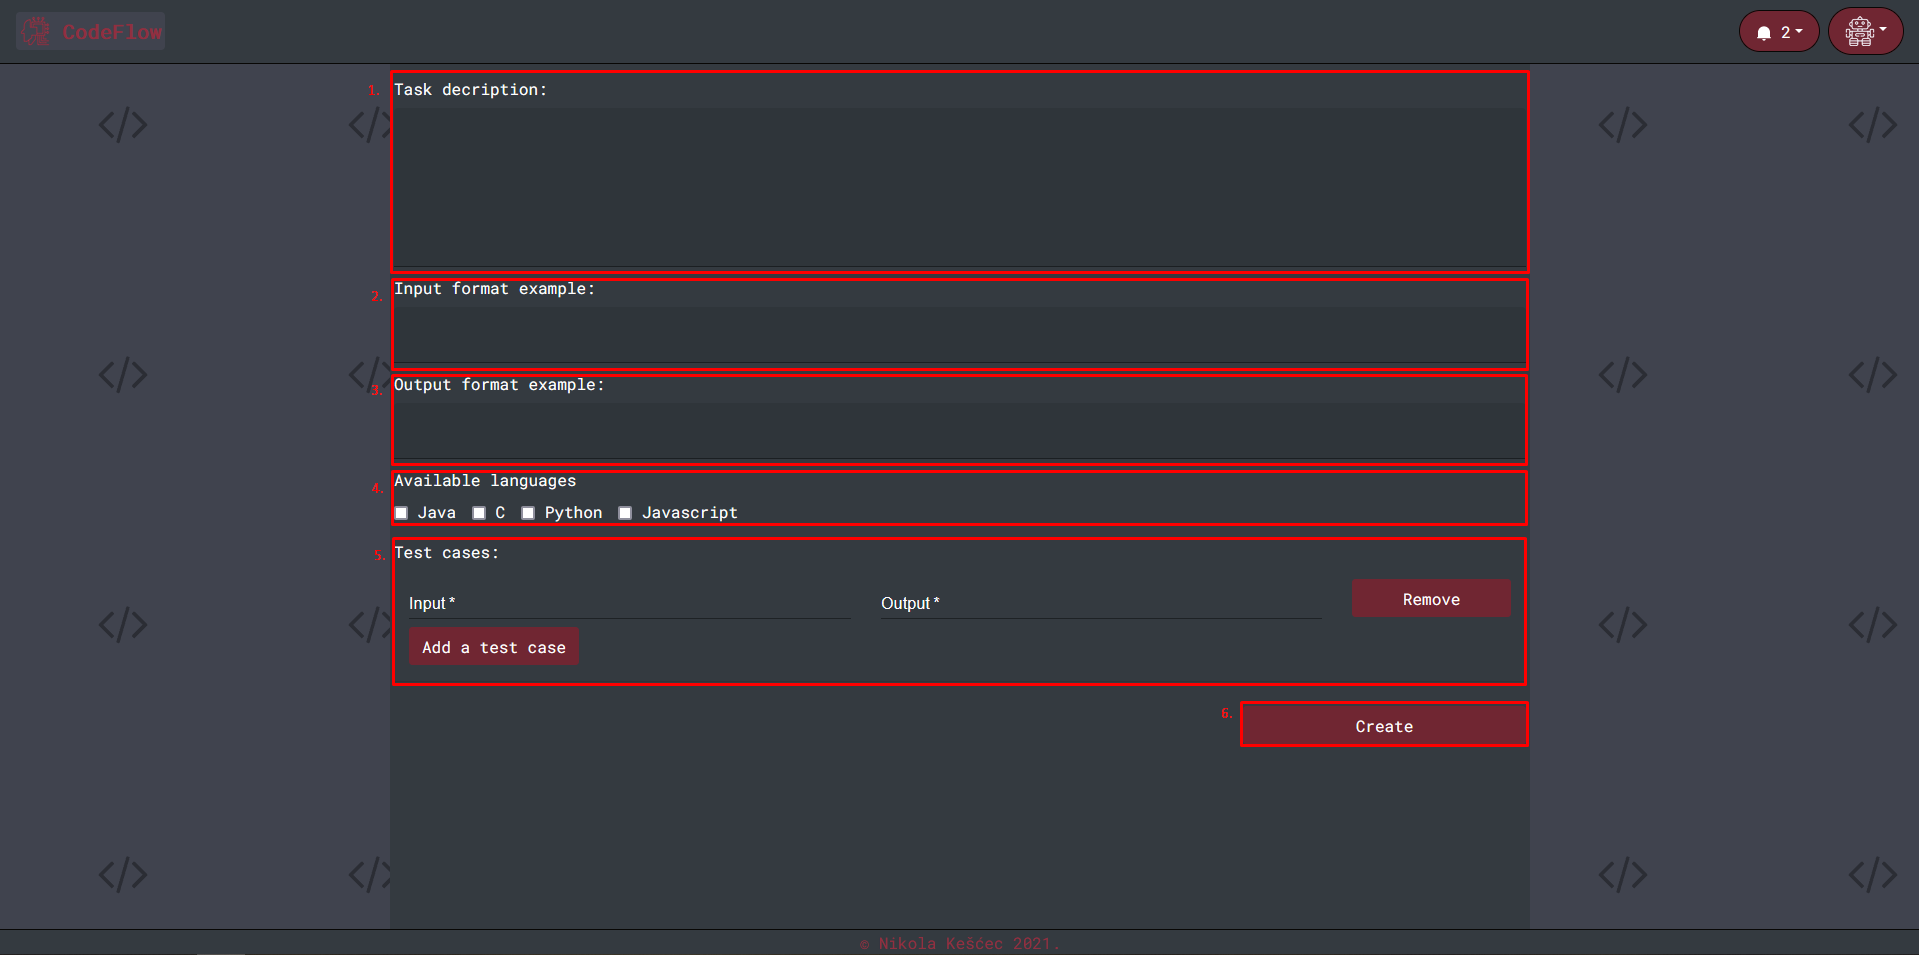
\includegraphics[width=\linewidth]{pictures/koristenje/FormaStvaranja.png}
			\caption{Prikaz forme za stvaranje zadatka s označenim traženim vrijednostima.}
			\label{fig:stvaranjeforma}
		\end{figure}
		
	\chapter{Budući razvoj}
	Codeflow aplikacija sadržava potencijal za dodavanje funkcionalnosti i unaprjeđenje postojećih. Dizajnirana je na način da dodavanje novih funkcionalnosti ne mijenja funkcionalnost već ostvarenih funkcionalnosti te je time otvorena za nadogradnju.
	Dakle, budući razvitak podijeljen je na kategoriju \textbf{nadogradnji} i \textbf{unaprjeđenja}.
	\subsubsection{Nadogradnje}
	Prva preporučena nadogradnja aplikacija bilo bi uvođenje sistema "igrifikacije" (spomenuto unutar potpoglavlja \ref{sec:codewars}). Uvođenje znački, kategorija i povremenih natjecanja pozitivno bi utjecalo na sveukupno korisničko iskustvo.\\
	Nedostatak trenutačnog sustava komentiranja i obavijesti u usporedbi s ostalim sličnim stranicama jest potreba za promjenom stranice ili, u najgorem slučaju, ponovnim učitavanjem aplikacije radi učitavanja promjena unutar komentara ili obavijesti. Ovaj nedostatak rješiv je korištenjem \textbf{WebSocket} protokola. WebSocket\cite{websocket2021} protokol omogućuje potpuno dvosmjernu komunikaciju između klijenta i poslužitelja u stvarnom vremenu. Makar različit od tipičnog HTTP protokola, dizajniran je da radi na istim vratima \engl{ports} (443 i 80) kao i HTTP protokol, što ga čini veoma prihvatljivim za normalnu internetsku interakciju između klijenta i poslužitelja. Podržan je na svim modernim internetskim preglednicima i njegovo bi svojstvo dvosmjerne komunikacije omogućilo internetskom pregledniku da ažuriranje komentara i obavijesti istovremeno dojavi i React aplikaciji na prezentacijskom sloju. React aplikacija bi potom ažurirala svoje korisničko sučelje da ispravno prati stanje podataka unutar podatkovnog sloja. Takav sistem bio bi prigodniji trenutačnom te bi kao nadogradnja potpuno zamijenio trenutačni.
	\subsubsection{Unaprjeđenja}
	Najvažnije unaprjeđenje bilo bi dodatna prilagodba sustava evaluacije korisničkih rješenja. Sustav u trenutnom stanju šalje rješenje pojedinačno za svaki testni slučaj tijekom evaluacije, što nije održivo za veća rješenja i veći broj testnih slučajeva. Unaprjeđenje bi sustav prilagodilo da umjesto pojedinačnog slanja pripremi takozvanu skupnu \engl{batched} pošiljku i obavi sve evaluacije u okviru jednog zahtjeva.\\
	Unaprjeđenje sustava spremanja rješenja koje bi bilo pogodno implementirati jest provjera plagijata tijekom dodavanja novog rješenja. Trenutačna verzija aplikacije ne provjerava sličnost rješenja te korisnici mogu veoma jednostavno u potpunosti kopirati već postojeća rješenja drugih korisnika. Sustav spremanja također ne pruža mogućnost spremanja nedovršenog rješenja programskog zadatka. Dodavanje te mogućnosti uveliko bi poboljšalo korisničko iskustvo te je još jedno od poželjnih unaprjeđenja.
	
	
	\chapter{Zaključak}
	Velik porast zanimanja za programiranjem te sve veća potreba za održavanjem programerskog znanja rezultirala je nastankom stranica koje omogućuju vježbanje i razvijanje programerskih vještina. Neke od stranica usvojile su elemente socijalnih mreža, poput dodavanja mogućnosti raspravljanja i komentiranja zadataka i rješenja, a sve češća je i implementacija sustava "igrifikacije". Doduše, učestali zajednički čimbenik navedenih stranica jest nemogućnost da prosječni korisnik zada zadatak. Ipak, zbog podržanih funkcionalnosti rješavanja zadataka, određenih socijalnih elemenata i implementacije navedenih sustava "igrifikacije" popularnost tih stranica visoka je.\\
	Tema ovog završnog rada bila je razvijanje i implementiranje aplikacije koja podržava učestale značajke popularnih stranica koje omogućavaju rješavanje programskih zadataka. Dodatne funkcionalnosti ove aplikacije su podržavanje najbitnijih elemenata socijalnih mreža i mogućnost zadavanja zadataka od strane bilo kojeg korisnika. \\
	Izazovan element izrade aplikacije koja zadovoljava spomenute zahtjeve bio je organizacija i strukturiranje sustava za stvaranje zadataka i pripremanje okvirnih predložaka za rješenja stvorenih zadataka. Jednako je izazovan element razvoja aplikacije ovoga specifičnoga tipa bio podržavanje provjeravanja ispravnosti korisničkog programskog koda. Ipak, uz pomoć Judge0 izvršitelja programskog koda i ta funkcionalnost uspješno je podržana.\\
	Odabir Spring radnog okvira i React JavaScript biblioteke bio je kvalitetan jer obje spomenute tehnologije posjeduju bogatu podršku te veoma kvalitetnu dokumentaciju. Također, spomenute tehnologije kvalitetno podržavaju izradu višeslojnih internetskih aplikacija te su uz kombinaciju PostgreSQL sustava za upravljanje bazama podataka potpuno zadovoljile tehnološke potrebe ovog završnog rada.\\
	
	
	

	\bibliography{literatura}
	\bibliographystyle{fer}
	
	\begin{sazetak}
		
		
		\kljucnerijeci{Spring, REST, React, SPA, JWT, PostgreSQL, zadavanje programskih zadataka.}
	\end{sazetak}
	
	% TODO: Navedite naslov na engleskom jeziku.
	\engtitle{Web application for solving programming tasks with social network elements}
	\begin{abstract}
		
		
		\keywords{Spring, REST, React, SPA, JWT, PostgreSQL, programing problems assingment.}
	\end{abstract}
	
\end{document}
